% Capitolul 14: Inferență cauzală pentru serii de timp
% Analiza avansată a seriilor de timp și previziune -- Programul de master Statistică aplicată și data science, anul I, semestrul 2, Academia de Studii Economice din București
% GENERAT de latex/build_chapter14.py -- modificați generatorul, nu acest fișier.

\newcommand{\coursename}{Analiza avansată a seriilor de timp și previziune}
\def\atslang{ro}
% Preambul comun ATS -- Analiza avansată a seriilor de timp și previziune / Advanced Time Series Analysis and Forecasting
% (Beamer, 16:9). Același design ca MFM, SFM și TSA (copiat din TSA, 5 octombrie 2026). Înainte de % Preambul comun ATS -- Analiza avansată a seriilor de timp și previziune / Advanced Time Series Analysis and Forecasting
% (Beamer, 16:9). Același design ca MFM, SFM și TSA (copiat din TSA, 5 octombrie 2026). Înainte de % Preambul comun ATS -- Analiza avansată a seriilor de timp și previziune / Advanced Time Series Analysis and Forecasting
% (Beamer, 16:9). Același design ca MFM, SFM și TSA (copiat din TSA, 5 octombrie 2026). Înainte de \input{../../latex/preamble} se definește
%   \newcommand{\coursename}{Advanced Time Series Analysis and Forecasting}          (EN)
%   \newcommand{\coursename}{Analiza avansată a seriilor de timp și previziune}       (RO)  și  \def\atslang{ro}
% Fișierele .tex se află în EN/Courses, EN/Seminars, RO/Cursuri, RO/Seminarii (două niveluri sub rădăcină).
% Deck-urile sînt generate de latex/build_chapterN.py / build_seminarN.py (vezi latex/ats_build.py).

\documentclass[9pt, aspectratio=169, t]{beamer}
\providecommand{\coursename}{Advanced Time Series Analysis and Forecasting}

% Ensure content fits on slides
\setbeamersize{text margin left=8mm, text margin right=8mm}
% Smaller institute font (title page)
\setbeamerfont{institute}{size=\footnotesize}

%=============================================================================
% THEME AND STYLE CONFIGURATION
%=============================================================================
\usetheme{default}
% Using default theme for clean header/footer control

% Color Palette (matching Redispatch PDF)
\definecolor{MainBlue}{RGB}{26, 58, 110}
\definecolor{AccentBlue}{RGB}{26, 58, 110}
\definecolor{IDAred}{RGB}{205, 0, 0}
\definecolor{DarkGray}{RGB}{51, 51, 51}
\definecolor{MediumGray}{RGB}{128, 128, 128}
\definecolor{LightGray}{RGB}{248, 248, 248}
\definecolor{VeryLightGray}{RGB}{235, 235, 235}
\definecolor{KeynoteGray}{RGB}{218, 218, 218}
\definecolor{SectionGray}{RGB}{120, 120, 120}
\definecolor{FooterGray}{RGB}{100, 100, 100}
\definecolor{Crimson}{RGB}{220, 53, 69}
\definecolor{Forest}{RGB}{46, 125, 50}
\definecolor{Amber}{RGB}{181, 133, 63}
\definecolor{Orange}{RGB}{230, 126, 34}
\definecolor{Purple}{RGB}{142, 68, 173}

% Gradient background (exact Keynote 315° gradient: white to RGB 218,218,218)
\setbeamertemplate{background}{%
    \begin{tikzpicture}[remember picture, overlay]
        \shade[shading=axis, shading angle=315,
        top color=white, bottom color=KeynoteGray]
        (current page.south west) rectangle (current page.north east);
    \end{tikzpicture}%
}
% Fallback solid color for compatibility
\setbeamercolor{background canvas}{bg=}

\setbeamercolor{palette primary}{bg=MainBlue, fg=white}
\setbeamercolor{palette secondary}{bg=MainBlue!85, fg=white}
\setbeamercolor{palette tertiary}{bg=MainBlue!70, fg=white}
\setbeamercolor{structure}{fg=MainBlue}
\setbeamercolor{title}{fg=IDAred}
\setbeamercolor{frametitle}{fg=IDAred, bg=}
\setbeamercolor{block title}{bg=MainBlue, fg=white}
\setbeamercolor{block body}{bg=VeryLightGray, fg=DarkGray}
\setbeamercolor{block title alerted}{bg=Crimson, fg=white}
\setbeamercolor{block body alerted}{bg=Crimson!8, fg=DarkGray}
\setbeamercolor{block title example}{bg=Forest, fg=white}
\setbeamercolor{block body example}{bg=Forest!8, fg=DarkGray}
\setbeamercolor{item}{fg=MainBlue}

% Footer colors (override Madrid theme blue)
\setbeamercolor{author in head/foot}{fg=FooterGray, bg=}
\setbeamercolor{title in head/foot}{fg=FooterGray, bg=}
\setbeamercolor{date in head/foot}{fg=FooterGray, bg=}
\setbeamercolor{section in head/foot}{fg=FooterGray, bg=}
\setbeamercolor{subsection in head/foot}{fg=FooterGray, bg=}

% Bullet styles (apply everywhere including blocks)
\setbeamertemplate{itemize item}{\color{MainBlue}$\boxdot$}
\setbeamertemplate{itemize subitem}{\color{MainBlue}$\blacktriangleright$}
\setbeamertemplate{itemize subsubitem}{\color{MainBlue}\tiny$\bullet$}
\setbeamertemplate{itemize/enumerate body begin}{\normalsize}
\setbeamertemplate{itemize/enumerate subbody begin}{\normalsize}

% Item spacing - compact style
\setlength{\leftmargini}{10pt}       % Level 1: minimal indent
\setlength{\leftmarginii}{10pt}      % Level 2: minimal additional indent
% Compact list spacing (zero extra space before/after lists in blocks)
\makeatletter
\def\@listi{\leftmargin\leftmargini \topsep 0pt \parsep 0pt \itemsep 0pt}
\def\@listii{\leftmargin\leftmarginii \topsep 0pt \parsep 0pt \itemsep 0pt}
\makeatother

\setbeamertemplate{navigation symbols}{}

%=============================================================================
% CUSTOM HEADLINE
%=============================================================================
\setbeamertemplate{headline}{%
    \vskip10pt%
    \hbox to \paperwidth{%
        \hskip0.5cm%
        {\small\color{FooterGray}\renewcommand{\hyperlink}[2]{##2}\insertsectionhead}%
        \hfill%
        \textcolor{FooterGray}{\small\insertframenumber}%
        \hskip0.5cm%
    }%
    \vskip4pt%
    {\color{FooterGray}\hrule height 0.4pt}%
}

%=============================================================================
% CUSTOM FOOTER
%=============================================================================
\usepackage{fontawesome5}

\setbeamertemplate{footline}{%
    {\color{FooterGray}\hrule height 0.4pt}%
    \vskip4pt%
    \hbox to \paperwidth{%
        \hskip0.5cm%
        \textcolor{FooterGray}{\small\coursename}%
        \hfill%
        \raisebox{-0.1em}{%
            \begin{tikzpicture}[x=0.08em, y=0.08em, line width=0.4pt]
                \draw[FooterGray] (0,3) -- (1,4) -- (2,3.5) -- (3,5) -- (4,4) -- (5,6) -- (6,5.5) -- (7,4) -- (8,5) -- (9,7) -- (10,6) -- (11,5) -- (12,6.5) -- (13,8) -- (14,7) -- (15,6) -- (16,7.5) -- (17,9) -- (18,8) -- (19,7) -- (20,8.5) -- (21,10) -- (22,9) -- (23,8) -- (24,9.5);
            \end{tikzpicture}%
        }%
        \hskip0.5cm%
    }%
    \vskip6pt%
}

%=============================================================================
% PACKAGES
%=============================================================================
\usepackage[utf8]{inputenc}
\DeclareUnicodeCharacter{03B1}{\ensuremath{\alpha}}
\usepackage[T1]{fontenc}
\usepackage{amsmath, amssymb, amsthm}
\usepackage{mathtools}
\usepackage{bm}
\usepackage{tikz}
\usetikzlibrary{arrows.meta, positioning, shapes, calc, decorations.pathreplacing, shadings}
\usepackage{booktabs}
\usepackage{multirow}
\usepackage{array}
\usepackage{graphicx}
\usepackage{animate}
\usepackage{hyperref}
\usepackage{colortbl}
\usepackage{listings}
\lstset{language=Python, basicstyle=\ttfamily\scriptsize, keywordstyle=\color{MainBlue}\bfseries,
  commentstyle=\color{Forest}, stringstyle=\color{Crimson}, breaklines=true,
  frame=none, backgroundcolor=\color{VeryLightGray}, xleftmargin=2mm}
\hypersetup{colorlinks=true, linkcolor=MainBlue, urlcolor=MainBlue}
\graphicspath{{../../logos/}{../../charts/}{../../photos/}}
\usepackage{xcolor}
\hfuzz=2pt  % Suppress tiny overfull warnings (<2pt)
\vfuzz=2pt  % Suppress tiny vertical overfull warnings (<2pt)

%=============================================================================
% QUANTLET COMMANDS
%   \quantlet{<displayed name>}{<url>}       (generic)
%   \atsquantlet{Ch_05}{ATS_ch5_garch}       -> https://github.com/danpele/Advanced-Time-Series/tree/main/Quantlets/Ch_05/ATS_ch5_garch
%   \qlurl{<folder>} is defined per chapter by the generator (Quantlets/Ch_NN/<folder>)
%=============================================================================
\newcommand{\atsrepo}{https://github.com/danpele/Advanced-Time-Series}
\newcommand{\atsqlbase}{https://github.com/danpele/Advanced-Time-Series/tree/main/Quantlets}
\newcommand{\quantlet}[2]{%
    \hfill\href{#2}{%
        \raisebox{-0.15em}{
\includegraphics[height=0.7em]{ql_logo.png}}%
        \textcolor{MainBlue}{\tiny\ #1}%
    }%
}
\newcommand{\atsquantlet}[2]{\quantlet{\detokenize{#2}}{\atsqlbase/#1/#2}}

%=============================================================================
% NOTEBOOKS (Google Colab)
%   \colaburl{notebooks/EN/chapter5_seminar_notebook.ipynb} -> the Colab link of a file in the ATS repo
%   \nb: the chapter notebook (each seminar deck redefines it with \renewcommand)
%=============================================================================
\newcommand{\colaburl}[1]{https://colab.research.google.com/github/danpele/Advanced-Time-Series/blob/main/#1}
\newcommand{\nb}{https://colab.research.google.com/github/danpele/Advanced-Time-Series/tree/main/notebooks/EN}
\newcommand{\nbname}{notebooks/EN}

%=============================================================================
% SLIDE HELPERS (used by the generators; the same as in MFM)
%=============================================================================
% local font size for list bodies (the preamble forces \normalsize)
\newcommand{\itemsize}[1]{\setbeamertemplate{itemize/enumerate body begin}{#1}\setbeamertemplate{itemize/enumerate subbody begin}{#1}}
\newcommand{\intitle}[1]{{\hypersetup{urlcolor=white}#1}}   % white links inside coloured title bars
\newcommand{\imgcap}[1]{{\scriptsize #1}\\[0.5mm]}          % caption under a photo
\newcommand{\imgcredit}[2]{{\tiny\color{FooterGray}\href{#1}{#2}}}   % image credit: source URL, author/licence
\newcommand{\aiprompt}[1]{{\ttfamily\color{MainBlue}#1}}     % a prompt to an AI assistant

%=============================================================================
% SEMINARS: student version by default; the instructor wrapper *_solutions.tex sets \solutionstrue
%=============================================================================
\makeatletter\@ifundefined{ifsolutions}{\expandafter\newif\csname ifsolutions\endcsname}{}\makeatother
\newcommand{\solonly}[1]{\ifsolutions #1\fi}
\newcommand{\propsub}{\ifsolutions\else\framesubtitle{\ifdefined\atslang Rezolvarea se discută la seminar\else Solution discussed in class\fi}\fi}

%=============================================================================
% APPENDIX AND CHAPTER LINKS (latex/appendix_links.py writes the calls; it also re-declares these
% macros before \begin{document}, so the decks compile with or without this preamble block)
%=============================================================================
\providecommand{\atsapplink}[3]{\hypertarget{#2}{}\hyperlink{#1}{\beamergotobutton{#3}}}
\providecommand{\atsappback}[2]{\begin{tikzpicture}[remember picture,overlay]\node[anchor=south east] at ([xshift=-3mm,yshift=7mm]current page.south east){\hyperlink{#1}{\beamerreturnbutton{#2}}};\end{tikzpicture}}
\providecommand{\atschlink}[2]{\href{#1}{#2}}
\providecommand{\atschlinkt}[2]{\href{#1}{\usebeamercolor[fg]{frametitle}#2}}

%=============================================================================
% QUANTINAR COMMAND: link către un curs Quantinar (subiecte avansate)
%=============================================================================
\newcommand{\quantinar}[2]{%
    \href{#2}{%
        \raisebox{-0.15em}{
\includegraphics[height=0.8em]{qr_logo.png}}%
        \textcolor{MainBlue}{\scriptsize\ #1}%
    }%
}

%=============================================================================
% CUSTOM TITLE PAGE
%=============================================================================
\defbeamertemplate*{title page}{hybrid}[1][]
{
    \vspace{0.2cm}
    % Logos row - top header (with clickable links)
    \begin{center}
        \href{https://www.ase.ro}{
\includegraphics[height=1.0cm]{ase_logo.png}}\hspace{0.3cm}%
        \href{https://theida.net}{
\includegraphics[height=1.0cm]{ida_logo.png}}\hspace{0.3cm}%
        \href{https://blockchain-research-center.com}{
\includegraphics[height=1.0cm]{brc_logo.png}}\hspace{0.3cm}%
        \href{https://www.ai4efin.ase.ro}{
\includegraphics[height=1.0cm]{ai4efin_logo.png}}\hspace{0.3cm}%
        \href{https://ipe.ro/new}{
\includegraphics[height=1.0cm]{acad_logo.png}}\hspace{0.3cm}%
        \href{https://www.digital-finance-msca.com}{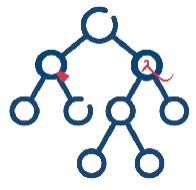
\includegraphics[height=1.0cm]{msca_logo.png}}%
    \end{center}

    \vspace{0.6cm}

    % Main title with Q logos on sides (with clickable links)
    \begin{center}
        \begin{minipage}{0.1\textwidth}
            \centering
            \href{https://quantlet.com}{
\includegraphics[height=1.1cm]{ql_logo.png}}
        \end{minipage}%
        \begin{minipage}{0.78\textwidth}
            \centering
            {\LARGE\bfseries\usebeamercolor[fg]{title}\inserttitle}

            \vspace{0.3cm}

            {\usebeamerfont{subtitle}\usebeamercolor[fg]{title}\insertsubtitle}
        \end{minipage}%
        \begin{minipage}{0.1\textwidth}
            \centering
            \href{https://quantinar.com}{
\includegraphics[height=1.1cm]{qr_logo.png}}
        \end{minipage}
    \end{center}

    \vspace{0.6cm}

    % Authors (left aligned)
    \hspace{0.5cm}{\usebeamerfont{author}\insertauthor}

    \vspace{0.3cm}

    % Institute/Affiliations (left aligned)
    \hspace{0.5cm}\begin{minipage}[t]{0.9\textwidth}
        \raggedright\small\insertinstitute
    \end{minipage}
}

%=============================================================================
% THEOREM ENVIRONMENTS
%=============================================================================
\theoremstyle{definition}
\setbeamertemplate{theorems}[numbered]
\ifdefined\atslang
\newtheorem{defn}{Definiție}
\newtheorem{thm}{Teoremă}
\newtheorem{prop}{Propoziție}
\newtheorem{rmk}{Observație}
\else
\newtheorem{defn}{Definition}
\newtheorem{thm}{Theorem}
\newtheorem{prop}{Proposition}
\newtheorem{rmk}{Remark}
\fi

%=============================================================================
% CENTRED MINIPAGE (no extra vertical space)
%=============================================================================
\newenvironment{cminipage}[1]{%
    \par\noindent\hfill\begin{minipage}{#1}\ignorespaces
}{%
    \end{minipage}\hfill\null\par
}

%=============================================================================
% CUSTOM COMMANDS
%=============================================================================
\newcommand{\E}{\mathbb{E}}
\newcommand{\Var}{\text{Var}}
\newcommand{\Cov}{\text{Cov}}
\newcommand{\Corr}{\text{Corr}}
\newcommand{\R}{\mathbb{R}}
\newcommand{\N}{\mathbb{N}}
\newcommand{\Z}{\mathbb{Z}}
\newcommand{\B}{\mathbf{B}}
\newcommand{\imark}{\textcolor{MainBlue}{\textbullet}}
\newcommand{\RMSE}{\text{RMSE}}
\newcommand{\MAE}{\text{MAE}}
\newcommand{\MAPE}{\text{MAPE}}

% Boldface vector/matrix commands (VAR, VECM, state space)
\newcommand{\bY}{\mathbf{Y}}
\newcommand{\bX}{\mathbf{X}}
\newcommand{\bA}{\mathbf{A}}
\newcommand{\bB}{\mathbf{B}}
\newcommand{\bepsilon}{\boldsymbol{\varepsilon}}
\newcommand{\bSigma}{\boldsymbol{\Sigma}}
\newcommand{\bPhi}{\boldsymbol{\Phi}}
\newcommand{\bGamma}{\boldsymbol{\Gamma}}
\newcommand{\bPi}{\boldsymbol{\Pi}}
\newcommand{\bc}{\mathbf{c}}
\newcommand{\balpha}{\boldsymbol{\alpha}}
\newcommand{\bbeta}{\boldsymbol{\beta}}
\newcommand{\bvarepsilon}{\boldsymbol{\varepsilon}}

% Seminar marks
\newcommand{\correct}{\textcolor{Forest}{\checkmark}}
\newcommand{\incorrect}{\textcolor{Crimson}{\texttimes}}
 se definește
%   \newcommand{\coursename}{Advanced Time Series Analysis and Forecasting}          (EN)
%   \newcommand{\coursename}{Analiza avansată a seriilor de timp și previziune}       (RO)  și  \def\atslang{ro}
% Fișierele .tex se află în EN/Courses, EN/Seminars, RO/Cursuri, RO/Seminarii (două niveluri sub rădăcină).
% Deck-urile sînt generate de latex/build_chapterN.py / build_seminarN.py (vezi latex/ats_build.py).

\documentclass[9pt, aspectratio=169, t]{beamer}
\providecommand{\coursename}{Advanced Time Series Analysis and Forecasting}

% Ensure content fits on slides
\setbeamersize{text margin left=8mm, text margin right=8mm}
% Smaller institute font (title page)
\setbeamerfont{institute}{size=\footnotesize}

%=============================================================================
% THEME AND STYLE CONFIGURATION
%=============================================================================
\usetheme{default}
% Using default theme for clean header/footer control

% Color Palette (matching Redispatch PDF)
\definecolor{MainBlue}{RGB}{26, 58, 110}
\definecolor{AccentBlue}{RGB}{26, 58, 110}
\definecolor{IDAred}{RGB}{205, 0, 0}
\definecolor{DarkGray}{RGB}{51, 51, 51}
\definecolor{MediumGray}{RGB}{128, 128, 128}
\definecolor{LightGray}{RGB}{248, 248, 248}
\definecolor{VeryLightGray}{RGB}{235, 235, 235}
\definecolor{KeynoteGray}{RGB}{218, 218, 218}
\definecolor{SectionGray}{RGB}{120, 120, 120}
\definecolor{FooterGray}{RGB}{100, 100, 100}
\definecolor{Crimson}{RGB}{220, 53, 69}
\definecolor{Forest}{RGB}{46, 125, 50}
\definecolor{Amber}{RGB}{181, 133, 63}
\definecolor{Orange}{RGB}{230, 126, 34}
\definecolor{Purple}{RGB}{142, 68, 173}

% Gradient background (exact Keynote 315° gradient: white to RGB 218,218,218)
\setbeamertemplate{background}{%
    \begin{tikzpicture}[remember picture, overlay]
        \shade[shading=axis, shading angle=315,
        top color=white, bottom color=KeynoteGray]
        (current page.south west) rectangle (current page.north east);
    \end{tikzpicture}%
}
% Fallback solid color for compatibility
\setbeamercolor{background canvas}{bg=}

\setbeamercolor{palette primary}{bg=MainBlue, fg=white}
\setbeamercolor{palette secondary}{bg=MainBlue!85, fg=white}
\setbeamercolor{palette tertiary}{bg=MainBlue!70, fg=white}
\setbeamercolor{structure}{fg=MainBlue}
\setbeamercolor{title}{fg=IDAred}
\setbeamercolor{frametitle}{fg=IDAred, bg=}
\setbeamercolor{block title}{bg=MainBlue, fg=white}
\setbeamercolor{block body}{bg=VeryLightGray, fg=DarkGray}
\setbeamercolor{block title alerted}{bg=Crimson, fg=white}
\setbeamercolor{block body alerted}{bg=Crimson!8, fg=DarkGray}
\setbeamercolor{block title example}{bg=Forest, fg=white}
\setbeamercolor{block body example}{bg=Forest!8, fg=DarkGray}
\setbeamercolor{item}{fg=MainBlue}

% Footer colors (override Madrid theme blue)
\setbeamercolor{author in head/foot}{fg=FooterGray, bg=}
\setbeamercolor{title in head/foot}{fg=FooterGray, bg=}
\setbeamercolor{date in head/foot}{fg=FooterGray, bg=}
\setbeamercolor{section in head/foot}{fg=FooterGray, bg=}
\setbeamercolor{subsection in head/foot}{fg=FooterGray, bg=}

% Bullet styles (apply everywhere including blocks)
\setbeamertemplate{itemize item}{\color{MainBlue}$\boxdot$}
\setbeamertemplate{itemize subitem}{\color{MainBlue}$\blacktriangleright$}
\setbeamertemplate{itemize subsubitem}{\color{MainBlue}\tiny$\bullet$}
\setbeamertemplate{itemize/enumerate body begin}{\normalsize}
\setbeamertemplate{itemize/enumerate subbody begin}{\normalsize}

% Item spacing - compact style
\setlength{\leftmargini}{10pt}       % Level 1: minimal indent
\setlength{\leftmarginii}{10pt}      % Level 2: minimal additional indent
% Compact list spacing (zero extra space before/after lists in blocks)
\makeatletter
\def\@listi{\leftmargin\leftmargini \topsep 0pt \parsep 0pt \itemsep 0pt}
\def\@listii{\leftmargin\leftmarginii \topsep 0pt \parsep 0pt \itemsep 0pt}
\makeatother

\setbeamertemplate{navigation symbols}{}

%=============================================================================
% CUSTOM HEADLINE
%=============================================================================
\setbeamertemplate{headline}{%
    \vskip10pt%
    \hbox to \paperwidth{%
        \hskip0.5cm%
        {\small\color{FooterGray}\renewcommand{\hyperlink}[2]{##2}\insertsectionhead}%
        \hfill%
        \textcolor{FooterGray}{\small\insertframenumber}%
        \hskip0.5cm%
    }%
    \vskip4pt%
    {\color{FooterGray}\hrule height 0.4pt}%
}

%=============================================================================
% CUSTOM FOOTER
%=============================================================================
\usepackage{fontawesome5}

\setbeamertemplate{footline}{%
    {\color{FooterGray}\hrule height 0.4pt}%
    \vskip4pt%
    \hbox to \paperwidth{%
        \hskip0.5cm%
        \textcolor{FooterGray}{\small\coursename}%
        \hfill%
        \raisebox{-0.1em}{%
            \begin{tikzpicture}[x=0.08em, y=0.08em, line width=0.4pt]
                \draw[FooterGray] (0,3) -- (1,4) -- (2,3.5) -- (3,5) -- (4,4) -- (5,6) -- (6,5.5) -- (7,4) -- (8,5) -- (9,7) -- (10,6) -- (11,5) -- (12,6.5) -- (13,8) -- (14,7) -- (15,6) -- (16,7.5) -- (17,9) -- (18,8) -- (19,7) -- (20,8.5) -- (21,10) -- (22,9) -- (23,8) -- (24,9.5);
            \end{tikzpicture}%
        }%
        \hskip0.5cm%
    }%
    \vskip6pt%
}

%=============================================================================
% PACKAGES
%=============================================================================
\usepackage[utf8]{inputenc}
\DeclareUnicodeCharacter{03B1}{\ensuremath{\alpha}}
\usepackage[T1]{fontenc}
\usepackage{amsmath, amssymb, amsthm}
\usepackage{mathtools}
\usepackage{bm}
\usepackage{tikz}
\usetikzlibrary{arrows.meta, positioning, shapes, calc, decorations.pathreplacing, shadings}
\usepackage{booktabs}
\usepackage{multirow}
\usepackage{array}
\usepackage{graphicx}
\usepackage{animate}
\usepackage{hyperref}
\usepackage{colortbl}
\usepackage{listings}
\lstset{language=Python, basicstyle=\ttfamily\scriptsize, keywordstyle=\color{MainBlue}\bfseries,
  commentstyle=\color{Forest}, stringstyle=\color{Crimson}, breaklines=true,
  frame=none, backgroundcolor=\color{VeryLightGray}, xleftmargin=2mm}
\hypersetup{colorlinks=true, linkcolor=MainBlue, urlcolor=MainBlue}
\graphicspath{{../../logos/}{../../charts/}{../../photos/}}
\usepackage{xcolor}
\hfuzz=2pt  % Suppress tiny overfull warnings (<2pt)
\vfuzz=2pt  % Suppress tiny vertical overfull warnings (<2pt)

%=============================================================================
% QUANTLET COMMANDS
%   \quantlet{<displayed name>}{<url>}       (generic)
%   \atsquantlet{Ch_05}{ATS_ch5_garch}       -> https://github.com/danpele/Advanced-Time-Series/tree/main/Quantlets/Ch_05/ATS_ch5_garch
%   \qlurl{<folder>} is defined per chapter by the generator (Quantlets/Ch_NN/<folder>)
%=============================================================================
\newcommand{\atsrepo}{https://github.com/danpele/Advanced-Time-Series}
\newcommand{\atsqlbase}{https://github.com/danpele/Advanced-Time-Series/tree/main/Quantlets}
\newcommand{\quantlet}[2]{%
    \hfill\href{#2}{%
        \raisebox{-0.15em}{
\includegraphics[height=0.7em]{ql_logo.png}}%
        \textcolor{MainBlue}{\tiny\ #1}%
    }%
}
\newcommand{\atsquantlet}[2]{\quantlet{\detokenize{#2}}{\atsqlbase/#1/#2}}

%=============================================================================
% NOTEBOOKS (Google Colab)
%   \colaburl{notebooks/EN/chapter5_seminar_notebook.ipynb} -> the Colab link of a file in the ATS repo
%   \nb: the chapter notebook (each seminar deck redefines it with \renewcommand)
%=============================================================================
\newcommand{\colaburl}[1]{https://colab.research.google.com/github/danpele/Advanced-Time-Series/blob/main/#1}
\newcommand{\nb}{https://colab.research.google.com/github/danpele/Advanced-Time-Series/tree/main/notebooks/EN}
\newcommand{\nbname}{notebooks/EN}

%=============================================================================
% SLIDE HELPERS (used by the generators; the same as in MFM)
%=============================================================================
% local font size for list bodies (the preamble forces \normalsize)
\newcommand{\itemsize}[1]{\setbeamertemplate{itemize/enumerate body begin}{#1}\setbeamertemplate{itemize/enumerate subbody begin}{#1}}
\newcommand{\intitle}[1]{{\hypersetup{urlcolor=white}#1}}   % white links inside coloured title bars
\newcommand{\imgcap}[1]{{\scriptsize #1}\\[0.5mm]}          % caption under a photo
\newcommand{\imgcredit}[2]{{\tiny\color{FooterGray}\href{#1}{#2}}}   % image credit: source URL, author/licence
\newcommand{\aiprompt}[1]{{\ttfamily\color{MainBlue}#1}}     % a prompt to an AI assistant

%=============================================================================
% SEMINARS: student version by default; the instructor wrapper *_solutions.tex sets \solutionstrue
%=============================================================================
\makeatletter\@ifundefined{ifsolutions}{\expandafter\newif\csname ifsolutions\endcsname}{}\makeatother
\newcommand{\solonly}[1]{\ifsolutions #1\fi}
\newcommand{\propsub}{\ifsolutions\else\framesubtitle{\ifdefined\atslang Rezolvarea se discută la seminar\else Solution discussed in class\fi}\fi}

%=============================================================================
% APPENDIX AND CHAPTER LINKS (latex/appendix_links.py writes the calls; it also re-declares these
% macros before \begin{document}, so the decks compile with or without this preamble block)
%=============================================================================
\providecommand{\atsapplink}[3]{\hypertarget{#2}{}\hyperlink{#1}{\beamergotobutton{#3}}}
\providecommand{\atsappback}[2]{\begin{tikzpicture}[remember picture,overlay]\node[anchor=south east] at ([xshift=-3mm,yshift=7mm]current page.south east){\hyperlink{#1}{\beamerreturnbutton{#2}}};\end{tikzpicture}}
\providecommand{\atschlink}[2]{\href{#1}{#2}}
\providecommand{\atschlinkt}[2]{\href{#1}{\usebeamercolor[fg]{frametitle}#2}}

%=============================================================================
% QUANTINAR COMMAND: link către un curs Quantinar (subiecte avansate)
%=============================================================================
\newcommand{\quantinar}[2]{%
    \href{#2}{%
        \raisebox{-0.15em}{
\includegraphics[height=0.8em]{qr_logo.png}}%
        \textcolor{MainBlue}{\scriptsize\ #1}%
    }%
}

%=============================================================================
% CUSTOM TITLE PAGE
%=============================================================================
\defbeamertemplate*{title page}{hybrid}[1][]
{
    \vspace{0.2cm}
    % Logos row - top header (with clickable links)
    \begin{center}
        \href{https://www.ase.ro}{
\includegraphics[height=1.0cm]{ase_logo.png}}\hspace{0.3cm}%
        \href{https://theida.net}{
\includegraphics[height=1.0cm]{ida_logo.png}}\hspace{0.3cm}%
        \href{https://blockchain-research-center.com}{
\includegraphics[height=1.0cm]{brc_logo.png}}\hspace{0.3cm}%
        \href{https://www.ai4efin.ase.ro}{
\includegraphics[height=1.0cm]{ai4efin_logo.png}}\hspace{0.3cm}%
        \href{https://ipe.ro/new}{
\includegraphics[height=1.0cm]{acad_logo.png}}\hspace{0.3cm}%
        \href{https://www.digital-finance-msca.com}{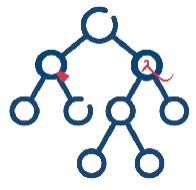
\includegraphics[height=1.0cm]{msca_logo.png}}%
    \end{center}

    \vspace{0.6cm}

    % Main title with Q logos on sides (with clickable links)
    \begin{center}
        \begin{minipage}{0.1\textwidth}
            \centering
            \href{https://quantlet.com}{
\includegraphics[height=1.1cm]{ql_logo.png}}
        \end{minipage}%
        \begin{minipage}{0.78\textwidth}
            \centering
            {\LARGE\bfseries\usebeamercolor[fg]{title}\inserttitle}

            \vspace{0.3cm}

            {\usebeamerfont{subtitle}\usebeamercolor[fg]{title}\insertsubtitle}
        \end{minipage}%
        \begin{minipage}{0.1\textwidth}
            \centering
            \href{https://quantinar.com}{
\includegraphics[height=1.1cm]{qr_logo.png}}
        \end{minipage}
    \end{center}

    \vspace{0.6cm}

    % Authors (left aligned)
    \hspace{0.5cm}{\usebeamerfont{author}\insertauthor}

    \vspace{0.3cm}

    % Institute/Affiliations (left aligned)
    \hspace{0.5cm}\begin{minipage}[t]{0.9\textwidth}
        \raggedright\small\insertinstitute
    \end{minipage}
}

%=============================================================================
% THEOREM ENVIRONMENTS
%=============================================================================
\theoremstyle{definition}
\setbeamertemplate{theorems}[numbered]
\ifdefined\atslang
\newtheorem{defn}{Definiție}
\newtheorem{thm}{Teoremă}
\newtheorem{prop}{Propoziție}
\newtheorem{rmk}{Observație}
\else
\newtheorem{defn}{Definition}
\newtheorem{thm}{Theorem}
\newtheorem{prop}{Proposition}
\newtheorem{rmk}{Remark}
\fi

%=============================================================================
% CENTRED MINIPAGE (no extra vertical space)
%=============================================================================
\newenvironment{cminipage}[1]{%
    \par\noindent\hfill\begin{minipage}{#1}\ignorespaces
}{%
    \end{minipage}\hfill\null\par
}

%=============================================================================
% CUSTOM COMMANDS
%=============================================================================
\newcommand{\E}{\mathbb{E}}
\newcommand{\Var}{\text{Var}}
\newcommand{\Cov}{\text{Cov}}
\newcommand{\Corr}{\text{Corr}}
\newcommand{\R}{\mathbb{R}}
\newcommand{\N}{\mathbb{N}}
\newcommand{\Z}{\mathbb{Z}}
\newcommand{\B}{\mathbf{B}}
\newcommand{\imark}{\textcolor{MainBlue}{\textbullet}}
\newcommand{\RMSE}{\text{RMSE}}
\newcommand{\MAE}{\text{MAE}}
\newcommand{\MAPE}{\text{MAPE}}

% Boldface vector/matrix commands (VAR, VECM, state space)
\newcommand{\bY}{\mathbf{Y}}
\newcommand{\bX}{\mathbf{X}}
\newcommand{\bA}{\mathbf{A}}
\newcommand{\bB}{\mathbf{B}}
\newcommand{\bepsilon}{\boldsymbol{\varepsilon}}
\newcommand{\bSigma}{\boldsymbol{\Sigma}}
\newcommand{\bPhi}{\boldsymbol{\Phi}}
\newcommand{\bGamma}{\boldsymbol{\Gamma}}
\newcommand{\bPi}{\boldsymbol{\Pi}}
\newcommand{\bc}{\mathbf{c}}
\newcommand{\balpha}{\boldsymbol{\alpha}}
\newcommand{\bbeta}{\boldsymbol{\beta}}
\newcommand{\bvarepsilon}{\boldsymbol{\varepsilon}}

% Seminar marks
\newcommand{\correct}{\textcolor{Forest}{\checkmark}}
\newcommand{\incorrect}{\textcolor{Crimson}{\texttimes}}
 se definește
%   \newcommand{\coursename}{Advanced Time Series Analysis and Forecasting}          (EN)
%   \newcommand{\coursename}{Analiza avansată a seriilor de timp și previziune}       (RO)  și  \def\atslang{ro}
% Fișierele .tex se află în EN/Courses, EN/Seminars, RO/Cursuri, RO/Seminarii (două niveluri sub rădăcină).
% Deck-urile sînt generate de latex/build_chapterN.py / build_seminarN.py (vezi latex/ats_build.py).

\documentclass[9pt, aspectratio=169, t]{beamer}
\providecommand{\coursename}{Advanced Time Series Analysis and Forecasting}

% Ensure content fits on slides
\setbeamersize{text margin left=8mm, text margin right=8mm}
% Smaller institute font (title page)
\setbeamerfont{institute}{size=\footnotesize}

%=============================================================================
% THEME AND STYLE CONFIGURATION
%=============================================================================
\usetheme{default}
% Using default theme for clean header/footer control

% Color Palette (matching Redispatch PDF)
\definecolor{MainBlue}{RGB}{26, 58, 110}
\definecolor{AccentBlue}{RGB}{26, 58, 110}
\definecolor{IDAred}{RGB}{205, 0, 0}
\definecolor{DarkGray}{RGB}{51, 51, 51}
\definecolor{MediumGray}{RGB}{128, 128, 128}
\definecolor{LightGray}{RGB}{248, 248, 248}
\definecolor{VeryLightGray}{RGB}{235, 235, 235}
\definecolor{KeynoteGray}{RGB}{218, 218, 218}
\definecolor{SectionGray}{RGB}{120, 120, 120}
\definecolor{FooterGray}{RGB}{100, 100, 100}
\definecolor{Crimson}{RGB}{220, 53, 69}
\definecolor{Forest}{RGB}{46, 125, 50}
\definecolor{Amber}{RGB}{181, 133, 63}
\definecolor{Orange}{RGB}{230, 126, 34}
\definecolor{Purple}{RGB}{142, 68, 173}

% Gradient background (exact Keynote 315° gradient: white to RGB 218,218,218)
\setbeamertemplate{background}{%
    \begin{tikzpicture}[remember picture, overlay]
        \shade[shading=axis, shading angle=315,
        top color=white, bottom color=KeynoteGray]
        (current page.south west) rectangle (current page.north east);
    \end{tikzpicture}%
}
% Fallback solid color for compatibility
\setbeamercolor{background canvas}{bg=}

\setbeamercolor{palette primary}{bg=MainBlue, fg=white}
\setbeamercolor{palette secondary}{bg=MainBlue!85, fg=white}
\setbeamercolor{palette tertiary}{bg=MainBlue!70, fg=white}
\setbeamercolor{structure}{fg=MainBlue}
\setbeamercolor{title}{fg=IDAred}
\setbeamercolor{frametitle}{fg=IDAred, bg=}
\setbeamercolor{block title}{bg=MainBlue, fg=white}
\setbeamercolor{block body}{bg=VeryLightGray, fg=DarkGray}
\setbeamercolor{block title alerted}{bg=Crimson, fg=white}
\setbeamercolor{block body alerted}{bg=Crimson!8, fg=DarkGray}
\setbeamercolor{block title example}{bg=Forest, fg=white}
\setbeamercolor{block body example}{bg=Forest!8, fg=DarkGray}
\setbeamercolor{item}{fg=MainBlue}

% Footer colors (override Madrid theme blue)
\setbeamercolor{author in head/foot}{fg=FooterGray, bg=}
\setbeamercolor{title in head/foot}{fg=FooterGray, bg=}
\setbeamercolor{date in head/foot}{fg=FooterGray, bg=}
\setbeamercolor{section in head/foot}{fg=FooterGray, bg=}
\setbeamercolor{subsection in head/foot}{fg=FooterGray, bg=}

% Bullet styles (apply everywhere including blocks)
\setbeamertemplate{itemize item}{\color{MainBlue}$\boxdot$}
\setbeamertemplate{itemize subitem}{\color{MainBlue}$\blacktriangleright$}
\setbeamertemplate{itemize subsubitem}{\color{MainBlue}\tiny$\bullet$}
\setbeamertemplate{itemize/enumerate body begin}{\normalsize}
\setbeamertemplate{itemize/enumerate subbody begin}{\normalsize}

% Item spacing - compact style
\setlength{\leftmargini}{10pt}       % Level 1: minimal indent
\setlength{\leftmarginii}{10pt}      % Level 2: minimal additional indent
% Compact list spacing (zero extra space before/after lists in blocks)
\makeatletter
\def\@listi{\leftmargin\leftmargini \topsep 0pt \parsep 0pt \itemsep 0pt}
\def\@listii{\leftmargin\leftmarginii \topsep 0pt \parsep 0pt \itemsep 0pt}
\makeatother

\setbeamertemplate{navigation symbols}{}

%=============================================================================
% CUSTOM HEADLINE
%=============================================================================
\setbeamertemplate{headline}{%
    \vskip10pt%
    \hbox to \paperwidth{%
        \hskip0.5cm%
        {\small\color{FooterGray}\renewcommand{\hyperlink}[2]{##2}\insertsectionhead}%
        \hfill%
        \textcolor{FooterGray}{\small\insertframenumber}%
        \hskip0.5cm%
    }%
    \vskip4pt%
    {\color{FooterGray}\hrule height 0.4pt}%
}

%=============================================================================
% CUSTOM FOOTER
%=============================================================================
\usepackage{fontawesome5}

\setbeamertemplate{footline}{%
    {\color{FooterGray}\hrule height 0.4pt}%
    \vskip4pt%
    \hbox to \paperwidth{%
        \hskip0.5cm%
        \textcolor{FooterGray}{\small\coursename}%
        \hfill%
        \raisebox{-0.1em}{%
            \begin{tikzpicture}[x=0.08em, y=0.08em, line width=0.4pt]
                \draw[FooterGray] (0,3) -- (1,4) -- (2,3.5) -- (3,5) -- (4,4) -- (5,6) -- (6,5.5) -- (7,4) -- (8,5) -- (9,7) -- (10,6) -- (11,5) -- (12,6.5) -- (13,8) -- (14,7) -- (15,6) -- (16,7.5) -- (17,9) -- (18,8) -- (19,7) -- (20,8.5) -- (21,10) -- (22,9) -- (23,8) -- (24,9.5);
            \end{tikzpicture}%
        }%
        \hskip0.5cm%
    }%
    \vskip6pt%
}

%=============================================================================
% PACKAGES
%=============================================================================
\usepackage[utf8]{inputenc}
\DeclareUnicodeCharacter{03B1}{\ensuremath{\alpha}}
\usepackage[T1]{fontenc}
\usepackage{amsmath, amssymb, amsthm}
\usepackage{mathtools}
\usepackage{bm}
\usepackage{tikz}
\usetikzlibrary{arrows.meta, positioning, shapes, calc, decorations.pathreplacing, shadings}
\usepackage{booktabs}
\usepackage{multirow}
\usepackage{array}
\usepackage{graphicx}
\usepackage{animate}
\usepackage{hyperref}
\usepackage{colortbl}
\usepackage{listings}
\lstset{language=Python, basicstyle=\ttfamily\scriptsize, keywordstyle=\color{MainBlue}\bfseries,
  commentstyle=\color{Forest}, stringstyle=\color{Crimson}, breaklines=true,
  frame=none, backgroundcolor=\color{VeryLightGray}, xleftmargin=2mm}
\hypersetup{colorlinks=true, linkcolor=MainBlue, urlcolor=MainBlue}
\graphicspath{{../../logos/}{../../charts/}{../../photos/}}
\usepackage{xcolor}
\hfuzz=2pt  % Suppress tiny overfull warnings (<2pt)
\vfuzz=2pt  % Suppress tiny vertical overfull warnings (<2pt)

%=============================================================================
% QUANTLET COMMANDS
%   \quantlet{<displayed name>}{<url>}       (generic)
%   \atsquantlet{Ch_05}{ATS_ch5_garch}       -> https://github.com/danpele/Advanced-Time-Series/tree/main/Quantlets/Ch_05/ATS_ch5_garch
%   \qlurl{<folder>} is defined per chapter by the generator (Quantlets/Ch_NN/<folder>)
%=============================================================================
\newcommand{\atsrepo}{https://github.com/danpele/Advanced-Time-Series}
\newcommand{\atsqlbase}{https://github.com/danpele/Advanced-Time-Series/tree/main/Quantlets}
\newcommand{\quantlet}[2]{%
    \hfill\href{#2}{%
        \raisebox{-0.15em}{
\includegraphics[height=0.7em]{ql_logo.png}}%
        \textcolor{MainBlue}{\tiny\ #1}%
    }%
}
\newcommand{\atsquantlet}[2]{\quantlet{\detokenize{#2}}{\atsqlbase/#1/#2}}

%=============================================================================
% NOTEBOOKS (Google Colab)
%   \colaburl{notebooks/EN/chapter5_seminar_notebook.ipynb} -> the Colab link of a file in the ATS repo
%   \nb: the chapter notebook (each seminar deck redefines it with \renewcommand)
%=============================================================================
\newcommand{\colaburl}[1]{https://colab.research.google.com/github/danpele/Advanced-Time-Series/blob/main/#1}
\newcommand{\nb}{https://colab.research.google.com/github/danpele/Advanced-Time-Series/tree/main/notebooks/EN}
\newcommand{\nbname}{notebooks/EN}

%=============================================================================
% SLIDE HELPERS (used by the generators; the same as in MFM)
%=============================================================================
% local font size for list bodies (the preamble forces \normalsize)
\newcommand{\itemsize}[1]{\setbeamertemplate{itemize/enumerate body begin}{#1}\setbeamertemplate{itemize/enumerate subbody begin}{#1}}
\newcommand{\intitle}[1]{{\hypersetup{urlcolor=white}#1}}   % white links inside coloured title bars
\newcommand{\imgcap}[1]{{\scriptsize #1}\\[0.5mm]}          % caption under a photo
\newcommand{\imgcredit}[2]{{\tiny\color{FooterGray}\href{#1}{#2}}}   % image credit: source URL, author/licence
\newcommand{\aiprompt}[1]{{\ttfamily\color{MainBlue}#1}}     % a prompt to an AI assistant

%=============================================================================
% SEMINARS: student version by default; the instructor wrapper *_solutions.tex sets \solutionstrue
%=============================================================================
\makeatletter\@ifundefined{ifsolutions}{\expandafter\newif\csname ifsolutions\endcsname}{}\makeatother
\newcommand{\solonly}[1]{\ifsolutions #1\fi}
\newcommand{\propsub}{\ifsolutions\else\framesubtitle{\ifdefined\atslang Rezolvarea se discută la seminar\else Solution discussed in class\fi}\fi}

%=============================================================================
% APPENDIX AND CHAPTER LINKS (latex/appendix_links.py writes the calls; it also re-declares these
% macros before \begin{document}, so the decks compile with or without this preamble block)
%=============================================================================
\providecommand{\atsapplink}[3]{\hypertarget{#2}{}\hyperlink{#1}{\beamergotobutton{#3}}}
\providecommand{\atsappback}[2]{\begin{tikzpicture}[remember picture,overlay]\node[anchor=south east] at ([xshift=-3mm,yshift=7mm]current page.south east){\hyperlink{#1}{\beamerreturnbutton{#2}}};\end{tikzpicture}}
\providecommand{\atschlink}[2]{\href{#1}{#2}}
\providecommand{\atschlinkt}[2]{\href{#1}{\usebeamercolor[fg]{frametitle}#2}}

%=============================================================================
% QUANTINAR COMMAND: link către un curs Quantinar (subiecte avansate)
%=============================================================================
\newcommand{\quantinar}[2]{%
    \href{#2}{%
        \raisebox{-0.15em}{
\includegraphics[height=0.8em]{qr_logo.png}}%
        \textcolor{MainBlue}{\scriptsize\ #1}%
    }%
}

%=============================================================================
% CUSTOM TITLE PAGE
%=============================================================================
\defbeamertemplate*{title page}{hybrid}[1][]
{
    \vspace{0.2cm}
    % Logos row - top header (with clickable links)
    \begin{center}
        \href{https://www.ase.ro}{
\includegraphics[height=1.0cm]{ase_logo.png}}\hspace{0.3cm}%
        \href{https://theida.net}{
\includegraphics[height=1.0cm]{ida_logo.png}}\hspace{0.3cm}%
        \href{https://blockchain-research-center.com}{
\includegraphics[height=1.0cm]{brc_logo.png}}\hspace{0.3cm}%
        \href{https://www.ai4efin.ase.ro}{
\includegraphics[height=1.0cm]{ai4efin_logo.png}}\hspace{0.3cm}%
        \href{https://ipe.ro/new}{
\includegraphics[height=1.0cm]{acad_logo.png}}\hspace{0.3cm}%
        \href{https://www.digital-finance-msca.com}{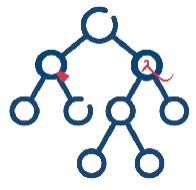
\includegraphics[height=1.0cm]{msca_logo.png}}%
    \end{center}

    \vspace{0.6cm}

    % Main title with Q logos on sides (with clickable links)
    \begin{center}
        \begin{minipage}{0.1\textwidth}
            \centering
            \href{https://quantlet.com}{
\includegraphics[height=1.1cm]{ql_logo.png}}
        \end{minipage}%
        \begin{minipage}{0.78\textwidth}
            \centering
            {\LARGE\bfseries\usebeamercolor[fg]{title}\inserttitle}

            \vspace{0.3cm}

            {\usebeamerfont{subtitle}\usebeamercolor[fg]{title}\insertsubtitle}
        \end{minipage}%
        \begin{minipage}{0.1\textwidth}
            \centering
            \href{https://quantinar.com}{
\includegraphics[height=1.1cm]{qr_logo.png}}
        \end{minipage}
    \end{center}

    \vspace{0.6cm}

    % Authors (left aligned)
    \hspace{0.5cm}{\usebeamerfont{author}\insertauthor}

    \vspace{0.3cm}

    % Institute/Affiliations (left aligned)
    \hspace{0.5cm}\begin{minipage}[t]{0.9\textwidth}
        \raggedright\small\insertinstitute
    \end{minipage}
}

%=============================================================================
% THEOREM ENVIRONMENTS
%=============================================================================
\theoremstyle{definition}
\setbeamertemplate{theorems}[numbered]
\ifdefined\atslang
\newtheorem{defn}{Definiție}
\newtheorem{thm}{Teoremă}
\newtheorem{prop}{Propoziție}
\newtheorem{rmk}{Observație}
\else
\newtheorem{defn}{Definition}
\newtheorem{thm}{Theorem}
\newtheorem{prop}{Proposition}
\newtheorem{rmk}{Remark}
\fi

%=============================================================================
% CENTRED MINIPAGE (no extra vertical space)
%=============================================================================
\newenvironment{cminipage}[1]{%
    \par\noindent\hfill\begin{minipage}{#1}\ignorespaces
}{%
    \end{minipage}\hfill\null\par
}

%=============================================================================
% CUSTOM COMMANDS
%=============================================================================
\newcommand{\E}{\mathbb{E}}
\newcommand{\Var}{\text{Var}}
\newcommand{\Cov}{\text{Cov}}
\newcommand{\Corr}{\text{Corr}}
\newcommand{\R}{\mathbb{R}}
\newcommand{\N}{\mathbb{N}}
\newcommand{\Z}{\mathbb{Z}}
\newcommand{\B}{\mathbf{B}}
\newcommand{\imark}{\textcolor{MainBlue}{\textbullet}}
\newcommand{\RMSE}{\text{RMSE}}
\newcommand{\MAE}{\text{MAE}}
\newcommand{\MAPE}{\text{MAPE}}

% Boldface vector/matrix commands (VAR, VECM, state space)
\newcommand{\bY}{\mathbf{Y}}
\newcommand{\bX}{\mathbf{X}}
\newcommand{\bA}{\mathbf{A}}
\newcommand{\bB}{\mathbf{B}}
\newcommand{\bepsilon}{\boldsymbol{\varepsilon}}
\newcommand{\bSigma}{\boldsymbol{\Sigma}}
\newcommand{\bPhi}{\boldsymbol{\Phi}}
\newcommand{\bGamma}{\boldsymbol{\Gamma}}
\newcommand{\bPi}{\boldsymbol{\Pi}}
\newcommand{\bc}{\mathbf{c}}
\newcommand{\balpha}{\boldsymbol{\alpha}}
\newcommand{\bbeta}{\boldsymbol{\beta}}
\newcommand{\bvarepsilon}{\boldsymbol{\varepsilon}}

% Seminar marks
\newcommand{\correct}{\textcolor{Forest}{\checkmark}}
\newcommand{\incorrect}{\textcolor{Crimson}{\texttimes}}


\newcommand{\qlurl}[1]{https://github.com/danpele/Advanced-Time-Series/tree/main/Quantlets/Ch_14/#1}

% Clickable citations (DOIs verified via Crossref)
\newcommand{\refAbG}{\href{https://doi.org/10.1257/000282803321455188}{Abadie și Gardeazabal (2003)}}
\newcommand{\refADHa}{\href{https://doi.org/10.1198/jasa.2009.ap08746}{Abadie, Diamond și Hainmueller (2010)}}
\newcommand{\refADHs}{\href{https://doi.org/10.18637/jss.v042.i13}{Abadie, Diamond și Hainmueller (2011)}}
\newcommand{\refADHb}{\href{https://doi.org/10.1111/ajps.12116}{Abadie, Diamond și Hainmueller (2015)}}
\newcommand{\refAba}{\href{https://doi.org/10.1257/jel.20191450}{Abadie (2021)}}
\newcommand{\refAJK}{\href{https://doi.org/10.1080/07350015.2016.1204919}{Angrist, Jordà și Kuersteiner (2018)}}
\newcommand{\refSDID}{\href{https://doi.org/10.1257/aer.20190159}{Arkhangelsky et al.\ (2021)}}
\newcommand{\refAI}{\href{https://doi.org/10.1257/jep.31.2.3}{Athey și Imbens (2017)}}
\newcommand{\refBBG}{\href{https://doi.org/10.1016/j.qref.2025.102006}{Babalos, Bouri și Gupta (2025)}}
\newcommand{\refBai}{\href{https://doi.org/10.3982/ECTA6135}{Bai (2009)}}
\newcommand{\refBBS}{\href{https://doi.org/10.1103/PhysRevLett.103.238701}{Barnett, Barrett și Seth (2009)}}
\newcommand{\refBaC}{\href{https://doi.org/10.1073/pnas.1700369114}{Baskerville și Cobey (2017)}}
\newcommand{\refASCM}{\href{https://doi.org/10.1080/01621459.2021.1929245}{Ben-Michael, Feller și Rothstein (2021)}}
\newcommand{\refBMKW}{\href{https://doi.org/10.1007/s10797-019-09566-5}{Benedek et al.\ (2020)}}
\newcommand{\refBoS}{\href{https://doi.org/10.1080/01621459.2018.1527225}{Bojinov și Shephard (2019)}}
\newcommand{\refBMSS}{\href{https://doi.org/10.1093/ej/uez020}{Born et al.\ (2019)}}
\newcommand{\refBrC}{\href{https://doi.org/10.1016/j.jeconom.2005.02.004}{Breitung și Candelon (2006)}}
\newcommand{\refCI}{\href{https://doi.org/10.1214/14-AOAS788}{Brodersen et al.\ (2015)}}
\newcommand{\refCSA}{\href{https://doi.org/10.1016/j.jeconom.2020.12.001}{Callaway și Sant’Anna (2021)}}
\newcommand{\refdCDH}{\href{https://doi.org/10.1257/aer.20181169}{de Chaisemartin și D’Haultfœuille (2020)}}
\newcommand{\refDML}{\href{https://doi.org/10.1111/ectj.12097}{Chernozhukov et al.\ (2018)}}
\newcommand{\refCWZ}{\href{https://doi.org/10.1080/01621459.2021.1920957}{Chernozhukov, Wüthrich și Zhu (2021)}}
\newcommand{\refDI}{\href{https://doi.org/10.3386/w22791}{Doudchenko și Imbens (2016)}}
\newcommand{\refDK}{\href{https://doi.org/10.1093/acprof:oso/9780199641178.001.0001}{Durbin și Koopman (2012)}}
\newcommand{\refEuroCT}{\href{https://ec.europa.eu/eurostat/databrowser/view/prc_hicp_ct/default/table}{Eurostat (2026b)}}
\newcommand{\refEuroM}{\href{https://ec.europa.eu/eurostat/web/hicp/methodology}{Eurostat (2026c)}}
\newcommand{\refFP}{\href{https://doi.org/10.3982/QE1596}{Ferman și Pinto (2021)}}
\newcommand{\refFiP}{\href{https://doi.org/10.1515/jci-2016-0026}{Firpo și Possebom (2018)}}
\newcommand{\refGew}{\href{https://doi.org/10.1080/01621459.1982.10477803}{Geweke (1982)}}
\newcommand{\refGB}{\href{https://doi.org/10.1016/j.jeconom.2021.03.014}{Goodman-Bacon (2021)}}
\newcommand{\refGra}{\href{https://doi.org/10.2307/1912791}{Granger (1969)}}
\newcommand{\refHam}{\href{https://doi.org/10.1515/9780691218632}{Hamilton (1994)}}
\newcommand{\refHar}{\href{https://doi.org/10.1017/CBO9781107049994}{Harvey (1989)}}
\newcommand{\refHCW}{\href{https://doi.org/10.1002/jae.1230}{Hsiao, Ching și Wan (2012)}}
\newcommand{\refIR}{\href{https://doi.org/10.1017/CBO9781139025751}{Imbens și Rubin (2015)}}
\newcommand{\refJor}{\href{https://doi.org/10.1257/0002828053828518}{Jordà (2005)}}
\newcommand{\refKL}{\href{https://doi.org/10.1017/9781108164818}{Kilian și Lütkepohl (2017)}}
\newcommand{\refLCG}{\href{https://doi.org/10.1093/ije/dyw098}{Lopez Bernal, Cummins și Gasparrini (2017)}}
\newcommand{\refMac}{\href{https://www.jstor.org/stable/2729691}{MacKinlay (1997)}}
\newcommand{\refMon}{\href{https://doi.org/10.1016/j.future.2016.12.009}{Mønster et al.\ (2017)}}
\newcommand{\refNW}{\href{https://doi.org/10.2307/1913610}{Newey și West (1987)}}
\newcommand{\refPea}{\href{https://doi.org/10.1017/CBO9780511803161}{Pearl (2009)}}
\newcommand{\refPMW}{\href{https://doi.org/10.3982/ECTA17813}{Plagborg-Møller și Wolf (2021)}}
\newcommand{\refRS}{\href{https://arxiv.org/abs/1903.01637}{Rambachan și Shephard (2021)}}
\newcommand{\refRSBP}{\href{https://doi.org/10.1016/j.jeconom.2023.03.008}{Roth et al.\ (2023)}}
\newcommand{\refRub}{\href{https://doi.org/10.1037/h0037350}{Rubin (1974)}}
\newcommand{\refPCMCI}{\href{https://doi.org/10.1126/sciadv.aau4996}{Runge et al.\ (2019a)}}
\newcommand{\refRunE}{\href{https://doi.org/10.1038/s41467-019-10105-3}{Runge et al.\ (2019b)}}
\newcommand{\refSch}{\href{https://doi.org/10.1103/PhysRevLett.85.461}{Schreiber (2000)}}
\newcommand{\refSV}{\href{https://doi.org/10.1504/IJMMNO.2014.059942}{Scott și Varian (2014)}}
\newcommand{\refSEC}{\href{https://www.sec.gov/files/rules/sro/nysearca/2024/34-99306.pdf}{SEC (2024)}}
\newcommand{\refSims}{\href{https://www.jstor.org/stable/1806097}{Sims (1972)}}
\newcommand{\refSGS}{\href{https://doi.org/10.7551/mitpress/1754.001.0001}{Spirtes, Glymour și Scheines (2000)}}
\newcommand{\refSW}{\href{https://doi.org/10.1111/ecoj.12593}{Stock și Watson (2018)}}
\newcommand{\refSug}{\href{https://doi.org/10.1126/science.1227079}{Sugihara et al.\ (2012)}}
\newcommand{\refSA}{\href{https://doi.org/10.1016/j.jeconom.2020.09.006}{Sun și Abraham (2021)}}
\newcommand{\refTY}{\href{https://doi.org/10.1016/0304-4076(94)01616-8}{Toda și Yamamoto (1995)}}
\newcommand{\refXu}{\href{https://doi.org/10.1017/pan.2016.2}{Xu (2017)}}
\newcommand{\refYDGS}{\href{https://doi.org/10.1038/srep14750}{Ye et al.\ (2015)}}
\newcommand{\refKPSb}{\href{https://doi.org/10.1186/s41937-017-0004-9}{Klößner et al.\ (2018)}}
\newcommand{\refFrP}{\href{https://doi.org/10.1103/PhysRevLett.99.204101}{Frenzel și Pompe (2007)}}
\newcommand{\refKSG}{\href{https://doi.org/10.1103/PhysRevE.69.066138}{Kraskov, Stögbauer și Grassberger (2004)}}
\newcommand{\refKKPS}{\href{https://doi.org/10.1080/07350015.2021.1930012}{Kaul et al.\ (2022)}}
\newcommand{\refAnd}{\href{https://doi.org/10.1111/1468-0262.00466}{Andrews (2003)}}
\newcommand{\refTak}{\href{https://doi.org/10.1007/BFb0091924}{Takens (1981)}}
\newcommand{\refADHd}{\href{https://doi.org/10.7910/DVN/24714}{Abadie, Diamond și Hainmueller (2014)}}
\newcommand{\refOECD}{\href{https://sdmx.oecd.org/public/rest/dataflow/OECD.SDD.NAD/DSD_NAMAIN1@DF_QNA/1.1}{OECD (2026)}}
\newcommand{\refEuroH}{\href{https://ec.europa.eu/eurostat/databrowser/view/prc_hicp_minr/default/table}{Eurostat (2026a)}}

\title[Analiza avansată a seriilor de timp și previziune]{Analiza avansată a seriilor de timp și previziune}
\subtitle{Capitolul 14: Inferență cauzală pentru serii de timp}
\author[D.T. Pele]{Daniel Traian PELE}
\institute{Academia de Studii Economice din București\\
IDA Institute Digital Assets\\
Blockchain Research Center\\
AI4EFin Artificial Intelligence for Energy Finance\\
Academia Română, Institutul de Prognoză Economică\\
MSCA Digital Finance}
\date{}

%=============================================================================
\providecommand{\atsapplink}[3]{\hypertarget{#2}{}\hyperlink{#1}{\beamergotobutton{#3}}}  % APPLINKS-MACROS
\providecommand{\atsappback}[2]{\begin{tikzpicture}[remember picture,overlay]\node[anchor=south east] at ([xshift=-3mm,yshift=7mm]current page.south east){\hyperlink{#1}{\beamerreturnbutton{#2}}};\end{tikzpicture}}  % APPLINKS-MACROS
\providecommand{\atschlink}[2]{\href{#1}{#2}}  % APPLINKS-MACROS
\providecommand{\atschlinkt}[2]{\href{#1}{\usebeamercolor[fg]{frametitle}#2}}  % APPLINKS-MACROS
\begin{document}
%=============================================================================

{
\setbeamertemplate{headline}{}
\setbeamertemplate{footline}{}
\begin{frame}[noframenumbering]
    \titlepage
\end{frame}
}
% BEGIN-ACRONYMS (generat de latex/acronyms.py; nu editati manual)
\begin{frame}{Acronime folosite în acest material (1/2)}
\setbeamertemplate{itemize/enumerate body begin}{\footnotesize}
\begin{columns}[T]
\begin{column}{0.49\textwidth}
\begin{itemize}\setlength{\itemsep}{0pt}
    \item \textbf{ADH}: Abadie, Diamond and Hainmueller (Abadie, Diamond și Hainmueller)
    \item \textbf{AI}: Artificial Intelligence (inteligență artificială)
    \item \textbf{AR}: AutoRegressive (model); in event studies: Abnormal Return (model autoregresiv; în studiile de eveniment: randament anormal)
    \item \textbf{BET}: Bucharest Exchange Trading (index) — indicele de referință al Bursei de Valori București
    \item \textbf{BNR}: Banca Națională a României
    \item \textbf{CAR}: Cumulative Abnormal Return (randamentul anormal cumulat)
    \item \textbf{CCM}: Convergent Cross Mapping (estimare încrucișată convergentă (Sugihara et al. 2012))
    \item \textbf{CS}: Callaway and Sant'Anna (estimator) — estimatorul Callaway și Sant'Anna
    \item \textbf{DML}: Double/Debiased Machine Learning (machine learning dublu (fără deplasare))
\end{itemize}
\end{column}
\begin{column}{0.49\textwidth}
\begin{itemize}\setlength{\itemsep}{0pt}
    \item \textbf{ECOFIN}: Economic and Financial Affairs Council (of the EU) — Consiliul Afaceri Economice și Financiare al UE
    \item \textbf{EODHD}: EOD Historical Data (market-data provider) — furnizor de date de piață
    \item \textbf{ETF}: Exchange-Traded Fund (fond tranzacționat la bursă)
    \item \textbf{HAC}: Heteroskedasticity and Autocorrelation Consistent (standard errors) — erori standard robuste la heteroscedasticitate și autocorelație
    \item \textbf{IAPC}: Indicele armonizat al prețurilor de consum
    \item \textbf{ITS}: Interrupted Time Series (serie de timp întreruptă)
    \item \textbf{LLM}: Large Language Model (model lingvistic de mari dimensiuni)
    \item \textbf{LP}: Local Projection (proiecție locală)
    \item \textbf{MCI}: Momentary Conditional Independence (independență condiționată momentană)
\end{itemize}
\end{column}
\end{columns}
\end{frame}
\begin{frame}{Acronime folosite în acest material (2/2)}
\setbeamertemplate{itemize/enumerate body begin}{\footnotesize}
\begin{columns}[T]
\begin{column}{0.49\textwidth}
\begin{itemize}\setlength{\itemsep}{0pt}
    \item \textbf{MCMC}: Markov Chain Monte Carlo (metode Monte Carlo cu lanțuri Markov)
    \item \textbf{MSPE}: Mean Squared Prediction Error (eroarea medie pătratică de prognoză)
    \item \textbf{OCDE}: Organizația pentru Cooperare și Dezvoltare Economică
    \item \textbf{OLS}: Ordinary Least Squares (metoda celor mai mici pătrate)
    \item \textbf{PC1}: first Principal Component (prima componentă principală)
    \item \textbf{PCMCI}: PC algorithm + Momentary Conditional Independence (algoritmul PC urmat de testul de independență condiționată momentană (Runge et al. 2019))
    \item \textbf{PIB}: Produsul intern brut
    \item \textbf{RMSPE}: Root Mean Squared Prediction Error (rădăcina erorii pătratice medii de predicție)
    \item \textbf{SC}: Synthetic Control (control sintetic)
    \item \textbf{SDID}: Synthetic Difference in Differences (diferența în diferențe sintetică)
\end{itemize}
\end{column}
\begin{column}{0.49\textwidth}
\begin{itemize}\setlength{\itemsep}{0pt}
    \item \textbf{SEC}: Securities and Exchange Commission (Comisia americană pentru valori mobiliare)
    \item \textbf{SUA}: Statele Unite ale Americii
    \item \textbf{SVAR}: Structural Vector AutoRegression (model vector autoregresiv structural)
    \item \textbf{TE}: Transfer Entropy (entropia de transfer)
    \item \textbf{TSA}: Time Series Analysis (Serii de timp, cursul de licență)
    \item \textbf{TVA}: Taxa pe valoarea adăugată
    \item \textbf{TWFE}: Two-Way Fixed Effects (efecte fixe bidirecționale (unitate și perioadă))
    \item \textbf{UE}: Uniunea Europeană
    \item \textbf{UE-26}: cele 26 de țări UE în afară de România
    \item \textbf{VAR}: Vector AutoRegression (model vector autoregresiv)
    \item \textbf{VIX}: CBOE Volatility IndeX (indicele de volatilitate CBOE)
\end{itemize}
\end{column}
\end{columns}
\end{frame}
% END-ACRONYMS

\begin{frame}{Întrebarea de azi și traseul}
\itemsize{\small}
\begin{itemize}
    \item \textbf{Întrebarea}: cînd ne spune o analiză de serii de timp \textit{ce s-ar fi întîmplat} fără un șoc sau fără o politică și cît de siguri putem fi?
    \begin{itemize}
        \item predicția nu este intervenție: o variabilă o poate prognoza pe alta fără să o cauzeze
    \end{itemize}
    \item \textbf{Traseul} capitolului
    \begin{itemize}
        \item cauzalitatea Granger, rezultate potențiale pentru serii de timp, entropia de transfer
        \item descoperirea relațiilor cauzale: PCMCI și convergent cross mapping, cu limitele lor
        \item serii de timp întrerupte și studii de eveniment cu erori dependente
        \item controlul sintetic și succesorii lui; DiD eșalonat; CausalImpact; DML
    \end{itemize}
    \item Cunoștințe necesare: Seminarul 14 și slide-ul \hyperlink{c14known}{\textcolor{MainBlue}{Cunoscut din TSA și din \atschlink{https://danpele.github.io/Advanced-Time-Series/RO/Cursuri/capitol3_modele_var_structurale_proiectii_locale.pdf}{Capitolul 3} și elemente noi}}
\end{itemize}
\end{frame}

\begin{frame}{Rezultatele învățării}
\itemsize{\small}
\begin{itemize}
    \item Distingeți cauzalitatea Granger de un efect cauzal dinamic și enunțați condițiile în care o mărime estimată din serii de timp are sens cauzal
    \item Aplicați teste Granger condiționate cu covarianță HAC, estimați entropia de transfer și citiți critic rezultatele PCMCI și convergent cross mapping
    \item Estimați efecte din serii de timp întrerupte și din studii de eveniment cu erori standard care respectă dependența serială
    \item Construiți controale sintetice (clasic, cu termen liber, augmentat, DiD sintetic), aplicați inferența prin placebo și replicați un rezultat publicat
    \item Folosiți contrafactuale în spațiul stărilor de tip CausalImpact și judecați onest ipotezele de identificare ale fiecărei metode
\end{itemize}
\end{frame}

\begin{frame}{Bibliografie, date și instrumente}
\itemsize{\small}
\begin{itemize}
    \item Cauzalitate și serii de timp: \refGra; \refSims; \refRS; \refBoS; \refAJK; \refSW
    \begin{itemize}
        \item descoperire: \refSch; \refPCMCI; \refRunE; \refSug
    \end{itemize}
    \item Evaluarea politicilor
    \begin{itemize}
        \item control sintetic: \refADHa; \refADHb; \refAba; \refASCM; \refSDID
        \item DiD eșalonat și CausalImpact: \refCSA; \refCI; sinteza \refAI
    \end{itemize}
    \item Quantlet-urile Python ale capitolului: \href{https://github.com/danpele/Advanced-Time-Series/tree/main/Quantlets/Ch_14}{Quantlets/Ch\_14}
    \begin{itemize}
        \item \texttt{numpy}, \texttt{scipy} (ponderile controlului sintetic prin programare pătratică) și \texttt{statsmodels} (spațiul stărilor); fiecare estimator este scris explicit, fără cutii negre
    \end{itemize}
    \item Notebook-ul cursului: \href{\colaburl{notebooks/EN/chapter14_lecture_notebook.ipynb}}{deschideți în Google Colab}
\end{itemize}
\end{frame}

\begin{frame}{Datele folosite în acest capitol}
\itemsize{\footnotesize}
\begin{center}
\scriptsize
\begin{tabular}{>{\raggedright\arraybackslash}p{3.3cm}>{\raggedright\arraybackslash}p{5.6cm}>{\raggedright\arraybackslash}p{3.4cm}}
\toprule
\textbf{Seria} & \textbf{Sursa, eșantionul} & \textbf{Utilizarea} \\
\midrule
Inflația IAPC, 27 de țări UE; IAPC la cote de taxare constante & \refEuroH, \refEuroCT: lunar, 2015 -- august 2026 & ITS, control sintetic pentru România \\
PIB pe locuitor, Germania de Vest și 16 țări OCDE & \refADHd: 1960--2003 & replicarea ADH (2015) \\
PIB real, Regatul Unit și 23 de țări OCDE & \refOECD: trimestrial, 1995--2019 & dublura Brexit \\
Prețuri zilnice ale indicilor și criptoactivelor; EUR/RON & EODHD; cursul de referință BNR; pînă la 18 septembrie 2026 & Granger, PCMCI, studiu de eveniment, CausalImpact \\
\bottomrule
\end{tabular}
\end{center}
\end{frame}

\begin{frame}{Două limbaje ale cauzalității}
\itemsize{\small}
\begin{columns}[T]
\begin{column}{0.36\textwidth}
\centering

\includegraphics[height=0.28\textheight]{ch14_pearl_2013.jpg}\\[1mm]
\imgcap{Judea Pearl, Premiul Turing 2011}
\imgcredit{https://commons.wikimedia.org/wiki/File:Judea_Pearl_at_NIPS_2013_(11781981594)_(cropped).jpg}{Foto: Better Than Bacon (2013); CC BY 2.0; Wikimedia Commons}\\[1mm]\centering
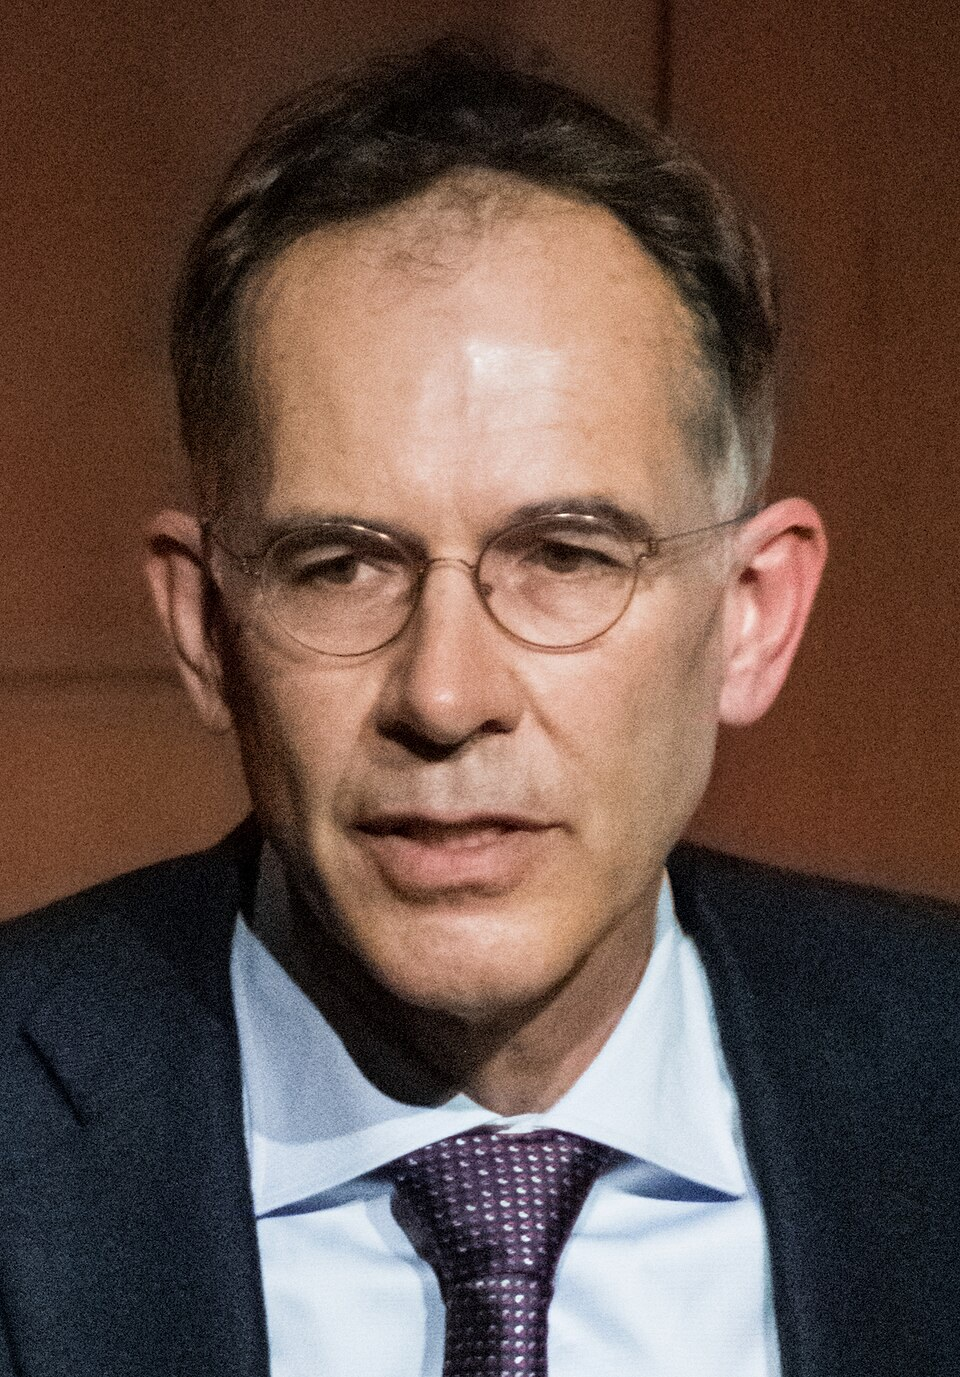
\includegraphics[height=0.20\textheight]{ch14_imbens_2022.jpg}\\[1mm]
\imgcap{Guido Imbens, Premiul Nobel pentru economie 2021}
\imgcredit{https://commons.wikimedia.org/wiki/File:Guido_Imbens_Lemley_Lecture_1_(cropped).jpg}{Foto: Filetime (2022); CC0; Wikimedia Commons}
\end{column}
\begin{column}{0.62\textwidth}
\begin{itemize}
    \item \textbf{Modele cauzale structurale} \refPea
    \begin{itemize}
        \item grafuri și operatorul $do(\cdot)$: $do(X = x)$ fixează $X$ prin intervenție, în loc să îl observe
        \item condiții în care un efect cauzal este identificat din date observaționale
    \end{itemize}
    \item \textbf{Rezultate potențiale} \refRub, \refIR
    \begin{itemize}
        \item $Y(1)$, $Y(0)$: rezultatele unei unități cu și fără tratament; doar unul dintre ele este observat
        \item mecanisme de alocare; designul înaintea analizei
    \end{itemize}
    \item \textbf{Seriile de timp} adaugă ordinea, dependența și o singură realizare
    \begin{itemize}
        \item o țară, o istorie, un singur drum al tratamentului
        \item Granger și PCMCI vorbesc limbajul grafurilor; controlul sintetic, DiD și CausalImpact vorbesc limbajul rezultatelor potențiale
    \end{itemize}
\end{itemize}
\end{column}
\end{columns}
\end{frame}

\begin{frame}{Patru studii de caz}
\itemsize{\footnotesize}
\begin{center}
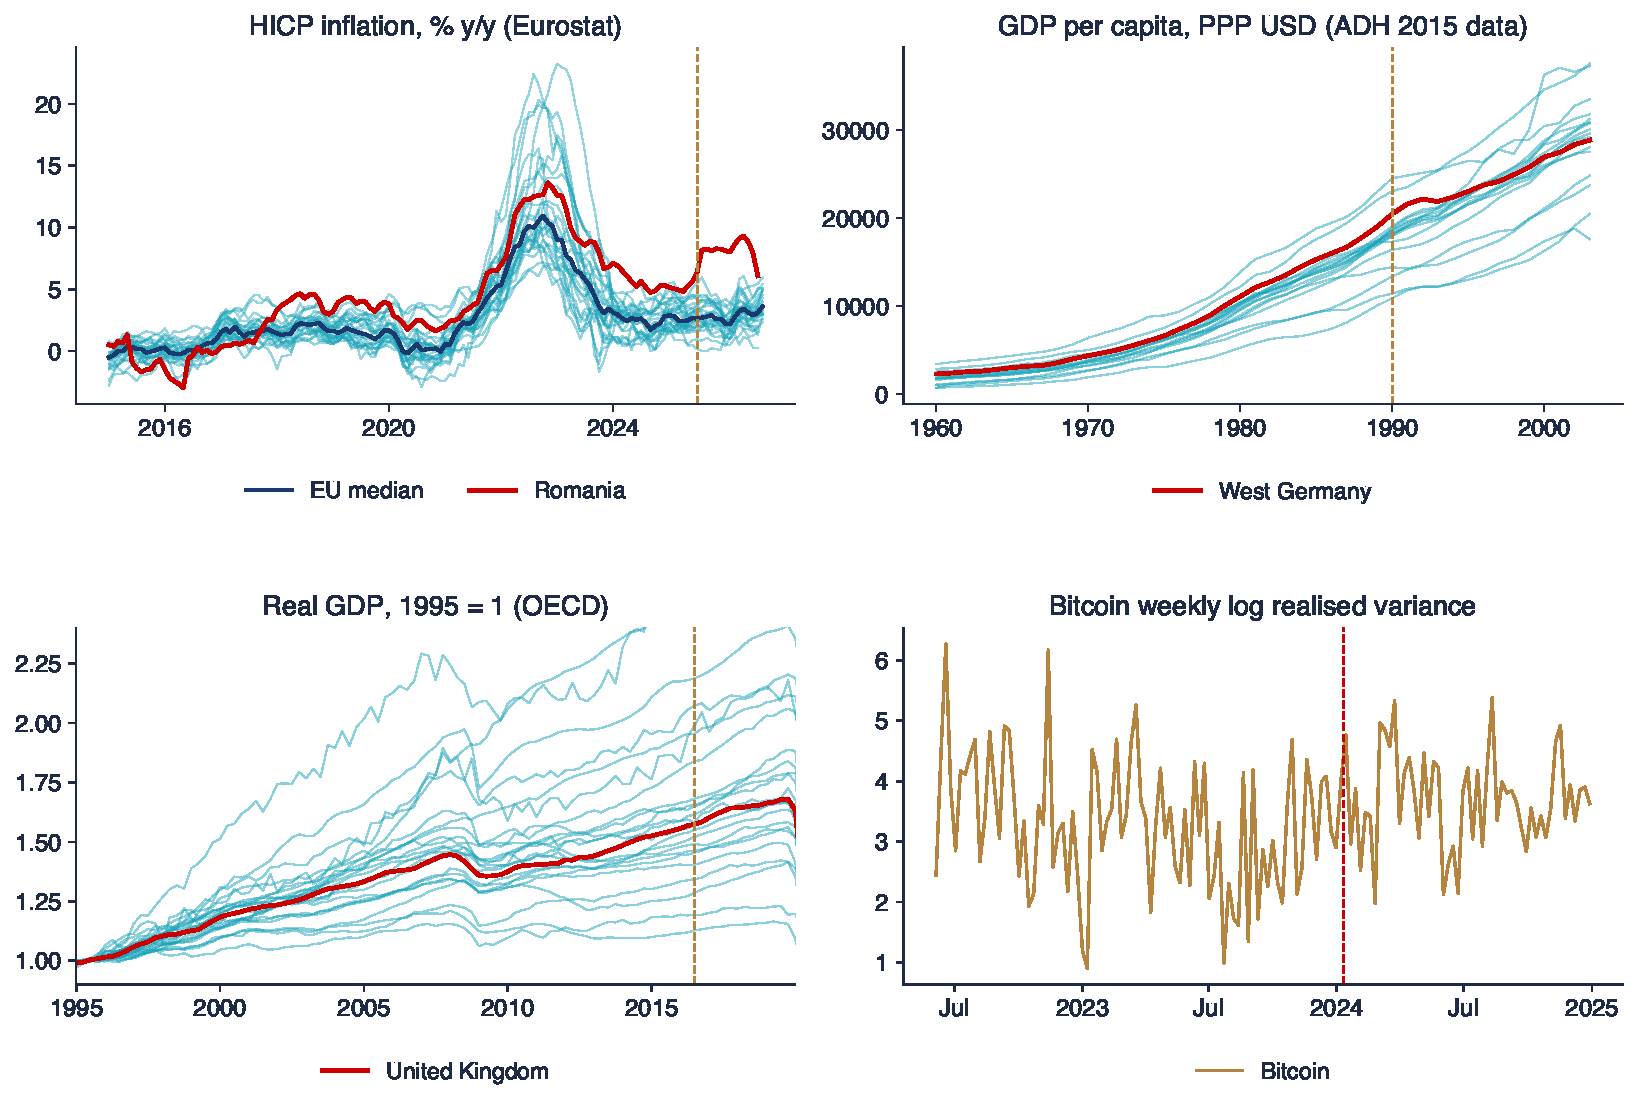
\includegraphics[width=0.97\textwidth,height=0.66\textheight,keepaspectratio]{ats_ch14_overview.pdf}
\end{center}
\vspace{-0.25cm}
\begin{itemize}
    \item Inflația României față de 26 de țări UE; Germania de Vest față de eșantionul OCDE; PIB-ul real al Regatului Unit față de 23 de țări OCDE; varianța realizată a Bitcoin în jurul aprobării ETF-urilor spot
\end{itemize}
\quantlet{ATS\_ch14\_romania}{\qlurl{ATS_ch14_romania}}
\end{frame}

\begin{frame}{Interpretarea celor patru studii de caz}
\itemsize{\small}
\begin{itemize}
    \item România: inflația IAPC anuală 5{,}6\% în iunie 2025, 8{,}2\% în august 2025, maximum 9{,}3\% în mai 2026; 6{,}1\% în august 2026 (mediana UE 3{,}1\%)
    \item Fiecare caz are o singură unitate tratată și un grup de unități netratate sau de serii de control observate pe o perioadă lungă înainte: designul studiului de caz comparativ
    \item România se află în afara intervalului donatorilor înaintea tratamentului (cea mai mare inflație din UE): un avertisment pentru orice metodă care interpolează
    \item Volatilitatea Bitcoin este zgomotoasă, iar seriile de control sînt slabe: cadrul în care o analiză onestă poate să nu găsească nimic
\end{itemize}
\end{frame}


%=============================================================================
\section{Cauzalitatea Granger și efectele cauzale}
%=============================================================================

\begin{frame}{Cunoscut din TSA și din \atschlinkt{https://danpele.github.io/Advanced-Time-Series/RO/Cursuri/capitol3_modele_var_structurale_proiectii_locale.pdf}{Capitolul 3} și elemente noi}
\itemsize{\small}
\begin{itemize}
    \item \hypertarget{c14known}{}Cunoscut: testul Granger bivariat într-un VAR (\atschlink{https://danpele.github.io/Time-Series-Analysis/RO/Cursuri/capitol6_modele_var_cauzalitate_granger.pdf}{TSA, Capitolul 6}); identificarea SVAR, proiecțiile locale și proxy SVAR (\atschlink{https://danpele.github.io/Advanced-Time-Series/RO/Cursuri/capitol3_modele_var_structurale_proiectii_locale.pdf}{Capitolul 3}); HAC (\atschlink{https://danpele.github.io/Advanced-Time-Series/RO/Cursuri/capitol0_recapitulare_inferenta.pdf}{Capitolul 0}); filtrul Kalman și BSTS (\atschlink{https://danpele.github.io/Advanced-Time-Series/RO/Cursuri/capitol6_modele_spatiul_starilor_filtrare_bayesiana.pdf}{Capitolul 6})
    \item Nou: ce pot și ce nu pot spune aceste instrumente despre intervenții
    \begin{itemize}
        \item rezultate potențiale pentru serii de timp; non-anticipare; cînd un răspuns la impuls este un efect cauzal
        \item descoperire neliniară și pe grafuri; studii de caz comparative cu o singură unitate tratată
    \end{itemize}
    \item Replicări: Abadie, Diamond și Hainmueller (2015, tabelul 1, figurile 2--5); Born et al.\ (2019, tabelul 2, figura 2); Sugihara et al.\ (2012, figura 3)
\end{itemize}
\end{frame}

\begin{frame}{Cauzalitatea Granger: definiția (1/2)}
\itemsize{\small}
\begin{itemize}
    \item \refGra: $x$ \textbf{cauzează în sens Granger} pe $y$ dacă trecutul lui $x$ reduce eroarea pătratică medie a celei mai bune prognoze la un pas a lui $y$ \[ \E\big[(y_{t+1} - \E[y_{t+1}\mid \mathcal I_t])^2\big] < \E\big[(y_{t+1} - \E[y_{t+1}\mid \mathcal I_t\setminus x])^2\big] \]
    \begin{itemize}
        \item $\mathcal I_t$: toată informația disponibilă pînă la $t$; $\mathcal I_t\setminus x$: aceeași informație, fără trecutul lui $x$
        \item $\E[y_{t+1}\mid\cdot]$: media condiționată, adică cea mai bună prognoză în sensul erorii pătratice medii
    \end{itemize}
    \item În practică, $\mathcal I_t$ este o mulțime finită de laguri dintr-o regresie \[ y_t = c + \sum_{j=1}^p a_jy_{t-j} + \sum_{j=1}^p b_jx_{t-j} + \sum_{j=1}^p \gamma_j'z_{t-j} + u_t \]
    \begin{itemize}
        \item $p$: numărul de laguri; $a_j$, $b_j$: coeficienții lagurilor lui $y$ și ale lui $x$; $z_t$: un vector de alte serii de condiționare, cu vectorii de coeficienți $\gamma_j$; $u_t$: eroarea
        \item ipoteza nulă de non-cauzalitate Granger: $H_0$: $b_1 = \dots = b_p = 0$
    \end{itemize}
\end{itemize}
\end{frame}

\begin{frame}{Cauzalitatea Granger: definiția (2/2)}
\itemsize{\small}
\begin{itemize}
    \item \textbf{Statistica Wald}: o formă pătratică a coeficienților estimați ai lagurilor lui $x$ \[ W = \hat b'\hat V_b^{-1}\hat b \;\to\; \chi^2_p \quad \text{sub} \ H_0 \]
    \begin{itemize}
        \item $\hat b = (\hat b_1, \dots, \hat b_p)'$; $\hat V_b$: matricea ei de covarianță estimată; $H_0$ se respinge pentru un $W$ mare (p-value mic)
        \item $\hat V_b$ HAC (\atschlink{https://danpele.github.io/Advanced-Time-Series/RO/Cursuri/capitol0_recapitulare_inferenta.pdf}{Capitolul 0}) cînd $u_t$ este heteroscedastic, ca pentru randamente \refNW
    \end{itemize}
    \item Serii integrate sau cointegrate \refTY
    \begin{itemize}
        \item se adaugă atîtea laguri suplimentare cît este ordinul maxim de integrare și se testează doar primele $p$ laguri
    \end{itemize}
    \item \textbf{Intensitatea}: măsura Geweke \refGew, care se poate descompune pe frecvențe \refBrC{} (\atschlink{https://danpele.github.io/Advanced-Time-Series/RO/Cursuri/capitol11_analiza_spectrala_analiza_wavelet.pdf}{Capitolul 11}) \[ F_{x\to y} = \ln\big(\sigma^2_{\mathrm{restrîns}}/\sigma^2_{\mathrm{complet}}\big) \]
    \begin{itemize}
        \item $\sigma^2_{\mathrm{restrîns}}$, $\sigma^2_{\mathrm{complet}}$: varianțele reziduale ale regresiei fără și cu lagurile lui $x$; $F_{x\to y} \ge 0$, iar 0 înseamnă absența cauzalității Granger
    \end{itemize}
\end{itemize}
\end{frame}

\begin{frame}{Cauzalitatea Granger privește predicția}
\itemsize{\small}
\begin{columns}[T]
\begin{column}{0.36\textwidth}
\centering
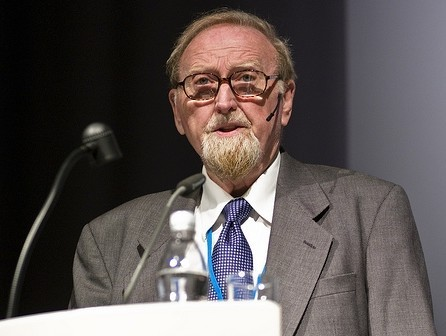
\includegraphics[height=0.44\textheight]{ch1_granger_2008.jpg}\\[1mm]
\imgcap{Clive Granger, Premiul Nobel pentru economie 2003}
\imgcredit{https://commons.wikimedia.org/wiki/File:Clive_Granger_by_Olaf_Storbeck.jpg}{Foto: Olaf Storbeck (2008); CC BY-SA 2.0; Wikimedia Commons}
\end{column}
\begin{column}{0.62\textwidth}
\begin{itemize}
    \item Patru moduri în care $x$ cauzează în sens Granger pe $y$ fără să îl cauzeze
    \begin{itemize}
        \item \textbf{un factor comun} $z$, omis, care ajunge la $x$ și la $y$ cu laguri diferite
        \item \textbf{anticipări}: prețurile activelor se mișcă înaintea evenimentelor anticipate (acțiunile „cauzează” PIB-ul; \refSims)
        \item \textbf{momentul observării}: ore de închidere diferite, agregarea și eșantionarea transformă legături instantanee în legături cu lag
        \item \textbf{erori de măsurare} în $y$, pe care $x$ ajută să le filtreze
    \end{itemize}
    \item Și invers: un efect real poate fi invizibil pentru test
    \begin{itemize}
        \item neliniar, contemporan sau compensat de reacția politicii
    \end{itemize}
\end{itemize}
\end{column}
\end{columns}
\end{frame}

\begin{frame}{Un factor comun creează cauzalitate Granger}
\itemsize{\footnotesize}
\begin{center}
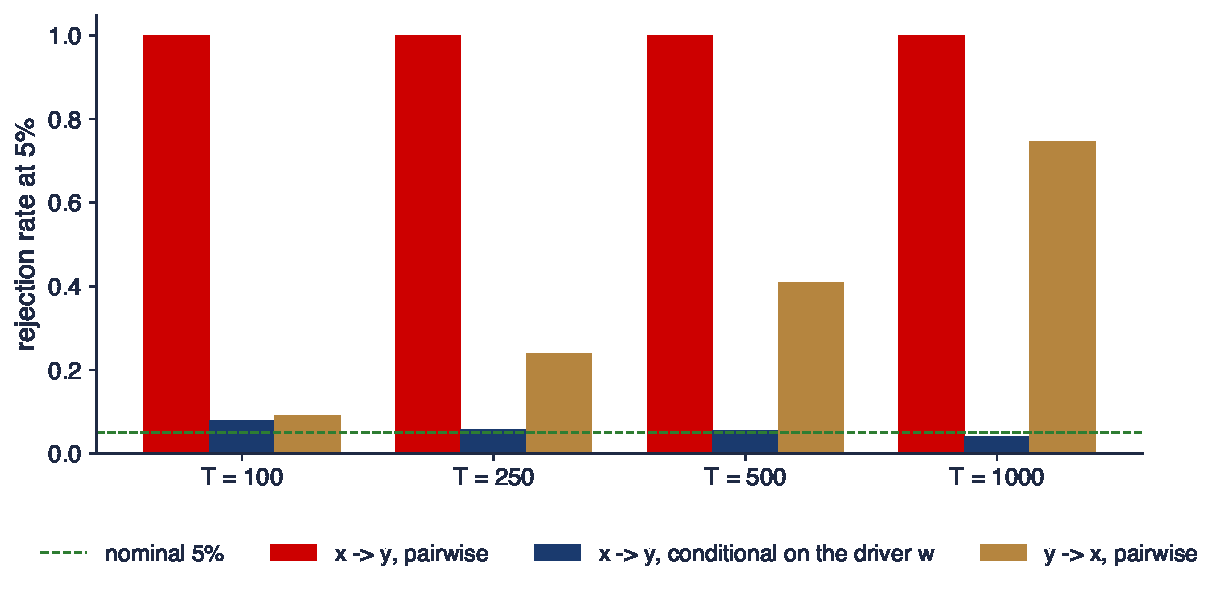
\includegraphics[width=0.97\textwidth,height=0.59\textheight,keepaspectratio]{ats_ch14_granger_sim.pdf}
\end{center}
\vspace{-0.25cm}
\begin{itemize}
    \item Sistem simulat: un factor $w_t = 0{,}9w_{t-1} + \eta_t$ (AR(1), $\phi = 0{,}9$); $x_t = w_{t-1} + e_t$, $y_t = w_{t-3} + u_t$; $\eta_t, e_t, u_t$: zgomot independent
    \item $x$ nu are niciun efect asupra lui $y$; teste cu $p = 2$ laguri (pe perechi) și $p = 4$ (condiționat de $w$), 500 de repetări
\end{itemize}
\quantlet{ATS\_ch14\_granger}{\qlurl{ATS_ch14_granger}}
\end{frame}

\begin{frame}{Interpretarea experimentului cu factor comun}
\itemsize{\small}
\begin{itemize}
    \item Pe perechi, $x$ „cauzează în sens Granger” pe $y$ în 100\% din eșantioane încă de la $T = 100$: $x$ aduce informație despre $w$ cu două perioade înaintea lui $y$
    \item Condiționat de factorul comun, rata de respingere scade la nivelul nominal (4\% la $T = 1000$): cauzalitatea Granger este relativă la mulțimea de informație
    \item Testul invers respinge și el tot mai des (9\% la $T = 100$, 75\% la $T = 1000$): trecutul lui $y$ este și el informativ despre factorul persistent
    \item Eșantioanele mai mari fac o concluzie falsă mai sigură, nu mai puțin sigură: puterea nu înseamnă validitate
\end{itemize}
\end{frame}

\begin{frame}{Relații lead--lag între New York, Frankfurt și București}
\itemsize{\footnotesize}
\begin{center}
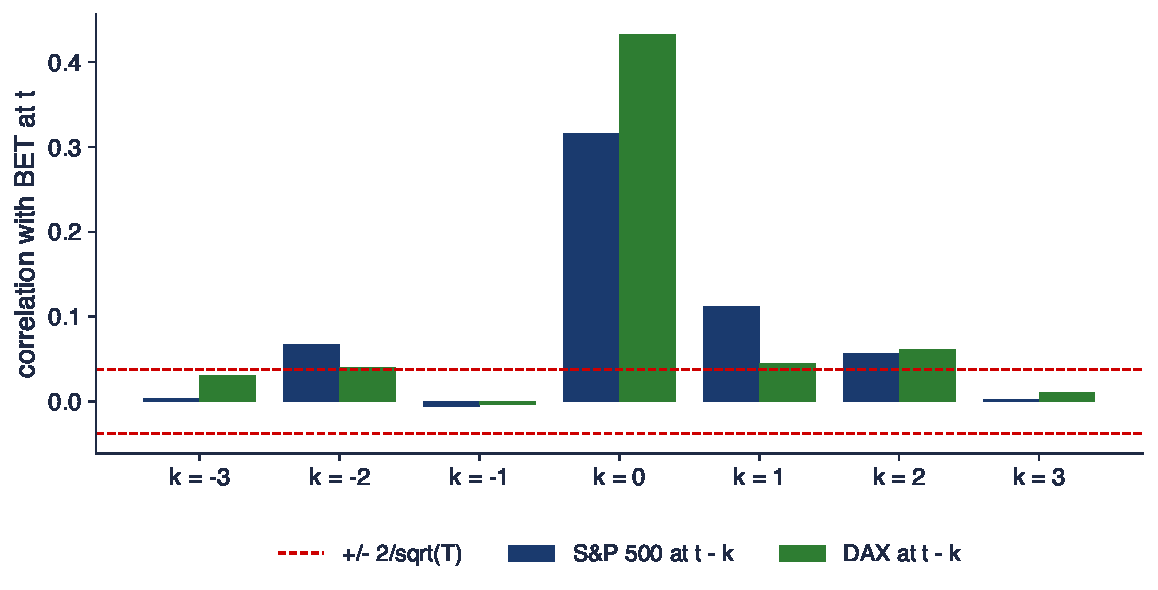
\includegraphics[width=0.97\textwidth,height=0.65\textheight,keepaspectratio]{ats_ch14_granger_markets.pdf}
\end{center}
\vspace{-0.25cm}
\begin{itemize}
    \item Randamente logaritmice zilnice, zile comune de tranzacționare 6 ianuarie 2015 -- 18 septembrie 2026 ($T = 2\,815$); corelația BET la $t$ cu S\&P 500 și DAX la $t - k$
\end{itemize}
\quantlet{ATS\_ch14\_granger}{\qlurl{ATS_ch14_granger}}
\end{frame}

\begin{frame}{Teste Granger pe cei trei indici}
\itemsize{\small}
\begin{center}
\footnotesize
\begin{tabular}{lccc}
\toprule
\textbf{Ipoteza} ($p = 2$) & \textbf{Wald (HAC)} & \textbf{p-value} & \textbf{condiționare} \\
\midrule
S\&P 500 $\not\to$ BET & 15{,}3 & $<$0{,}001 & -- \\
BET $\not\to$ S\&P 500 & 4{,}5 & 0{,}105 & -- \\
S\&P 500 $\not\to$ BET & 9{,}9 & 0{,}007 & DAX \\
DAX $\not\to$ BET & 1{,}6 & 0{,}449 & -- \\
S\&P 500 $\not\to$ DAX & 18{,}3 & $<$0{,}001 & -- \\
\bottomrule
\end{tabular}
\end{center}
\begin{itemize}
    \item Statistica Wald clasică (fără HAC) pentru S\&P 500 $\to$ BET este 34{,}3: ignorarea heteroscedasticității ar dubla în mod artificial dovezile
    \item Interpretare: New York se închide după București și Frankfurt; corelația la lagul 1 (0{,}11) este informație sosită după închiderea Bucureștiului, nu un efect al prețurilor americane asupra firmelor românești
    \item DAX, care se închide odată cu Bucureștiul, are corelație contemporană (0{,}43) și niciun efect cu lag: momentul observării creează rezultatul Granger
\end{itemize}
\end{frame}

\begin{frame}{Rezultate potențiale pentru serii de timp (1/2)}
\itemsize{\small}
\begin{itemize}
    \item \textbf{Traiectoria tratamentului}: șirul tratamentelor (sau al șocurilor) $w_{1:T} = (w_1, \dots, w_T)$ \refRS, \refBoS
    \begin{itemize}
        \item $w_t$: tratamentul la $t$, binar (politica aplicată sau nu) sau continuu (mărimea unui șoc)
    \end{itemize}
    \item \textbf{Rezultatul potențial} $Y_t(w_{1:T})$: valoarea pe care ar avea-o $Y_t$ dacă traiectoria tratamentului ar fi $w_{1:T}$
    \begin{itemize}
        \item se observă doar rezultatul potențial al traiectoriei care a avut loc efectiv
    \end{itemize}
    \item \textbf{Non-anticiparea}: rezultatul de azi depinde doar de tratamentele de pînă azi \[ Y_t(w_{1:T}) = Y_t(w_{1:t}) \]
    \begin{itemize}
        \item anunțurile o încalcă, dacă anunțul însuși nu este definit ca tratament
    \end{itemize}
\end{itemize}
\end{frame}

\begin{frame}{Rezultate potențiale pentru serii de timp (2/2)}
\itemsize{\small}
\begin{itemize}
    \item \textbf{Efectul cauzal dinamic} la orizontul $h$: modificarea lui $Y_{t+h}$ cînd se schimbă doar tratamentul de la $t$, din $w'$ în $w$ \[ \tau_{t,h} = Y_{t+h}(w_{1:t-1}, w, w_{t+1:t+h}) - Y_{t+h}(w_{1:t-1}, w', w_{t+1:t+h}) \]
    \begin{itemize}
        \item tratamentele anterioare $w_{1:t-1}$ și cele ulterioare $w_{t+1:t+h}$ sînt menținute fixe
        \item se observă o singură istorie: doar mediile în timp (sau pe unități) ale lui $\tau_{t,h}$ sînt estimabile
    \end{itemize}
    \item \refRS: presupunem că $w_t$ este \textbf{secvențial la fel de bun ca aleator}, adică independent de rezultatele potențiale, condiționat de trecut
    \begin{itemize}
        \item atunci răspunsul la impuls și coeficientul proiecției locale sînt medii ponderate ale lui $\tau_{t,h}$, fără a presupune liniaritatea
    \end{itemize}
    \item Partea dificilă nu este niciodată regresia, ci afirmația că șocul nu poate fi prezis din rezultatele potențiale
\end{itemize}
\end{frame}

\begin{frame}{Identificarea efectelor cauzale dinamice în macroeconomie}
\itemsize{\small}
\begin{itemize}
    \item \textbf{Șocuri narative și de înaltă frecvență} ca instrumente: proiecții locale \refJor{} și proxy SVAR \refSW{} (\atschlink{https://danpele.github.io/Advanced-Time-Series/RO/Cursuri/capitol3_modele_var_structurale_proiectii_locale.pdf}{Capitolul 3})
    \begin{itemize}
        \item instrumentul trebuie să fie relevant, exogen contemporan și necorelat cu valorile anterioare și viitoare ale celorlalte șocuri \refSW
    \end{itemize}
    \item \textbf{Scoruri de propensitate pentru politică}: \refAJK{} modelează decizia Fed pe baza prognozelor pe care le avea și reponderează rezultatele (ponderare prin inversul probabilității)
    \begin{itemize}
        \item identificare prin selecție pe variabile observate: mulțimea de informație a Fed este observată prin Greenbook
    \end{itemize}
    \item \textbf{Experimente pe serii de timp}: \refBoS{} dau teste exacte de randomizare pentru o unitate tratată la momente aleatoare (experimente de tranzacționare)
    \item Proiecțiile locale și VAR estimează aceleași răspunsuri în populație \refPMW: alegerea privește deplasarea și varianța, nu identificarea
\end{itemize}
\end{frame}

\begin{frame}{Entropia de transfer (1/2)}
\itemsize{\small}
\begin{itemize}
    \item \refSch: informația pe care trecutul lui $x$ o adaugă despre $y_t$, dincolo de trecutul lui $y$ \[ TE_{x\to y} = I\big(y_t;\, x_{t-1}^{(l)} \mid y_{t-1}^{(k)}\big) = \E\Big[\ln\dfrac{p(y_t\mid y^{(k)}_{t-1}, x^{(l)}_{t-1})}{p(y_t\mid y^{(k)}_{t-1})}\Big] \ge 0 \]
    \item Notațiile
    \begin{itemize}
        \item $y^{(k)}_{t-1} = (y_{t-1}, \dots, y_{t-k})$: ultimele $k$ valori ale lui $y$; $x^{(l)}_{t-1}$: ultimele $l$ valori ale lui $x$
        \item $p(\cdot\mid\cdot)$: o densitate condiționată; $I(A; B\mid C)$: informația mutuală condiționată a lui $A$ și $B$, dat $C$, în nats (logaritm natural)
    \end{itemize}
    \item $TE_{x\to y} = 0$ dacă și numai dacă $x$ nu adaugă nimic distribuției predictive a lui $y$
    \begin{itemize}
        \item non-cauzalitate Granger în distribuție, nu doar în medie
    \end{itemize}
\end{itemize}
\end{frame}

\begin{frame}{Entropia de transfer (2/2)}
\itemsize{\small}
\begin{itemize}
    \item \textbf{Cazul gaussian} \refBBS: entropia de transfer este jumătate din măsura Geweke, deci testul Granger liniar este un test TE \[ TE_{x\to y} = \tfrac12\ln\big(\sigma^2_{\mathrm{restrîns}}/\sigma^2_{\mathrm{complet}}\big) = \tfrac12 F_{x\to y} \]
    \begin{itemize}
        \item demonstrația în \atsapplink{atsapp2}{atssrc1}{Anexă}
    \end{itemize}
    \item \textbf{Estimarea neparametrică}: estimatori cu $k$ cei mai apropiați vecini \refKSG, \refFrP
    \begin{itemize}
        \item densitățile sînt înlocuite cu distanțele pînă la cei mai apropiați vecini în spațiul comun
        \item semnificația prin permutarea sursei pe blocuri, care păstrează autocorelația ei
    \end{itemize}
    \item Aceleași rezerve ca la Granger: un flux de informație nu este o intervenție
\end{itemize}
\end{frame}

\begin{frame}{O legătură neliniară pe care testul Granger liniar o ratează}
\itemsize{\footnotesize}
\begin{center}
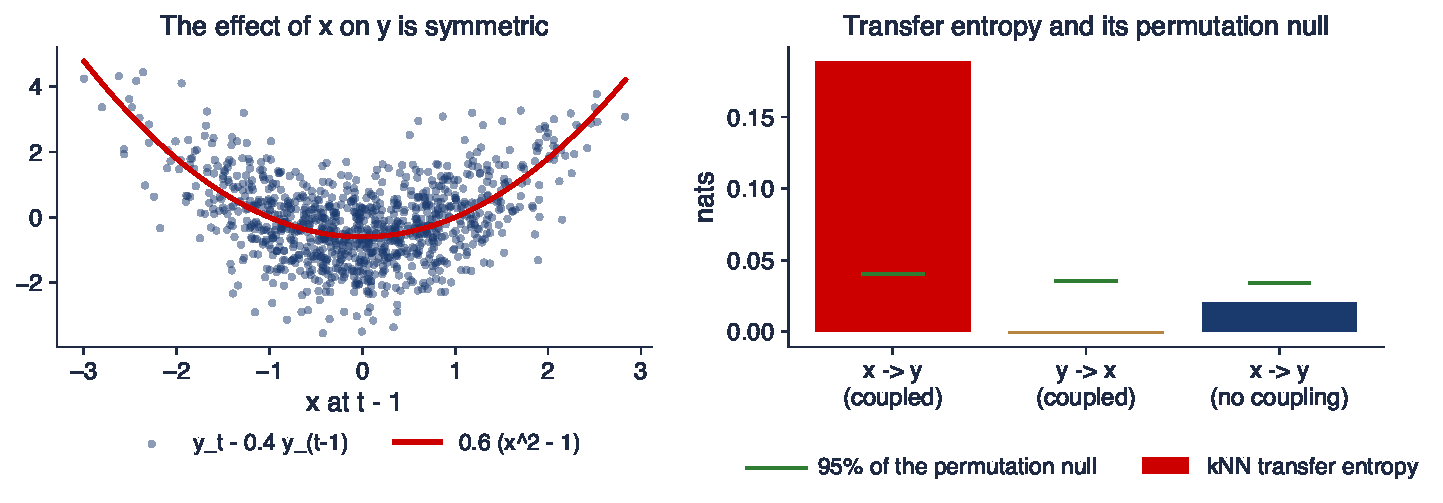
\includegraphics[width=0.97\textwidth,height=0.59\textheight,keepaspectratio]{ats_ch14_te.pdf}
\end{center}
\vspace{-0.25cm}
\begin{itemize}
    \item Simulare: $y_t = 0{,}4y_{t-1} + 0{,}6(x_{t-1}^2 - 1) + u_t$, $x$ un AR(1) gaussian cu varianța 1, $u_t$ zgomot cu distribuția Normală standard, $T = 1\,000$
    \item $x_{t-1}^2 - 1$ are media zero și nu este corelat cu $x_{t-1}$; TE kNN cu $k = 5$ vecini, 199 de permutări pe blocuri
\end{itemize}
\quantlet{ATS\_ch14\_granger}{\qlurl{ATS_ch14_granger}}
\end{frame}

\begin{frame}{Interpretarea entropiei de transfer}
\itemsize{\small}
\begin{itemize}
    \item Granger liniar: p-value 0{,}86; TE gaussiană 0{,}05$\times10^{-3}$ nats: efectul simetric se anulează în medie într-o regresie liniară
    \item TE kNN $x\to y$: 0{,}189 nats, $p$ prin permutare 0{,}005; direcția inversă \ensuremath{-}0{,}001 ($p$ 0{,}76); fără legătură 0{,}021 ($p$ 0{,}26)
    \item Pe piețele de pe slide-ul anterior, TE gaussiană de la S\&P 500 la BET este 6{,}1$\times10^{-3}$ nats: semnificativă, dar foarte mică ca informație
    \item TE cere mult mai multe date decît Granger și o alegere atentă a lui $k$, a lungimii istoriilor și a blocurilor de permutare; preînregistrați-le
\end{itemize}
\end{frame}

\begin{frame}{Recapitulare: cauzalitatea Granger și efectele cauzale}
\itemsize{\small}
\begin{itemize}
    \item Cauzalitatea Granger înseamnă predictibilitate suplimentară relativ la o mulțime de informație; lărgirea mulțimii o poate crea sau distruge
    \item Un efect cauzal cere rezultate potențiale, non-anticipare și o alocare la fel de bună ca una aleatoare, condiționat de trecut
    \item Entropia de transfer extinde Granger la distribuții; pentru procese gaussiene cele două coincid
\end{itemize}
\end{frame}


%=============================================================================
\section{Descoperirea relațiilor cauzale în serii de timp}
%=============================================================================

\begin{frame}{Grafurile seriilor de timp (1/2)}
\itemsize{\small}
\begin{itemize}
    \item \textbf{Nodurile} $X^i_t$: variabila $i$ la momentul $t$; o \textbf{săgeată} $X^i_{t-\tau}\to X^j_t$ cînd $X^i_{t-\tau}$ este o cauză directă a lui $X^j_t$, dat fiind restul trecutului \refRunE
    \begin{itemize}
        \item $\tau \ge 1$: lagul legăturii; $\tau_{\max}$: lagul maxim considerat
        \item graful este același la orice $t$ (staționaritate cauzală); săgețile merg doar înainte în timp
    \end{itemize}
    \item Trei ipoteze transformă independențele în săgeți \refSGS
    \begin{itemize}
        \item \textbf{Markov cauzal}: fiecare variabilă este independentă de non-efectele ei, dați părinții ei (cauzele directe)
        \item \textbf{fidelitatea}: nicio independență nu apare prin compensarea efectelor
        \item \textbf{suficiența cauzală}: nu există cauze comune ascunse
    \end{itemize}
\end{itemize}
\end{frame}

\begin{frame}{Grafurile seriilor de timp (2/2)}
\itemsize{\small}
\begin{itemize}
    \item Sub aceste ipoteze, o săgeată este o dependență condiționată de întregul trecut \[ X^i_{t-\tau}\to X^j_t \iff X^i_{t-\tau} \not\perp X^j_t \mid \mathbf X^-_t\setminus\{X^i_{t-\tau}\} \]
    \begin{itemize}
        \item $\perp$: independență ($\not\perp$: dependență); $\mathbf X^-_t$: toate variabilele la lagurile $1, \dots, \tau_{\max}$ înainte de $t$
        \item acesta este testul Granger condiționat complet (VAR)
    \end{itemize}
    \item Cu $N$ variabile și $\tau_{\max}$ laguri, mulțimea de condiționare are $N\tau_{\max}$ elemente
    \begin{itemize}
        \item puterea testului scade drastic în dimensiune mare: motivația pentru PCMCI
    \end{itemize}
\end{itemize}
\end{frame}

\begin{frame}{PCMCI}
\itemsize{\small}
\begin{itemize}
    \item \refPCMCI: doi pași, fiecare o succesiune de teste de independență condiționată (aici corelația parțială; sînt posibile și teste neliniare)
    \item \textbf{PC1} (selecția condițiilor), pentru fiecare $X^j_t$
    \begin{itemize}
        \item se pornește de la toți candidații cu lag; se elimină cei independenți de $X^j_t$, dați cei mai puternici $p$ dintre ceilalți, $p = 1, 2, \dots$
        \item rezultatul $\hat{\mathcal P}(X^j_t)$ este o supramulțime a părinților lui $X^j_t$
    \end{itemize}
    \item \textbf{MCI} (independența condiționată momentană): fiecare legătură se testează dați părinții ambelor capete \[ X^i_{t-\tau} \perp X^j_t \mid \hat{\mathcal P}(X^j_t)\setminus\{X^i_{t-\tau}\},\ \hat{\mathcal P}(X^i_{t-\tau}) \]
    \begin{itemize}
        \item condiționarea pe părinții \textbf{sursei} $X^i_{t-\tau}$ îi elimină autocorelația: rata alarmelor false rămîne aproape de $\alpha$
        \item mulțimile de condiționare rămîn mici, deci puterea se păstrează în dimensiune mare
    \end{itemize}
    \item Factorii de confuzie ascunși, legăturile contemporane, nestaționaritatea și erorile de măsurare anulează garanțiile; rezultatul este o ipoteză despre un graf
\end{itemize}
\end{frame}

\begin{frame}{PCMCI față de corelație și VAR complet}
\itemsize{\footnotesize}
\begin{center}
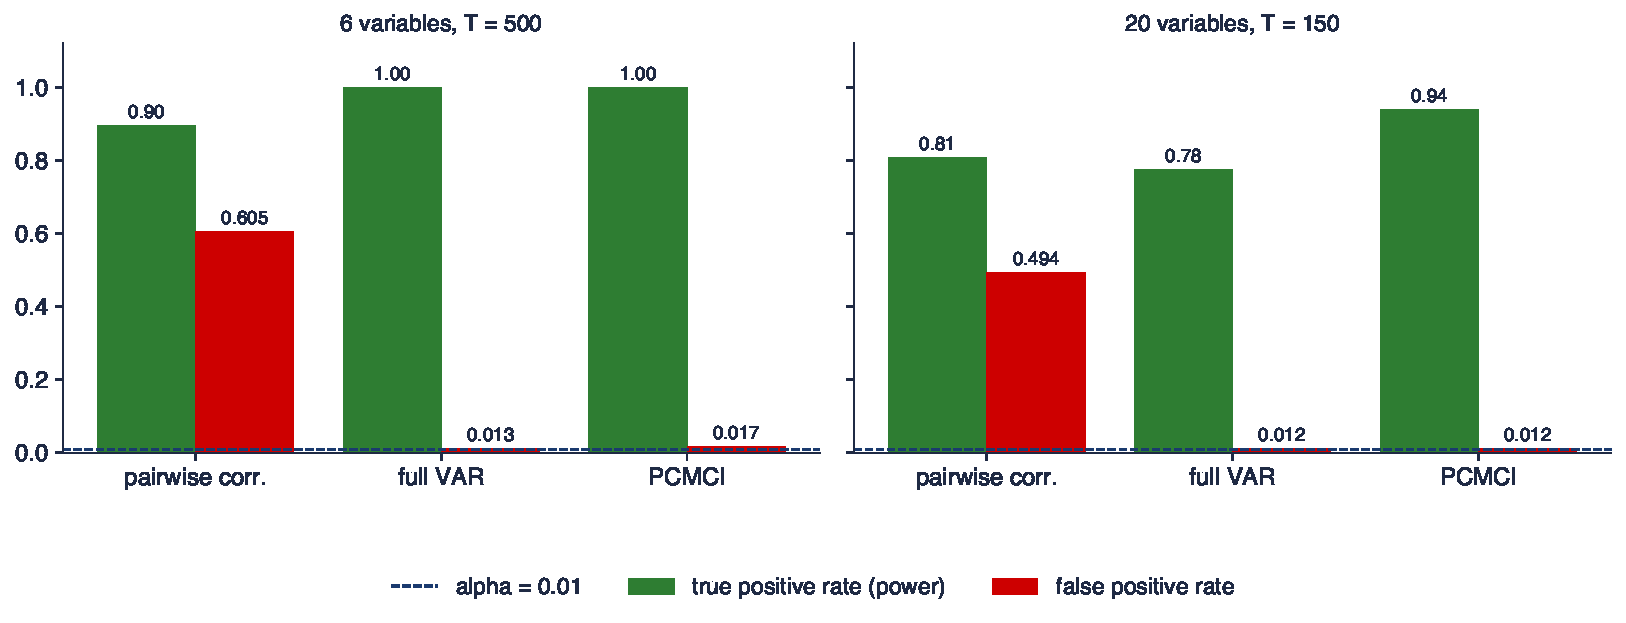
\includegraphics[width=0.97\textwidth,height=0.65\textheight,keepaspectratio]{ats_ch14_pcmci_sim.pdf}
\end{center}
\vspace{-0.25cm}
\begin{itemize}
    \item Un sistem cunoscut cu laguri (un factor comun persistent, lanțuri și un colizor), $\tau_{\max} = 3$, $\alpha = 0{,}01$, 50 de repetări; dreapta: 14 serii AR(1) independente în plus
\end{itemize}
\quantlet{ATS\_ch14\_discovery}{\qlurl{ATS_ch14_discovery}}
\end{frame}

\begin{frame}{Interpretarea experimentului de descoperire}
\itemsize{\small}
\begin{itemize}
    \item Corelațiile cu lag găsesc majoritatea legăturilor reale, dar semnalează 0{,}605 dintre cele absente: autocorelația și factorul comun fac totul corelat
    \item Șase variabile, $T = 500$: VAR complet și PCMCI sînt echivalente (putere 1{,}00 și 1{,}00; alarme false 0{,}013 și 0{,}017)
    \item Douăzeci de variabile, $T = 150$: VAR condiționează pe 60 de regresori, iar puterea lui scade la 0{,}78; PCMCI păstrează 0{,}94, cu alarme false 0{,}012
    \item Avantajul PCMCI ține de dimensiunea mare; în sisteme mici un VAR bine specificat este suficient
\end{itemize}
\end{frame}

\begin{frame}{Un graf descoperit al volatilității piețelor}
\itemsize{\footnotesize}
\begin{center}
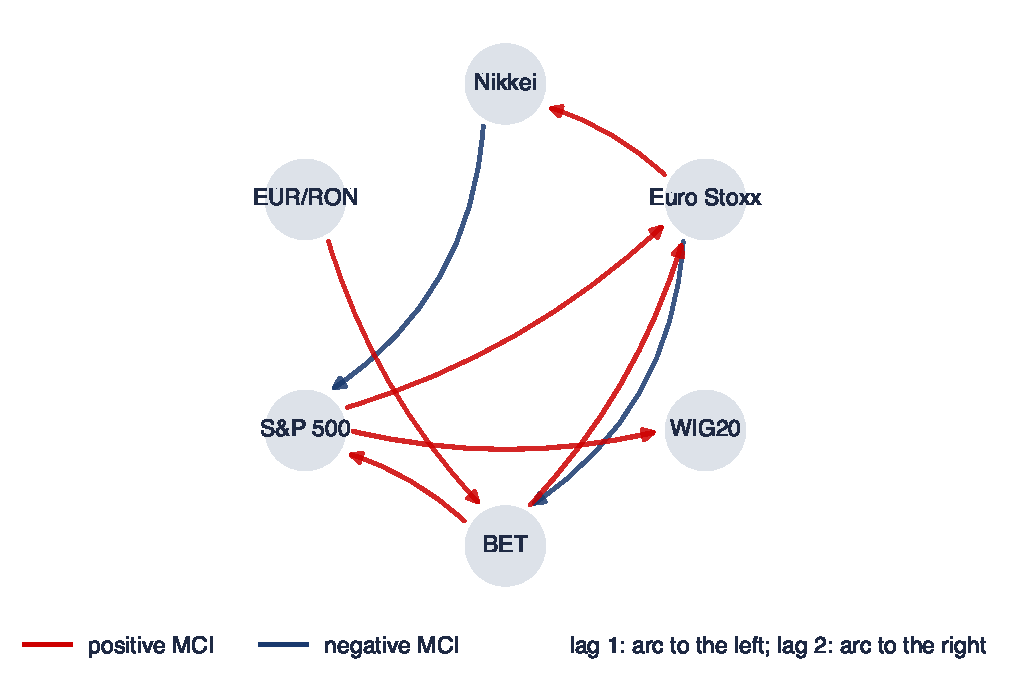
\includegraphics[width=0.97\textwidth,height=0.65\textheight,keepaspectratio]{ats_ch14_pcmci_vol.pdf}
\end{center}
\vspace{-0.25cm}
\begin{itemize}
    \item PCMCI pe logaritmul varianțelor realizate săptămînale (suma pătratelor randamentelor zilnice), 13 ianuarie 2008 -- 20 septembrie 2026, $T = 973$ de săptămîni, $\tau_{\max} = 2$, $\alpha = 0{,}01$; săptămînile elimină ordinea închiderilor zilnice
\end{itemize}
\quantlet{ATS\_ch14\_discovery}{\qlurl{ATS_ch14_discovery}}
\end{frame}

\begin{frame}{Interpretarea grafului volatilității}
\itemsize{\small}
\begin{itemize}
    \item Testele de corelație cu lag sînt semnificative pentru 56 dintre cele 60 de legături încrucișate posibile; PCMCI păstrează 8
    \item Volatilitatea este un factor comun: cea mai mare parte a dependenței brute se explică prin propriul trecut al fiecărei piețe și prin șocul global comun din aceeași săptămînă
    \item Săgețile rămase sînt corelații parțiale mici; transmiterile contemporane din aceeași săptămînă sînt invizibile pentru o analiză doar cu laguri
    \item Un factor global ascuns (știri, VIX) încalcă suficiența cauzală: citiți graful ca pe o hartă a legăturilor predictive, nu a mecanismelor de transmitere
\end{itemize}
\end{frame}

\begin{frame}{Convergent cross mapping}
\itemsize{\footnotesize}
\begin{columns}[T]
\begin{column}{0.3\textwidth}
\centering

\includegraphics[height=0.42\textheight]{ch14_sugihara_2015.jpg}\\[1mm]
\imgcap{George Sugihara}
\imgcredit{https://commons.wikimedia.org/wiki/File:Sugihara_George.png}{Foto: J Park (2015); CC BY-SA 4.0; Wikimedia Commons}
\end{column}
\begin{column}{0.68\textwidth}
\begin{itemize}
    \item Dinamici deterministe cuplate: separabilitatea lui Granger nu mai funcționează, deoarece informația cauzei se află deja în efect \refSug
    \item Takens \refTak: vectorii cu întîrziere ai lui $y$ reconstruiesc atractorul întregului sistem \[ M_y = \{(y_t, y_{t-\tau}, \dots, y_{t-(E-1)\tau})\} \]
    \begin{itemize}
        \item $E$: dimensiunea de scufundare; $\tau$: întîrzierea dintre coordonate
    \end{itemize}
    \item Dacă $x$ îl influențează pe $y$, vecinii unui punct de pe $M_y$ identifică $x_t$: se \textbf{estimează încrucișat} $x$ din $M_y$
    \begin{itemize}
        \item proiecția simplex: o medie ponderată a lui $x$ în cei $E + 1$ vecini cei mai apropiați; abilitatea: corelația $\rho$ dintre estimație și valoarea reală
    \end{itemize}
    \item Criteriul: abilitatea trebuie să \textbf{conveargă} (să crească) cu dimensiunea bibliotecii $L$, numărul de puncte folosite pentru $M_y$
    \item Atenție la direcție: abilitatea $M_y \to x$ este dovadă pentru $x \to y$
\end{itemize}
\end{column}
\end{columns}
\end{frame}

\begin{frame}{Estimarea încrucișată: o cuplare și un factor periodic comun}
\itemsize{\footnotesize}
\begin{center}
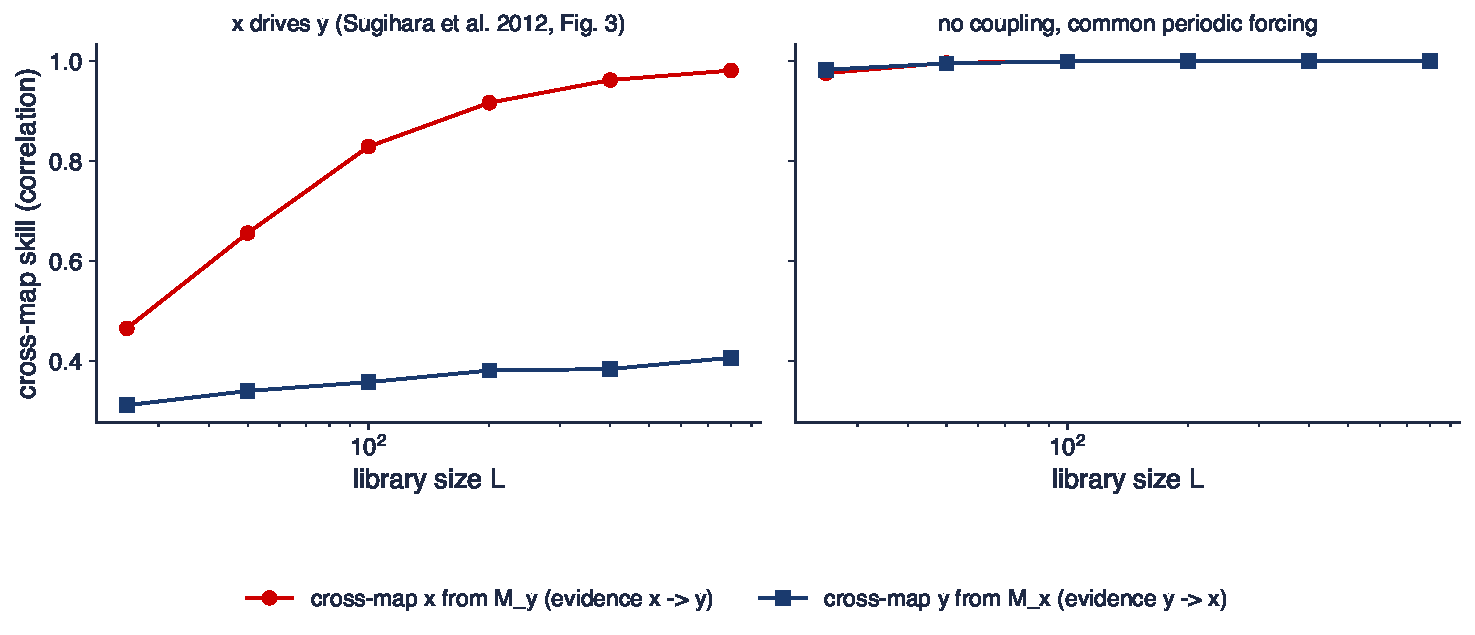
\includegraphics[width=0.97\textwidth,height=0.59\textheight,keepaspectratio]{ats_ch14_ccm.pdf}
\end{center}
\vspace{-0.25cm}
\begin{itemize}
    \item Aplicațiile logistice cuplate din \refSug: $x_{t+1} = x_t(r_x - r_xx_t - \beta_{xy}y_t)$, $y_{t+1} = y_t(r_y - r_yy_t - \beta_{yx}x_t)$
    \item $r_x = 3{,}8$, $r_y = 3{,}5$: ratele de creștere (regim haotic); $\beta_{yx} = 0{,}32$: efectul lui $x$ asupra lui $y$; $\beta_{xy} = 0$: niciun efect al lui $y$ asupra lui $x$; dreapta: două aplicații necuplate cu același factor periodic; $E = 2$
\end{itemize}
\quantlet{ATS\_ch14\_discovery}{\qlurl{ATS_ch14_discovery}}
\end{frame}

\begin{frame}{Interpretarea estimării încrucișate}
\itemsize{\small}
\begin{itemize}
    \item Stînga: abilitatea pentru $x\to y$ crește de la 0{,}47 ($L = 25$) la 0{,}98 ($L = 800$); direcția inversă rămîne în jur de 0{,}41: tiparul publicat
    \item Dreapta: nicio cuplare, totuși ambele direcții ajung la 0{,}999 și 0{,}999: un factor periodic comun sincronizează aplicațiile, iar CCM raportează cauzalitate în ambele sensuri
    \item Critici cunoscute: sezonalitate și sincronizare \refBaC, zgomot și factori externi \refMon, alegerea lagului \refYDGS
    \item Folosiți CCM pentru sisteme neliniare cu zgomot redus, cu teste pe serii surogat care păstrează sezonalitatea; niciodată ca detector automat de cauzalitate pentru serii economice
\end{itemize}
\end{frame}

\begin{frame}{Recapitulare: descoperirea relațiilor cauzale}
\itemsize{\small}
\begin{itemize}
    \item Un graf descoperit este la fel de bun ca ipotezele Markov cauzal, fidelitate și suficiență; factorii comuni ascunși sînt regula în economie
    \item PCMCI controlează alarmele false sub autocorelație și păstrează puterea în dimensiune mare
    \item CCM vizează cuplarea deterministă; sincronizarea și factorii comuni produc legături false în ambele sensuri
\end{itemize}
\end{frame}


%=============================================================================
\section{Serii de timp întrerupte și studii de eveniment}
%=============================================================================

\begin{frame}{Serii de timp întrerupte (1/2)}
\itemsize{\small}
\begin{itemize}
    \item O singură serie, o intervenție la $T_0$ \refLCG; pasul 1: se modelează perioada anterioară \[ y_t = f(t, \text{sezon}, x_t; \theta) + u_t, \qquad t \le T_0 \]
    \begin{itemize}
        \item $f$: trendul, efectele sezoniere și covariatele $x_t$, cu parametrii $\theta$; $u_t$: eroarea
    \end{itemize}
    \item Pasul 2: efectul este diferența dintre rezultat și modelul extrapolat \[ \hat\tau_t = y_t - f(t, \cdot\,; \hat\theta), \qquad t > T_0 \]
    \begin{itemize}
        \item regresia segmentată este cazul particular cu variabile dummy de nivel și de pantă după $T_0$
    \end{itemize}
    \item \textbf{Identificarea}
    \begin{itemize}
        \item nimic altceva nu se schimbă la $T_0$; modelul perioadei anterioare ar fi continuat; nicio anticipare
    \end{itemize}
\end{itemize}
\end{frame}

\begin{frame}{Serii de timp întrerupte (2/2)}
\itemsize{\small}
\begin{itemize}
    \item \textbf{Inferența cu erori dependente}: varianța efectului cumulat pe $n$ perioade \[ \mathrm{Var}\Big(\sum_{t=T_0+1}^{T_0+n}\hat\tau_t\Big) \approx n\,\Omega + a'\hat V_\theta a \]
    \begin{itemize}
        \item $\Omega$: varianța pe termen lung a lui $u_t$ (\atschlink{https://danpele.github.io/Advanced-Time-Series/RO/Cursuri/capitol0_recapitulare_inferenta.pdf}{Capitolul 0}); $\hat V_\theta$: covarianța lui $\hat\theta$; $a$: suma regresorilor lui $f$ pe cele $n$ perioade
        \item primul termen: zgomotul rezultatelor; al doilea: eroarea de estimare a contrafactualului
    \end{itemize}
    \item Cu erori AR(1), autocorelația $\rho$ și $\sigma^2 = \mathrm{Var}(u_t)$ \[ \Omega = \sigma^2\,\frac{1 + \rho}{1 - \rho} \]
    \begin{itemize}
        \item erorile standard i.i.d.\ sînt prea mici cu factorul $\sqrt{(1 + \rho)/(1 - \rho)}$, de exemplu 1,7 pentru $\rho = 0{,}5$
    \end{itemize}
\end{itemize}
\end{frame}

\begin{frame}{România 2025: două măsuri la o lună distanță}
\itemsize{\small}
\begin{columns}[T]
\begin{column}{0.4\textwidth}
\centering
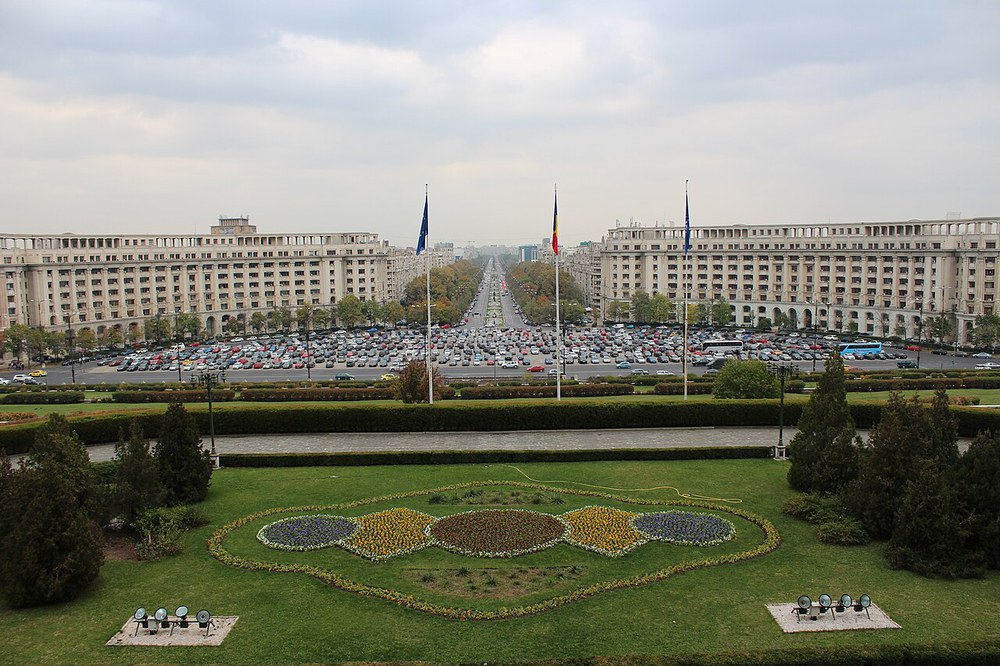
\includegraphics[height=0.40\textheight]{ch14_parliament_bucharest_2017.jpg}\\[1mm]
\imgcap{Palatul Parlamentului, București}
\imgcredit{https://commons.wikimedia.org/wiki/File:Palace_of_the_Parliament_in_Bucharest_(51878975552).jpg}{Foto: William John Gauthier (2017); CC BY-SA 2.0; Wikimedia Commons}
\end{column}
\begin{column}{0.58\textwidth}
\begin{itemize}
    \item \textbf{1 iulie 2025}
    \begin{itemize}
        \item se încheie plafonarea prețului electricității pentru gospodării (în vigoare din 2022)
        \item plafonarea prețului gazelor continuă
    \end{itemize}
    \item \textbf{7 iulie 2025}
    \begin{itemize}
        \item guvernul își asumă răspunderea în Parlament pentru un pachet fiscal (Legea 141/2025, publicată pe 25 iulie)
    \end{itemize}
    \item \textbf{1 august 2025}
    \begin{itemize}
        \item cota standard de TVA 19\% $\to$ 21\%; cotele reduse 5\% și 9\% $\to$ 11\%; accize majorate
    \end{itemize}
    \item Momentul singur nu le poate separa; IAPC la cote de taxare constante poate izola partea fiscală
    \item Întrebarea: cît au adăugat cele două măsuri la inflația din România în anul următor?
\end{itemize}
\end{column}
\end{columns}
\end{frame}

\begin{frame}{O serie de timp întreruptă pentru inflația României}
\itemsize{\footnotesize}
\begin{center}
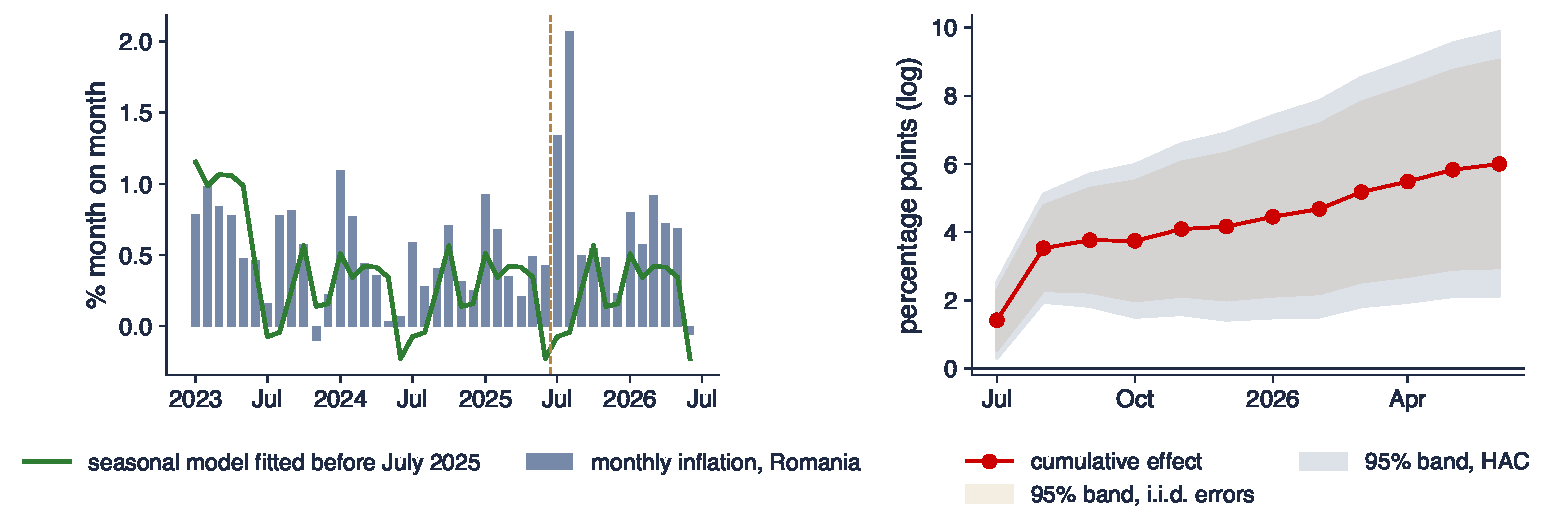
\includegraphics[width=0.97\textwidth,height=0.63\textheight,keepaspectratio]{ats_ch14_its.pdf}
\end{center}
\vspace{-0.25cm}
\begin{itemize}
    \item Inflația IAPC lunară (variația logaritmică); modelul perioadei anterioare: 12 efecte lunare și o treaptă pentru iulie 2021 -- iunie 2023, estimat pe 126 de luni pînă în iunie 2025; efectele iulie 2025 -- iunie 2026
\end{itemize}
\quantlet{ATS\_ch14\_its\_event}{\qlurl{ATS_ch14_its_event}}
\end{frame}

\begin{frame}{Interpretarea seriei de timp întrerupte}
\itemsize{\small}
\begin{itemize}
    \item Iulie 2025: +1{,}41 pp peste norma sezonieră; august 2025: +2{,}11 pp; lunile următoare, în medie +0{,}25 pp
    \item Efectul cumulat pe douăsprezece luni 6{,}0 pp; eroarea standard 1{,}55 cu erori i.i.d., 1{,}98 cu HAC (autocorelația reziduurilor 0{,}33, varianța pe termen lung de 1{,}63 ori $\sigma^2$)
    \item Contrafactualul ITS este norma sezonieră proprie a României: ignoră tot ce s-a mai întîmplat în Europa după iunie 2025
    \item Pentru a elimina șocurile comune este nevoie de un grup de control: controlul sintetic din secțiunea 5 folosește 26 de țări UE
\end{itemize}
\end{frame}

\begin{frame}{Studii de eveniment cu erori dependente}
\itemsize{\small}
\begin{itemize}
    \item \refMac, \textbf{modelul de piață} estimat pe zilele $[-250, -11]$ dinaintea evenimentului \[ r_t = \alpha + \beta r^m_t + \varepsilon_t, \qquad AR_t = r_t - \hat\alpha - \hat\beta r^m_t, \qquad CAR[0, k] = \sum_{t=0}^k AR_t \]
    \begin{itemize}
        \item $r_t$: randamentul activului; $r^m_t$: randamentul pieței; $AR_t$: randamentul anormal; $CAR[0, k]$: randamentul anormal cumulat pe zilele 0--$k$
    \end{itemize}
    \item Varianța CAR
    \begin{itemize}
        \item $(k + 1)\sigma^2$ sub erori i.i.d.; $(k + 1)\Omega$ cu corelație serială ($\Omega$: varianța pe termen lung)
        \item varianța indusă de eveniment și evenimentele grupate cer corecții transversale sau bootstrap
    \end{itemize}
    \item Identificarea: evenimentul este o surpriză în ziua 0 și nimic altceva nu s-a întîmplat
    \begin{itemize}
        \item știrile anticipate sînt încorporate în preț înaintea ferestrei
    \end{itemize}
    \item Aici: indicele BET față de Euro Stoxx 50, patru evenimente politice și fiscale din România în 2024--2025, fereastra $[0, 2]$
\end{itemize}
\end{frame}

\begin{frame}{Acțiunile românești în jurul știrilor politice și fiscale}
\itemsize{\footnotesize}
\begin{center}
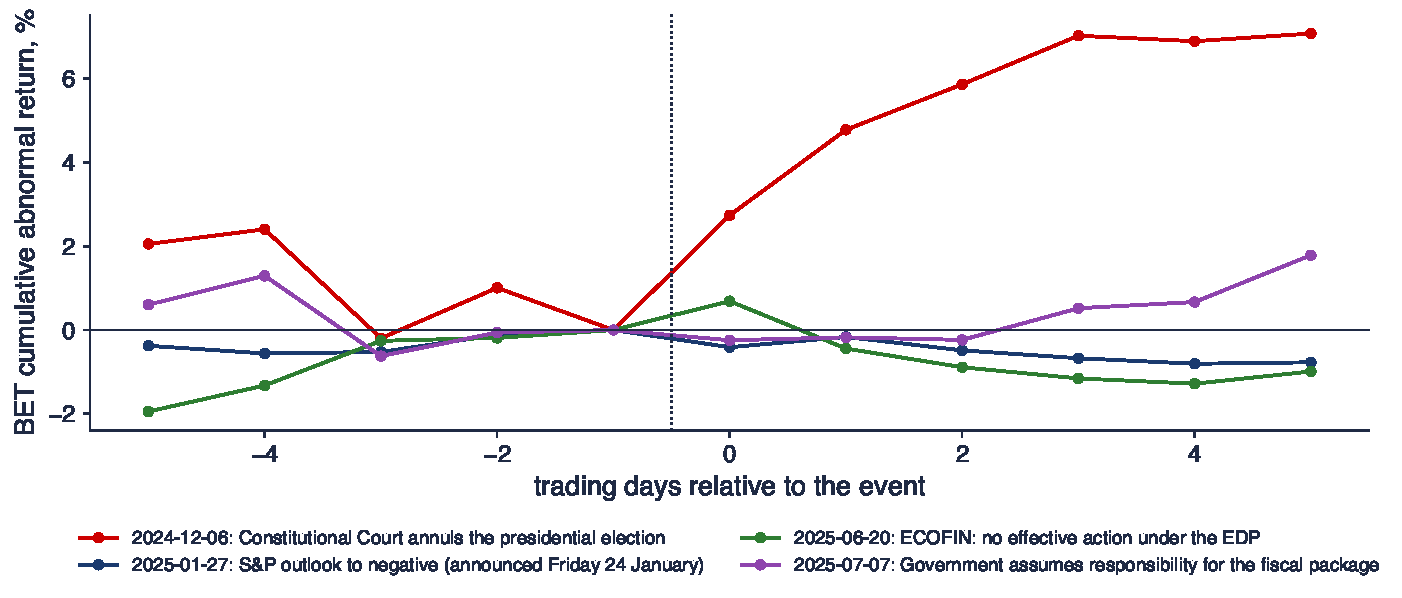
\includegraphics[width=0.97\textwidth,height=0.65\textheight,keepaspectratio]{ats_ch14_event.pdf}
\end{center}
\vspace{-0.25cm}
\begin{itemize}
    \item Randamentul anormal cumulat al BET, normalizat în ziua $-1$; modelul de piață pe Euro Stoxx 50; acțiunile de rating anunțate după închidere, într-o vineri, sînt datate în lunea următoare
\end{itemize}
\quantlet{ATS\_ch14\_its\_event}{\qlurl{ATS_ch14_its_event}}
\end{frame}

\begin{frame}{Interpretarea studiului de eveniment}
\itemsize{\small}
\begin{itemize}
    \item Anularea alegerilor prezidențiale (6 decembrie 2024): CAR[0, 2] +5{,}9\%, $t$ = 5{,}25 (i.i.d.) și 5{,}08 (HAC): piața a încorporat un risc politic mai mic
    \item Perspectiva negativă S\&P: \ensuremath{-}0{,}5\% ($t$ = \ensuremath{-}0{,}33); decizia ECOFIN: \ensuremath{-}0{,}9\% ($t$ = \ensuremath{-}0{,}52); pachetul fiscal: \ensuremath{-}0{,}2\% ($t$ = \ensuremath{-}0{,}14)
    \item Știrile fiscale erau discutate de luni de zile: nicio surpriză în ziua 0, niciun randament anormal; un rezultat nul aici nu spune nimic despre efectul economic al măsurilor
    \item Erorile standard HAC și i.i.d.\ sînt apropiate pentru randamente zilnice (autocorelație mică); diferă pentru date macro lunare (secțiunea anterioară)
\end{itemize}
\end{frame}

\begin{frame}{Recapitulare: serii de timp întrerupte și studii de eveniment}
\itemsize{\small}
\begin{itemize}
    \item ITS și studiile de eveniment compară o serie cu propriul trecut extrapolat: valide doar dacă nimic altceva nu s-a schimbat în același timp
    \item Efectele cumulate cer varianța pe termen lung a erorilor, nu $\sigma^2$
    \item Anticiparea mută efectul înaintea ferestrei: datarea știrii face parte din identificare
\end{itemize}
\end{frame}


%=============================================================================
\section{Metoda controlului sintetic}
%=============================================================================

\begin{frame}{Estimatorul controlului sintetic (1/2)}
\itemsize{\small}
\begin{itemize}
    \item Unitățile: $j = 1$ tratată, $j = 2, \dots, J + 1$ \textbf{grupul donatorilor}; tratamentul după perioada $T_0$ \refAbG, \refADHa
    \begin{itemize}
        \item $Y_{jt}(1)$, $Y_{jt}(0)$: rezultatele potențiale ale unității $j$ la $t$, cu și fără tratament
    \end{itemize}
    \item Ținta: efectul asupra unității tratate după $T_0$ \[ \tau_{1t} = Y_{1t}(1) - Y_{1t}(0), \qquad t > T_0 \]
    \begin{itemize}
        \item $Y_{1t}(1) = Y_{1t}$ este observat; $Y_{1t}(0)$ trebuie estimat
    \end{itemize}
    \item \textbf{Controlul sintetic}: o medie ponderată a donatorilor ține locul lui $Y_{1t}(0)$ \[ \hat Y_{1t}(0) = \sum_{j=2}^{J+1} w_jY_{jt}, \qquad \hat\tau_{1t} = Y_{1t} - \hat Y_{1t}(0) \]
    \begin{itemize}
        \item $w_j \ge 0$: ponderea donatorului $j$, cu $\sum_j w_j = 1$
    \end{itemize}
\end{itemize}
\end{frame}

\begin{frame}{Estimatorul controlului sintetic (2/2)}
\itemsize{\small}
\begin{itemize}
    \item \textbf{Ponderile}: combinația convexă de donatori cea mai apropiată de unitatea tratată după predictorii anteriori tratamentului \[ w^*(V) = \arg\min_w\, (X_1 - X_0w)'V(X_1 - X_0w), \qquad w_j \ge 0,\ \sum_j w_j = 1 \]
    \begin{itemize}
        \item $X_1$: vectorul predictorilor anteriori tratamentului ai unității tratate (medii ale rezultatului, covariate); $X_0$: matricea acelorași predictori pentru donatori
        \item o problemă de programare pătratică pe simplex: ponderile sînt rare și interpretabile; nicio extrapolare în afara domeniului donatorilor
    \end{itemize}
    \item $V = \mathrm{diag}(v)$: importanța fiecărui predictor
    \begin{itemize}
        \item aleasă pentru a minimiza în perioada anterioară $\mathrm{MSPE} = \frac{1}{T_0}\sum_{t \le T_0}(Y_{1t} - \sum_j w_j^*(V)Y_{jt})^2$ (optimizare imbricată, \refADHs)
        \item MSPE: eroarea pătratică medie de predicție a rezultatului; alternativa: validarea încrucișată pe o perioadă de antrenare și una de validare \refADHb
        \item cu toate rezultatele anterioare în $X$, covariatele nu primesc nicio pondere \refKKPS
    \end{itemize}
\end{itemize}
\end{frame}

\begin{frame}{Fundamentul: modelul factorial}
\itemsize{\small}
\begin{itemize}
    \item \refADHa: rezultatele fără tratament urmează un model factorial (efecte fixe interactive \refBai) \[ Y_{jt}(0) = \delta_t + \theta_tZ_j + \lambda_t\mu_j + \varepsilon_{jt} \]
    \begin{itemize}
        \item $\delta_t$: un efect comun al perioadei; $Z_j$: covariate observate, cu coeficienții variabili în timp $\theta_t$; $\lambda_t$: factori comuni neobservați; $\mu_j$: încărcările neobservate ale unității $j$; $\varepsilon_{jt}$: șocuri tranzitorii
        \item DiD presupune $\lambda_t$ constant (trenduri paralele); SC permite factorilor comuni să varieze în timp
    \end{itemize}
    \item Dacă ponderile reproduc unitatea tratată înainte de $T_0$, $\sum_j w_jY_{jt} = Y_{1t}$ pentru orice $t \le T_0$ și $\sum_j w_jZ_j = Z_1$, atunci
    \begin{itemize}
        \item deplasarea lui $\hat\tau_{1t}$ este mărginită de un termen care \textbf{scade cînd $T_0$ crește}, relativ la scala lui $\varepsilon$ (\atsapplink{atsapp1}{atssrc2}{Anexă})
        \item o potrivire bună pe o perioadă anterioară lungă arată că încărcările $\mu_j$ sînt reproduse
    \end{itemize}
    \item O perioadă anterioară scurtă cu potrivire perfectă poate însemna supraajustarea zgomotului: marginea este atunci slabă \refAba
\end{itemize}
\end{frame}

\begin{frame}{Condiții de aplicabilitate}
\itemsize{\small}
\begin{itemize}
    \item \textbf{Înfășurătoarea convexă} \refAba
    \begin{itemize}
        \item unitatea tratată trebuie să se afle în domeniul donatorilor; altfel nicio combinație convexă nu o reproduce
    \end{itemize}
    \item \textbf{Grupul donatorilor}
    \begin{itemize}
        \item unități cu structură asemănătoare, neafectate de tratament (fără efecte de propagare), fără șocuri mari proprii după $T_0$
    \end{itemize}
    \item \textbf{Nicio anticipare}
    \begin{itemize}
        \item efectele nu trebuie să înceapă înainte de $T_0$; mutați $T_0$ la anunț dacă este nevoie
    \end{itemize}
    \item \textbf{Perioadă anterioară lungă}, cu potrivire bună
    \begin{itemize}
        \item \textbf{deplasarea de interpolare}: un amestec de donatori foarte diferiți poate să nu semene cu unitatea tratată chiar dacă mediile coincid
    \end{itemize}
    \item Raportați
    \begin{itemize}
        \item ponderile, echilibrul predictorilor, RMSPE în perioada anterioară, distribuția placebo, omiterea pe rînd a donatorilor
    \end{itemize}
\end{itemize}
\end{frame}

\begin{frame}{Inferența cu o singură unitate tratată}
\itemsize{\small}
\begin{itemize}
    \item \textbf{Placebo în spațiu} \refADHa: tratamentul se atribuie pe rînd fiecărui donator, se reestimează și se calculează raportul \[ r_j = \mathrm{RMSPE}_{\mathrm{post}}/\mathrm{RMSPE}_{\mathrm{pre}}, \qquad \text{p-value} = \#\{j: r_j \ge r_1\}/(J + 1) \]
    \begin{itemize}
        \item RMSPE: rădăcina erorii pătratice medii de predicție a controlului sintetic, înainte (pre) și după (post) $T_0$; un $r_j$ mare: o diferență mare după tratament, relativ la potrivirea anterioară
        \item $\#\{\cdot\}$: numărul de unități; cel mai mic p-value posibil este $1/(J + 1)$; exact doar dacă tratamentul este atribuit aleator între unități, altfel o ordonare descriptivă \refFiP
    \end{itemize}
    \item \textbf{Alte verificări de robustețe}
    \begin{itemize}
        \item placebo în timp: un $T_0$ fictiv în perioada anterioară nu trebuie să dea niciun efect
        \item omiterea pe rînd: se elimină fiecare donator cu pondere pozitivă și se reestimează
    \end{itemize}
    \item \textbf{Inferența conformală} \refCWZ: se testează $H_0$: $\tau_{1t} = \tau_0$ permutînd reziduurile în timp
    \begin{itemize}
        \item permutări pe blocuri pentru dependență; intervale de încredere prin inversarea testului după $\tau_0$
    \end{itemize}
\end{itemize}
\end{frame}

\begin{frame}{Studiu de caz: costul economic al reunificării Germaniei}
\itemsize{\small}
\begin{columns}[T]
\begin{column}{0.38\textwidth}
\centering
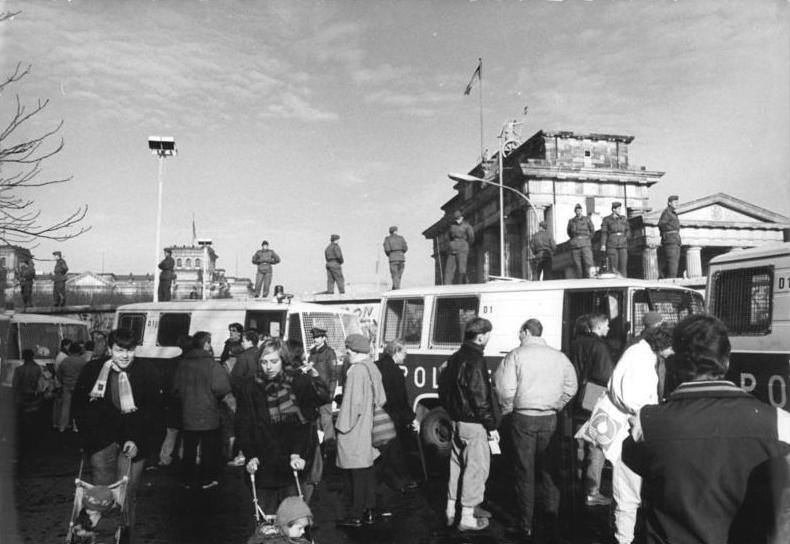
\includegraphics[height=0.42\textheight]{ch14_brandenburg_gate_1989.jpg}\\[1mm]
\imgcap{Poarta Brandenburg, Berlin, 11 noiembrie 1989}
\imgcredit{https://commons.wikimedia.org/wiki/File:Bundesarchiv_Bild_183-1989-1111-009,_Berlin,_Brandenburger_Tor,_Polizeiabsperrung.jpg}{Foto: Peer Grimm, Bundesarchiv Bild 183-1989-1111-009 (1989); CC BY-SA 3.0 de; Wikimedia Commons}
\end{column}
\begin{column}{0.6\textwidth}
\begin{itemize}
    \item \refADHb
    \begin{itemize}
        \item a scăzut reunificarea din 1990 PIB-ul pe locuitor al Germaniei de Vest?
    \end{itemize}
    \item Datele \refADHd
    \begin{itemize}
        \item Germania de Vest și 16 țări OCDE, 1960--2003
        \item predictori: PIB pe locuitor, deschiderea comercială, inflația, ponderea industriei, școlarizarea, rata investițiilor
    \end{itemize}
    \item $V$ prin validare încrucișată (secțiunea 4 și codul de replicare)
    \begin{itemize}
        \item predictori de antrenare 1971--1980, rezultate de validare 1981--1990
        \item ponderile finale din predictorii 1981--1990 cu acest $V$
    \end{itemize}
    \item Erată (2026)
    \begin{itemize}
        \item rezultatul este PIB-ul pe locuitor în USD PPC \textit{curenți}, nu în USD 2002 cum este etichetat în articol
    \end{itemize}
\end{itemize}
\end{column}
\end{columns}
\end{frame}

\begin{frame}{Replicare: ponderile și echilibrul predictorilor}
\itemsize{\small}
\begin{columns}[T]
\begin{column}{0.38\textwidth}
\begin{center}
\footnotesize
\begin{tabular}{lrr}
\toprule
\textbf{Donator} & \textbf{replicare} & \textbf{ADH, tabelul 1} \\
\midrule
Austria & 0{,}42 & 0{,}42 \\
Statele Unite & 0{,}22 & 0{,}22 \\
Japonia & 0{,}16 & 0{,}16 \\
Elveția & 0{,}11 & 0{,}11 \\
Țările de Jos & 0{,}09 & 0{,}09 \\
\bottomrule
\end{tabular}
\end{center}

\end{column}
\begin{column}{0.6\textwidth}
\begin{center}
\footnotesize
\begin{tabular}{lrrr}
\toprule
\textbf{Predictor} & \textbf{Germania de Vest} & \textbf{sintetic} & \textbf{media OCDE} \\
\midrule
PIB pe locuitor & 15809 & 15805 & 13669 \\
Deschidere comercială & 56{,}8 & 56{,}9 & 59{,}8 \\
Inflația & 2{,}6 & 3{,}5 & 7{,}6 \\
Ponderea industriei & 34{,}5 & 34{,}4 & 33{,}8 \\
Școlarizare & 55{,}5 & 55{,}3 & 38{,}7 \\
Rata investițiilor & 27{,}0 & 27{,}0 & 25{,}9 \\
\bottomrule
\end{tabular}
\end{center}

\end{column}
\end{columns}\begin{itemize}
    \item $V$ ales prin validare încrucișată și programarea pătratică reproduc ponderile publicate cu două zecimale; toți ceilalți donatori primesc pondere zero
    \item Media simplă OCDE diferă la fiecare predictor: comparația neponderată ar fi deplasată
\end{itemize}
\end{frame}

\begin{frame}{Germania de Vest și controlul ei sintetic}
\itemsize{\footnotesize}
\begin{center}
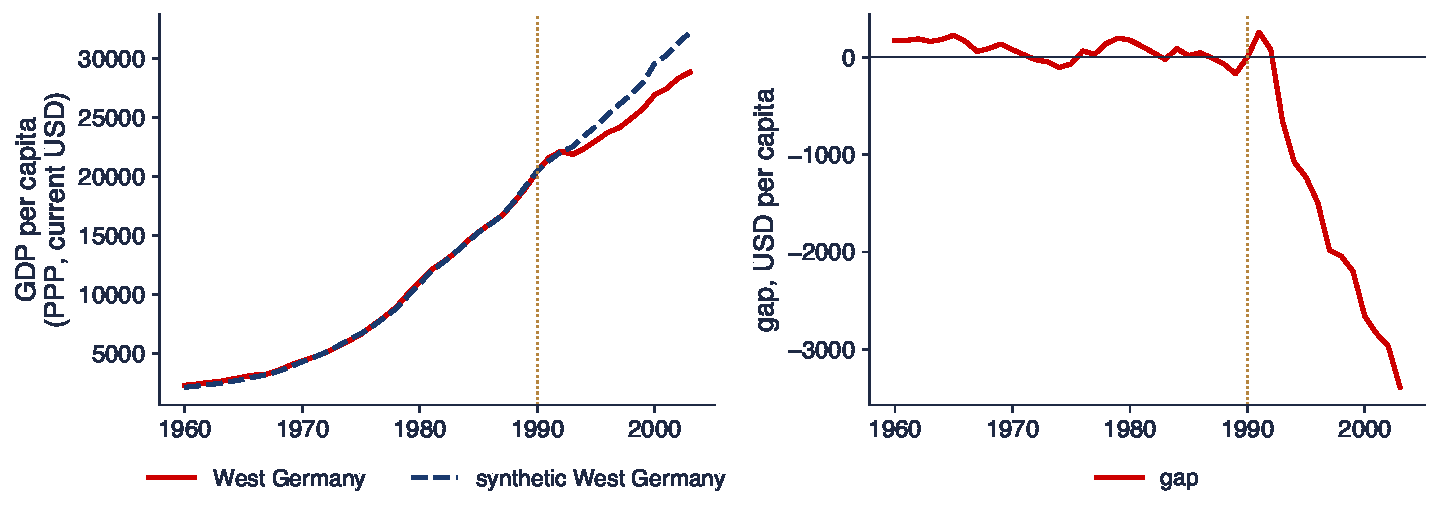
\includegraphics[width=0.97\textwidth,height=0.66\textheight,keepaspectratio]{ats_ch14_germany.pdf}
\end{center}
\vspace{-0.25cm}
\begin{itemize}
    \item Stînga: PIB pe locuitor (PPC, USD curenți); dreapta: diferența; RMSPE înainte de 1990: 121 USD
\end{itemize}
\quantlet{ATS\_ch14\_germany}{\qlurl{ATS_ch14_germany}}
\end{frame}

\begin{frame}{Interpretarea replicării germane}
\itemsize{\small}
\begin{itemize}
    \item Germania de Vest sintetică urmărește seria reală timp de treizeci de ani (1960--1989), apoi crește mai repede
    \item Diferența medie 1990--2003: $-$1588 USD pe locuitor pe an ($-$5{,}6\% din nivelul sintetic); în 2003: $-$3391 USD ($-$10{,}5\%)
    \item Lucrarea raportează o reducere de aproximativ 1600 USD pe an, în medie: replicarea coincide
    \item Donatorii (Austria, SUA, Japonia, Elveția, Țările de Jos) sînt economii bogate, industrializate: ponderile au sens economic, o verificare pe care niciun algoritm nu o face în locul nostru
\end{itemize}
\end{frame}

\begin{frame}{Testele placebo pentru cazul german}
\itemsize{\footnotesize}
\begin{center}
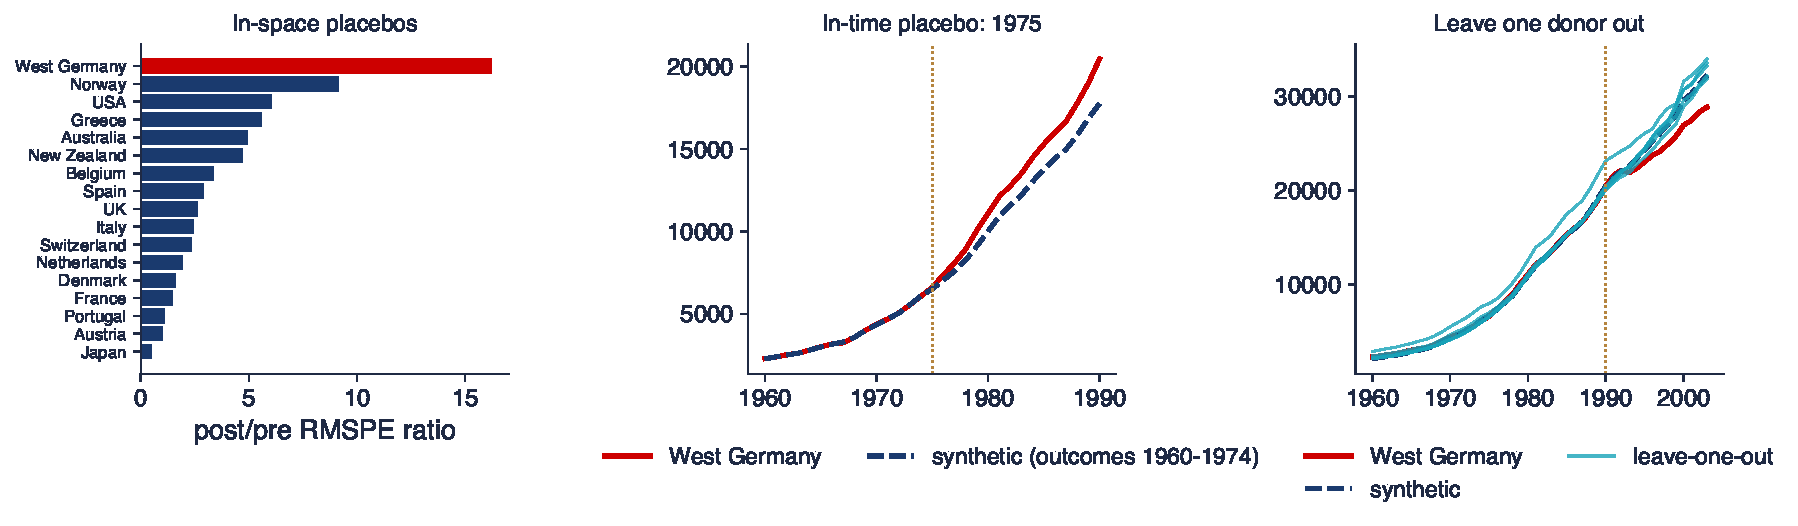
\includegraphics[width=0.97\textwidth,height=0.54\textheight,keepaspectratio]{ats_ch14_germany_placebo.pdf}
\end{center}
\vspace{-0.25cm}
\begin{itemize}
    \item Stînga: raportul RMSPE după/înainte de 1990 cînd fiecare țară este tratată pe rînd (ADH 2015, figura 6); centru: reunificarea mutată în 1975 (ca în figura 4, SC doar pe rezultat); dreapta: cîte un donator omis (figura 5)
\end{itemize}
\quantlet{ATS\_ch14\_germany}{\qlurl{ATS_ch14_germany}}
\end{frame}

\begin{frame}{Interpretarea testelor placebo germane}
\itemsize{\small}
\begin{itemize}
    \item Germania de Vest are cel mai mare raport (16{,}2; următoarea: Norvegia, 9{,}2): p-value-ul prin permutare $1/17$ = 0{,}059, cea mai mică posibilă
    \item Reunificare placebo în 1975 (SC doar pe rezultat, 1960--1974, RMSPE anterior 19 USD): Germania de Vest crește mai repede decît controlul sintetic (diferența medie +9{,}9\% pînă în 1990): nu apare niciun cost fals
    \item Cu predictorii publicați pentru 1975, $V$ ales prin validare încrucișată nu este identificat: un punct de pornire dă ca donator Austria, cel mai bun dintre opt dă Statele Unite \refKPSb
    \item Omiterea oricărui donator păstrează o diferență negativă în 2003, între 2965 și 5138 USD: rezultatul nu depinde de o singură țară
    \item Cu 17 unități, testul de permutare nu poate da $p < 0{,}059$
\end{itemize}
\end{frame}

\begin{frame}{Studiu de caz: dublura Brexit}
\itemsize{\small}
\begin{columns}[T]
\begin{column}{0.3\textwidth}
\centering

\includegraphics[height=0.32\textheight]{ch14_brexit_count_2016.jpg}\\[1mm]
\imgcap{Numărarea voturilor la referendumul privind UE, 23 iunie 2016}
\imgcredit{https://commons.wikimedia.org/wiki/File:At_the_Brexit_referendum_count_in_Borehamwood_(28176894300).jpg}{Foto: Steve Bowbrick (2016); CC BY 2.0; Wikimedia Commons}
\end{column}
\begin{column}{0.68\textwidth}
\begin{itemize}
    \item \refBMSS
    \begin{itemize}
        \item referendumul din 23 iunie 2016 ca experiment natural; rezultatul: PIB-ul real al Regatului Unit
    \end{itemize}
    \item Designul (secțiunea 2.1)
    \begin{itemize}
        \item 23 de donatori OCDE; PIB real trimestrial, normalizat la 1 în 1995
        \item perioada anterioară T1 1995 -- T2 2016; mediile a șase covariate
        \item ponderile publicate (tabelul 2): Statele Unite 0{,}51; Italia 0{,}17; Noua Zeelandă 0{,}14; Ungaria 0{,}11; Germania 0{,}05
    \end{itemize}
    \item Rezultatul publicat
    \begin{itemize}
        \item producția Regatului Unit cu 2,4\% sub dublură la sfîrșitul lui 2018
        \item semnificativ după testul de instabilitate la sfîrșitul eșantionului al lui \refAnd
    \end{itemize}
    \item Replicarea noastră
    \begin{itemize}
        \item aceiași donatori și aceeași fereastră; ediția curentă a datelor OCDE (pînă în T2 2026); doar traiectoria PIB (fără covariate)
    \end{itemize}
\end{itemize}
\end{column}
\end{columns}
\end{frame}

\begin{frame}{Dublura pe datele de azi}
\itemsize{\footnotesize}
\begin{center}
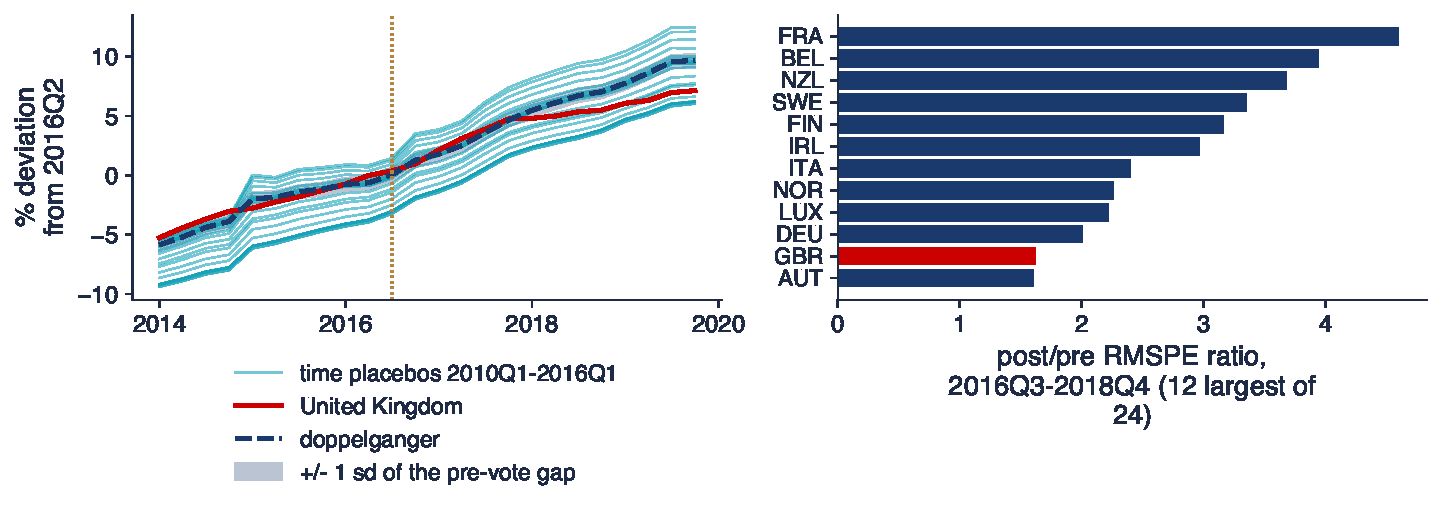
\includegraphics[width=0.97\textwidth,height=0.65\textheight,keepaspectratio]{ats_ch14_brexit.pdf}
\end{center}
\vspace{-0.25cm}
\begin{itemize}
    \item Stînga: PIB-ul real al Regatului Unit și dublura lui (\% față de T2 2016), cu dublurile voturilor fictive din fiecare trimestru T1 2010 -- T1 2016; dreapta: cele mai mari 12 rapoarte RMSPE după/înainte dintre cele 24 de țări
\end{itemize}
\quantlet{ATS\_ch14\_brexit}{\qlurl{ATS_ch14_brexit}}
\end{frame}

\begin{frame}{Interpretarea replicării Brexit}
\itemsize{\small}
\begin{itemize}
    \item Ponderile pe datele de azi: Statele Unite 0{,}36; Japonia 0{,}19; Canada 0{,}16; Portugalia 0{,}10; Ungaria 0{,}09; dublura se schimbă odată cu ediția datelor
    \item Diferența: 0{,}1\% în T4 2017, $-$1{,}5\% în T4 2018 (publicat: $-$2,4\%), $-$2{,}5\% în T4 2019; abaterea standard înainte de vot 0{,}51\%
    \item Regatul Unit este pe locul 11 din 24 în testele placebo pe țări; cele 25 de teste placebo în timp dau diferențe în T4 2018 între \ensuremath{-}4{,}3\% și 1{,}9\%: pe datele revizuite dovezile sînt mult mai slabe
    \item O replicare schimbă datele (revizuiri), specificația (fără covariate) și inferența (permutare în locul testului de la sfîrșitul eșantionului): raportați fiecare abatere separat
\end{itemize}
\end{frame}

\begin{frame}{Recapitulare: controlul sintetic}
\itemsize{\small}
\begin{itemize}
    \item O combinație convexă de donatori ajustată pe o perioadă lungă anterioară; justificată de un model factorial; ponderi rare și transparente
    \item Inferența prin placebo în spațiu și în timp, omiterea pe rînd a donatorilor, metode conformale; $p \ge 1/(J + 1)$
    \item Reunificarea Germaniei se replică exact; diferența Brexit este sensibilă la revizuirea datelor și la specificație
\end{itemize}
\end{frame}


%=============================================================================
\section{Dincolo de controlul sintetic}
%=============================================================================

\begin{frame}{Termenul liber și augmentarea}
\itemsize{\small}
\begin{itemize}
    \item \textbf{SC cu termen liber} \refDI, \refFP: permite o diferență constantă de nivel $c$ între unitatea tratată și donatori \[ \hat Y_{1t}(0) = c + \sum_j w_jY_{jt} \]
    \begin{itemize}
        \item ponderile se ajustează pe rezultatele anterioare minus media anterioară a fiecărei unități
        \item rezolvă partea de nivel a problemei înfășurătorii convexe; consistent cu potrivire imperfectă cînd factorii sînt staționari \refFP
    \end{itemize}
    \item \textbf{SC augmentat} \refASCM: corectează estimația SC cu dezechilibrul rămas al predictorilor, printr-o regresie ridge \[ \hat Y^{\mathrm{aug}}_{1t}(0) = \sum_j\hat w_jY_{jt} + \Big(X_1 - \sum_j\hat w_jX_j\Big)'\hat\eta_t \]
    \begin{itemize}
        \item $\hat w_j$: ponderile SC; $X_j$: rezultatele anterioare ale unității $j$; $\hat\eta_t$: coeficienții regresiei ridge a lui $Y_{jt}$ pe $X_j$, între donatori, cu penalizarea $\lambda$
        \item echivalent cu ponderile $\hat w + X_0(X_0'X_0 + \lambda I)^{-1}(X_1 - X_0'\hat w)$, care pot fi negative (extrapolare controlată)
        \item $\lambda \to \infty$ dă SC; $\lambda \to 0$ dă o regresie a rezultatului; deplasarea scade odată cu dezechilibrul rămas
    \end{itemize}
\end{itemize}
\end{frame}

\begin{frame}{Diferența în diferențe sintetică (1/2)}
\itemsize{\small}
\begin{itemize}
    \item \refSDID: o regresie cu efecte fixe pe unități și pe perioade, în care unitățile și perioadele sînt ponderate \[ (\hat\tau, \hat\mu, \hat\alpha, \hat\beta) = \arg\min\sum_{j,t}\big(Y_{jt} - \mu - \alpha_j - \beta_t - W_{jt}\tau\big)^2\hat\omega_j\hat\lambda_t \]
    \begin{itemize}
        \item $W_{jt} = 1$ pentru unitatea tratată după $T_0$, 0 altfel; $\tau$: efectul; $\mu$: media generală; $\alpha_j$: efectele fixe ale unităților; $\beta_t$: efectele fixe ale perioadelor
    \end{itemize}
    \item \textbf{Ponderile unităților} $\hat\omega_j$: SC cu termen liber și penalizare ridge
    \begin{itemize}
        \item penalizarea $\zeta^2T_0\|\omega\|^2$, cu $\zeta = (N_{\mathrm{tr}}T_{\mathrm{post}})^{1/4}\hat\sigma$; $N_{\mathrm{tr}}$: unitățile tratate; $T_{\mathrm{post}}$: perioadele de după; $\hat\sigma$: nivelul zgomotului controalelor
    \end{itemize}
    \item \textbf{Ponderile perioadelor} $\hat\lambda_t$: perioadele anterioare care prezic cel mai bine media controalelor după tratament
\end{itemize}
\end{frame}

\begin{frame}{Diferența în diferențe sintetică (2/2)}
\itemsize{\small}
\begin{itemize}
    \item Trei estimatori ca și cazuri particulare
    \begin{itemize}
        \item DiD: $\omega$ și $\lambda$ uniforme
        \item SC: doar ponderile unităților $\omega$ ($\lambda$ uniforme), fără efect fix al unității
        \item SDID: ambele seturi de ponderi, ambele efecte fixe
    \end{itemize}
    \item O singură unitate tratată: eroarea standard prin placebo
    \begin{itemize}
        \item fiecare control joacă pe rînd rolul unității tratate; abaterea standard a estimațiilor placebo este eroarea standard (algoritmul 4)
    \end{itemize}
\end{itemize}
\end{frame}

\begin{frame}{România 2025: designul controlului sintetic}
\itemsize{\small}
\begin{itemize}
    \item Rezultatul: inflația IAPC anuală (pp), $100(\ln P_t - \ln P_{t-12})$, Eurostat; unitatea tratată: România; donatori: celelalte 26 de țări UE
    \begin{itemize}
        \item $P_t$: indicele prețurilor IAPC în luna $t$; pp: puncte procentuale
        \item rata anuală elimină sezonalitatea și face vizibil un șoc al nivelului prețurilor exact douăsprezece luni
    \end{itemize}
    \item Perioada anterioară: iulie 2023 -- iunie 2025 (24 de luni, după valul 2021--2023); tratament din iulie 2025; fereastra efectului iulie 2025 -- iunie 2026
    \begin{itemize}
        \item o falsificare încorporată: după ce saltul nivelului prețurilor iese din fereastra de 12 luni (august 2026), diferența trebuie să dispară
    \end{itemize}
    \item Estimatori: SC, SC cu termen liber, SC augmentat ridge cu termen liber, SDID; inferența: placebo în spațiu
    \item Amenințări: măsurile proprii de energie și fiscale ale altor țări; anticiparea majorării TVA; România în afara domeniului donatorilor
\end{itemize}
\end{frame}

\begin{frame}{Patru contrafactuale pentru inflația României}
\itemsize{\footnotesize}
\begin{center}
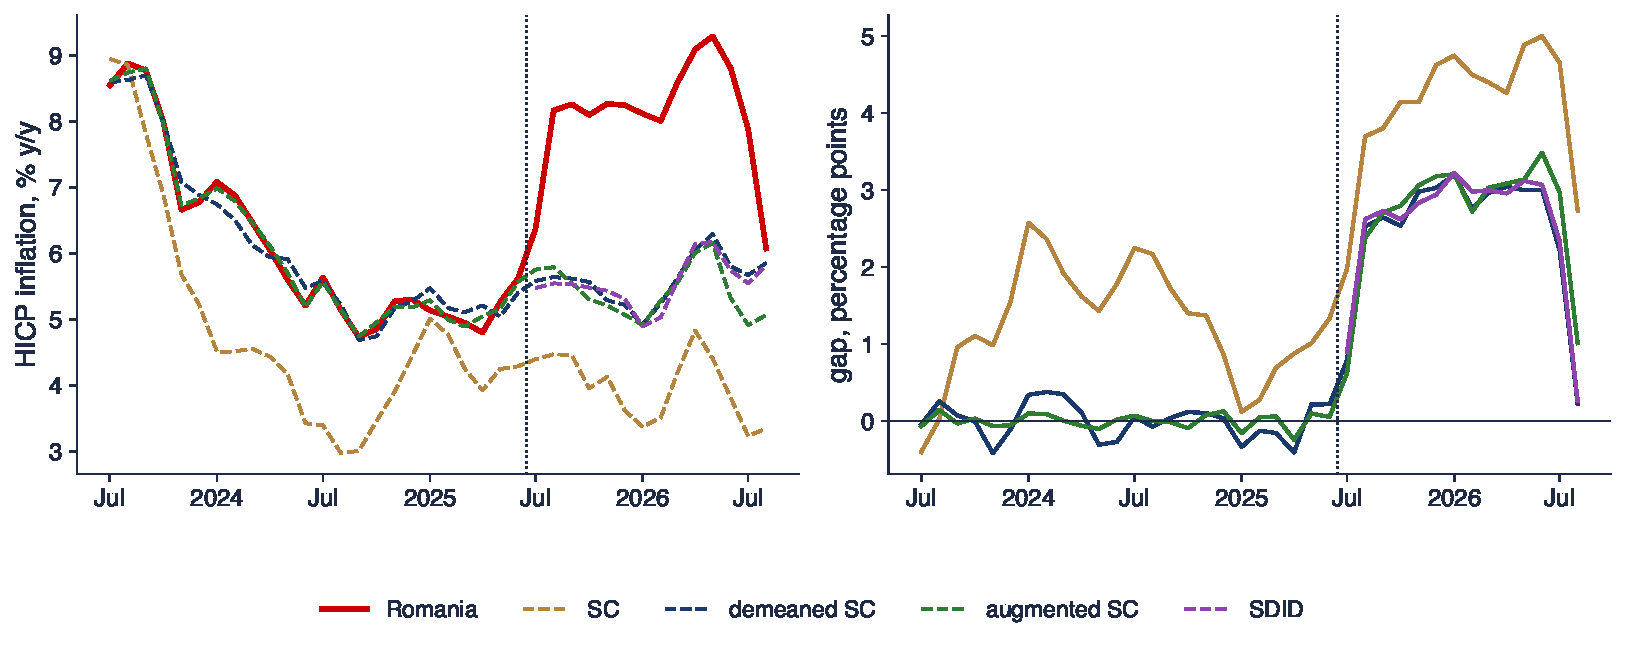
\includegraphics[width=0.97\textwidth,height=0.65\textheight,keepaspectratio]{ats_ch14_ro_sc.pdf}
\end{center}
\vspace{-0.25cm}
\begin{itemize}
    \item Stînga: România și cele patru contrafactuale estimate; dreapta: diferențele; linia verticală: iunie 2025; date pînă în august 2026
\end{itemize}
\quantlet{ATS\_ch14\_romania}{\qlurl{ATS_ch14_romania}}
\end{frame}

\begin{frame}{Interpretarea celor patru estimatori}
\itemsize{\small}
\begin{center}
\scriptsize
\begin{tabular}{lcccc}
\toprule
\textbf{Estimator} & \textbf{RMSPE anterior} & \textbf{august 2025} & \textbf{media iul. 2025 -- iun. 2026} & \textbf{august 2026} \\
\midrule
SC & 1{,}45 & 3{,}70 & 4{,}18 & 2{,}73 \\
SC cu termen liber & 0{,}23 & 2{,}53 & 2{,}70 & 0{,}22 \\
SC augmentat & 0{,}09 & 2{,}38 & 2{,}78 & 1{,}01 \\
SDID & -- & 2{,}62 & 2{,}75 ($se$ 0{,}70) & 0{,}26 \\
\bottomrule
\end{tabular}
\end{center}
\begin{itemize}
    \item SC clasic pune toată ponderea pe Croația 0{,}85; Ungaria 0{,}15: România se află în afara înfășurătorii convexe, potrivirea anterioară este slabă, iar efectul este supraestimat
    \item Cu termen liber potrivirea este bună (ponderi Franța 0{,}38; Slovenia 0{,}25; Suedia 0{,}13; Malta 0{,}10, ...); SC augmentat ($\lambda = 1$, 9 ponderi negative) și SDID sînt de acord: 2{,}7--2{,}8 pp pe douăsprezece luni
    \item Falsificarea: în august 2026 diferența scade la 0{,}22 (SC cu termen liber) și 0{,}26 (SDID); SC augmentat păstrează 1{,}01, prețul extrapolării cu ponderi negative
\end{itemize}
\end{frame}

\begin{frame}{Inferența prin placebo pentru România}
\itemsize{\footnotesize}
\begin{center}
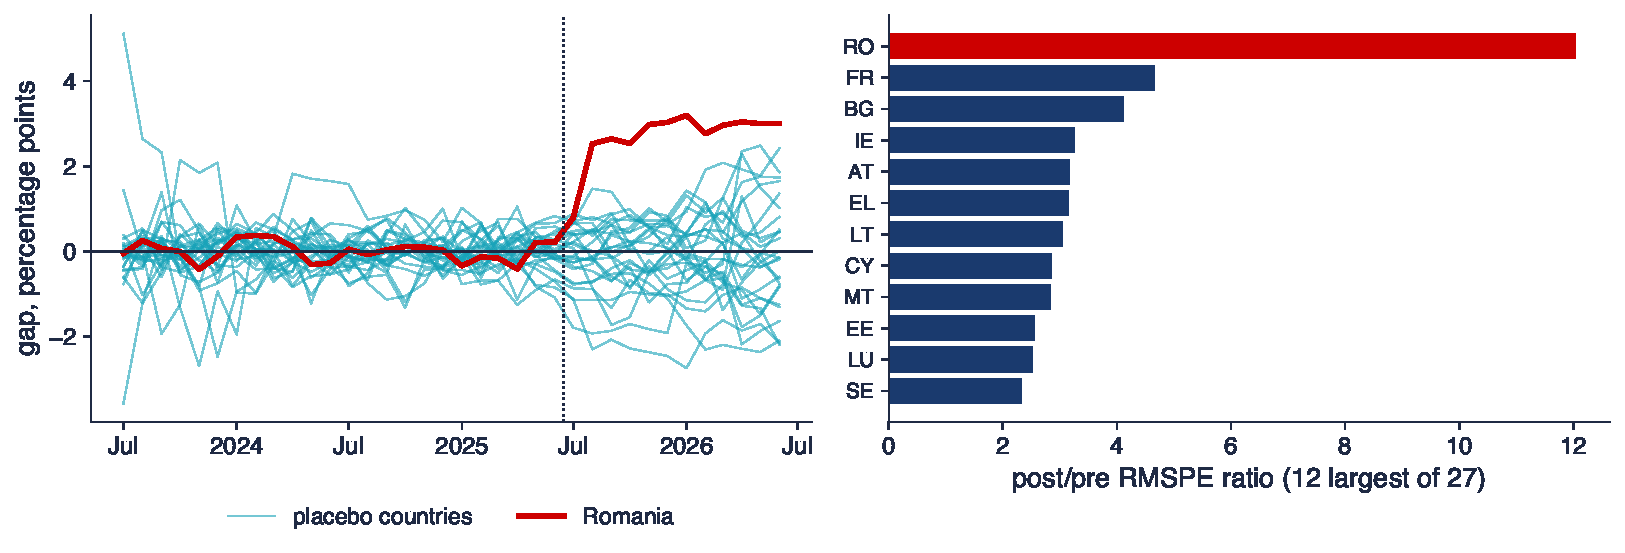
\includegraphics[width=0.97\textwidth,height=0.63\textheight,keepaspectratio]{ats_ch14_ro_placebo.pdf}
\end{center}
\vspace{-0.25cm}
\begin{itemize}
    \item SC cu termen liber aplicat pe rînd fiecărei țări UE; stînga: diferențele; dreapta: cele mai mari 12 rapoarte RMSPE după/înainte pe iulie 2025 -- iunie 2026
\end{itemize}
\quantlet{ATS\_ch14\_romania}{\qlurl{ATS_ch14_romania}}
\end{frame}

\begin{frame}{Interpretarea testelor placebo pentru România}
\itemsize{\small}
\begin{itemize}
    \item România are cel mai mare raport (12{,}0; următoarea Franța, 4{,}7): $p = 1/27$ = 0{,}037
    \item Nicio țară placebo nu are un salt de această mărime în iulie--august 2025: efectul nu este un șoc european comun
    \item P-value-ul prin permutare tratează România ca pe una dintre 27 de unități interschimbabile; este o măsură a rarității, nu o afirmație de încredere care decurge din eșantionare
    \item Măsurile altor țări din fereastră (schimbări fiscale, încheierea propriilor plafonări) deplasează efectul spre zero dacă au crescut inflația acolo
\end{itemize}
\end{frame}

\begin{frame}{Ponderea componentei fiscale}
\itemsize{\footnotesize}
\begin{center}
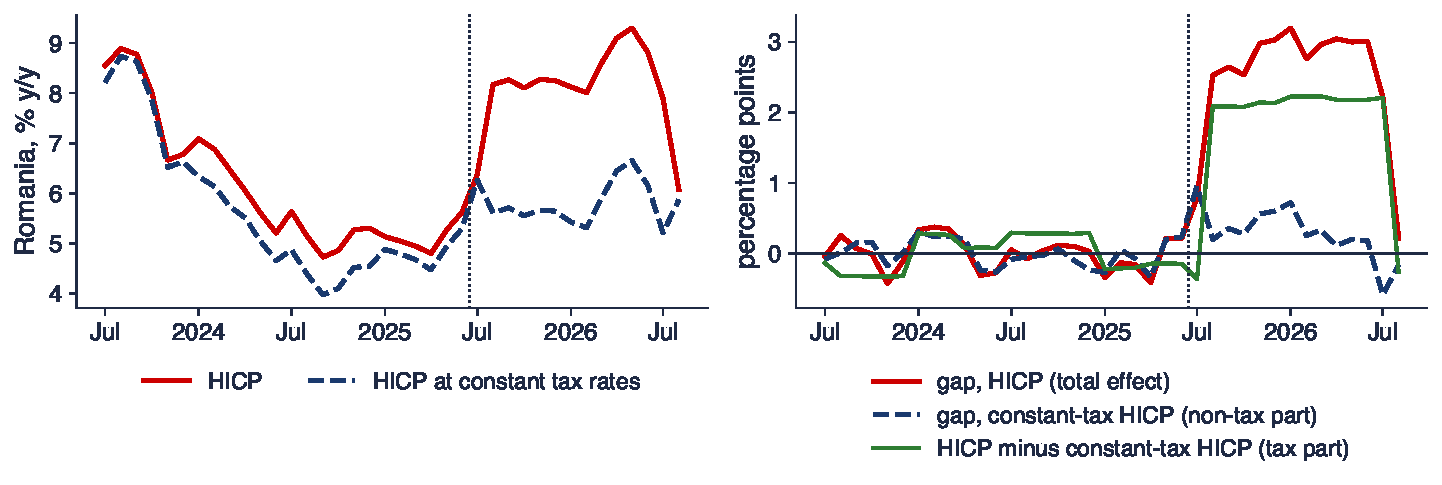
\includegraphics[width=0.97\textwidth,height=0.62\textheight,keepaspectratio]{ats_ch14_ro_tax.pdf}
\end{center}
\vspace{-0.25cm}
\begin{itemize}
    \item Stînga: IAPC al României și IAPC la cote de taxare constante (\refEuroCT); dreapta: diferența totală, diferența inflației la taxe constante (același SC cu termen liber pe toate țările) și componenta fiscală
\end{itemize}
\quantlet{ATS\_ch14\_romania}{\qlurl{ATS_ch14_romania}}
\end{frame}

\begin{frame}{Interpretarea descompunerii fiscale}
\itemsize{\small}
\begin{itemize}
    \item Indicele la taxe constante presupune transmiterea completă și imediată a modificărilor fiscale: componenta fiscală crește cu 2{,}09 pp în august 2025, cînd a crescut TVA
    \item Media pe douăsprezece luni: total 2{,}70 pp = componenta fiscală 1{,}95 pp + diferența la taxe constante 0{,}40 pp: aproximativ 72\% din efect este fiscal mecanic
    \item Partea nefiscală are maximul în iulie 2025 (0{,}96 pp): încheierea plafonării electricității, care este un preț, nu o taxă
    \item Transmiterea TVA în prețurile de consum este adesea incompletă și asimetrică \refBMKW; indicele la taxe constante este un reper contabil, nu o transmitere măsurată
\end{itemize}
\end{frame}

\begin{frame}{Adoptarea eșalonată și efectele fixe bidirecționale (1/2)}
\itemsize{\small}
\begin{itemize}
    \item Multe unități adoptă la date diferite $g$ (cohorta lor); regresia TWFE statică \[ Y_{it} = \alpha_i + \beta_t + \tau D_{it} + u_{it} \]
    \begin{itemize}
        \item $D_{it} = 1$ dacă unitatea $i$ este tratată la $t$; $\alpha_i$, $\beta_t$: efectele fixe ale unităților și ale perioadelor; $\tau$: un singur efect al tratamentului
    \end{itemize}
    \item \refGB: $\hat\tau$ este o medie ponderată a tuturor DiD 2$\times$2
    \begin{itemize}
        \item inclusiv a celor „interzise”, care folosesc unități deja tratate drept control
        \item cu efecte care cresc în timp, unele ponderi sînt negative \refdCDH: $\hat\tau$ poate avea chiar semnul greșit
    \end{itemize}
\end{itemize}
\end{frame}

\begin{frame}{Adoptarea eșalonată și efectele fixe bidirecționale (2/2)}
\itemsize{\small}
\begin{itemize}
    \item \refCSA: efecte pe grup și perioadă, fiecare comparat doar cu unitățile niciodată tratate \[ ATT(g, t) = \E[Y_t - Y_{g-1}\mid G = g] - \E[Y_t - Y_{g-1}\mid \text{niciodată tratat}] \]
    \begin{itemize}
        \item $G$: data de adoptare a unei unități; $Y_{g-1}$: rezultatul din ultima perioadă dinaintea adoptării; $ATT$: efectul mediu al tratamentului asupra unităților tratate
        \item apoi agregare după expunere ($t - g$) sau după cohortă
    \end{itemize}
    \item Metode înrudite: studii de eveniment ponderate prin interacțiuni \refSA; un ghid al noii literaturi DiD \refRSBP
    \item Testele trendurilor anterioare au putere mică; raportați sensibilitatea efectului la încălcarea trendurilor paralele
\end{itemize}
\end{frame}

\begin{frame}{TWFE față de Callaway și Sant'Anna}
\itemsize{\footnotesize}
\begin{center}
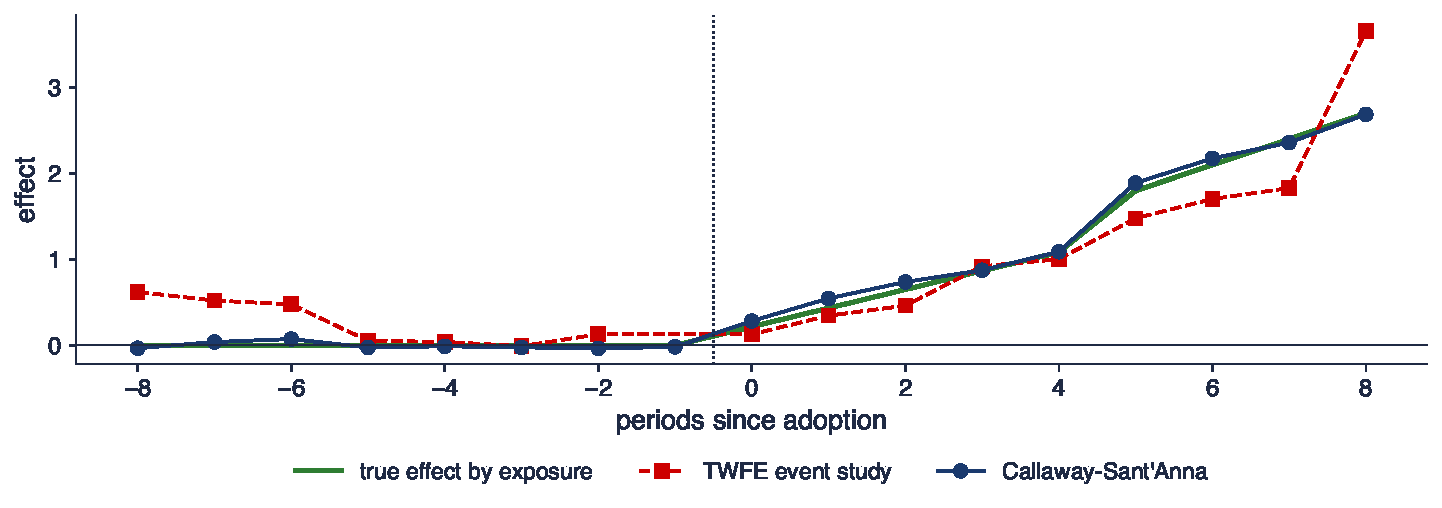
\includegraphics[width=0.97\textwidth,height=0.65\textheight,keepaspectratio]{ats_ch14_staggered.pdf}
\end{center}
\vspace{-0.25cm}
\begin{itemize}
    \item Panel simulat: trei cohorte care adoptă în perioadele 6, 11 și 16 și un grup niciodată tratat; efectele cresc cu expunerea, mai repede pentru cei care adoptă devreme
\end{itemize}
\quantlet{ATS\_ch14\_did\_dml}{\qlurl{ATS_ch14_did_dml}}
\end{frame}

\begin{frame}{Interpretarea adoptării eșalonate}
\itemsize{\small}
\begin{itemize}
    \item TWFE static: 0{,}55; efectul mediu real asupra tratatelor: 1{,}99; Callaway--Sant'Anna: 2{,}04
    \item TWFE folosește pe cei care adoptă devreme drept control pentru cei care adoptă tîrziu, în timp ce efectul lor încă crește: aceste comparații scad o parte din efect
    \item Studiul de eveniment TWFE este distorsionat la expuneri lungi (capătul grupat 3{,}66 față de 2{,}70); CS dă 2{,}69
    \item Cu o singură țară tratată (România) nu există eșalonare; cu politici la nivelul UE adoptate la date diferite, există
\end{itemize}
\end{frame}

\begin{frame}{Recapitulare: dincolo de controlul sintetic}
\itemsize{\small}
\begin{itemize}
    \item Termenul liber corectează diferențele de nivel; augmentarea ridge corectează dezechilibrul rămas; SDID combină ponderile unităților și ale perioadelor
    \item România 2025: 2{,}7--2{,}8 pp de inflație anuală în plus timp de douăsprezece luni, în mare parte efectul mecanic al TVA, și o falsificare confirmată
    \item Adoptarea eșalonată invalidează TWFE; folosiți estimatori pe grup și perioadă
\end{itemize}
\end{frame}


%=============================================================================
\section{Serii de timp structurale bayesiene și CausalImpact}
%=============================================================================

\begin{frame}{Modelul CausalImpact (1/2)}
\itemsize{\small}
\begin{itemize}
    \item \refCI: rezultatul este un trend plus o componentă sezonieră plus o regresie pe serii de control \[ y_t = \mu_t + \gamma_t + \beta'x_t + \varepsilon_t, \qquad \mu_{t+1} = \mu_t + \delta_t + \eta_t, \qquad \delta_{t+1} = \delta_t + \zeta_t \]
    \begin{itemize}
        \item $\mu_t$: nivelul local; $\delta_t$: panta locală; $\gamma_t$: componenta sezonieră; $x_t$: serii de control cu coeficienții $\beta$; $\varepsilon_t, \eta_t, \zeta_t$: zgomote independente cu distribuția Normală
    \end{itemize}
    \item Un model structural de serii de timp \refHar{} în formă de spațiu al stărilor, filtrat și netezit prin Kalman (\atschlink{https://danpele.github.io/Advanced-Time-Series/RO/Cursuri/capitol6_modele_spatiul_starilor_filtrare_bayesiana.pdf}{Capitolul 6}, \refDK)
    \begin{itemize}
        \item o distribuție a priori spike-and-slab pe $\beta$ selectează seriile de control \refSV; distribuția a posteriori se calculează prin MCMC
    \end{itemize}
\end{itemize}
\end{frame}

\begin{frame}{Modelul CausalImpact (2/2)}
\itemsize{\small}
\begin{itemize}
    \item Estimare pe perioada anterioară; se simulează contrafactualul de după $y^{(s)}_t(0)$ din distribuția predictivă a posteriori, dați $x_t$ observați
    \begin{itemize}
        \item $s$: indicele unei traiectorii simulate; efectele $y_t - y^{(s)}_t(0)$, punctuale și cumulate
        \item intervale de credibilitate din cuantilele efectelor simulate
    \end{itemize}
    \item \textbf{Identificarea}
    \begin{itemize}
        \item seriile de control \textbf{nu sînt afectate} de tratament
        \item relația lor cu $y$ rămîne stabilă după $T_0$
    \end{itemize}
\end{itemize}
\end{frame}

\begin{frame}{Implementarea folosită}
\itemsize{\small}
\begin{itemize}
    \item \texttt{statsmodels} \texttt{UnobservedComponents}: nivel local + regresie pe seriile de control, verosimilitate maximă pe perioada anterioară
    \begin{itemize}
        \item 1000 de traiectorii contrafactuale: parametrii extrași din distribuția lor normală asimptotică, apoi starea simulată înainte de la sfîrșitul perioadei anterioare, dați seriile de control observate
    \end{itemize}
    \item Diferențe față de pachetul R: fără selecție spike-and-slab, fără MCMC; incertitudinea parametrilor printr-o aproximare gaussiană
    \begin{itemize}
        \item versiunea transparentă păstrează fiecare pas vizibil; cu puține serii de control cele două dau intervale asemănătoare
    \end{itemize}
    \item Rezultate: efectul mediu cu un interval de 95\%, efectul cumulat și probabilitatea din coadă ca media contrafactuală să depășească media observată
\end{itemize}
\end{frame}

\begin{frame}{Studiu de caz: ETF-urile spot pe Bitcoin din SUA}
\itemsize{\small}
\begin{columns}[T]
\begin{column}{0.34\textwidth}
\centering
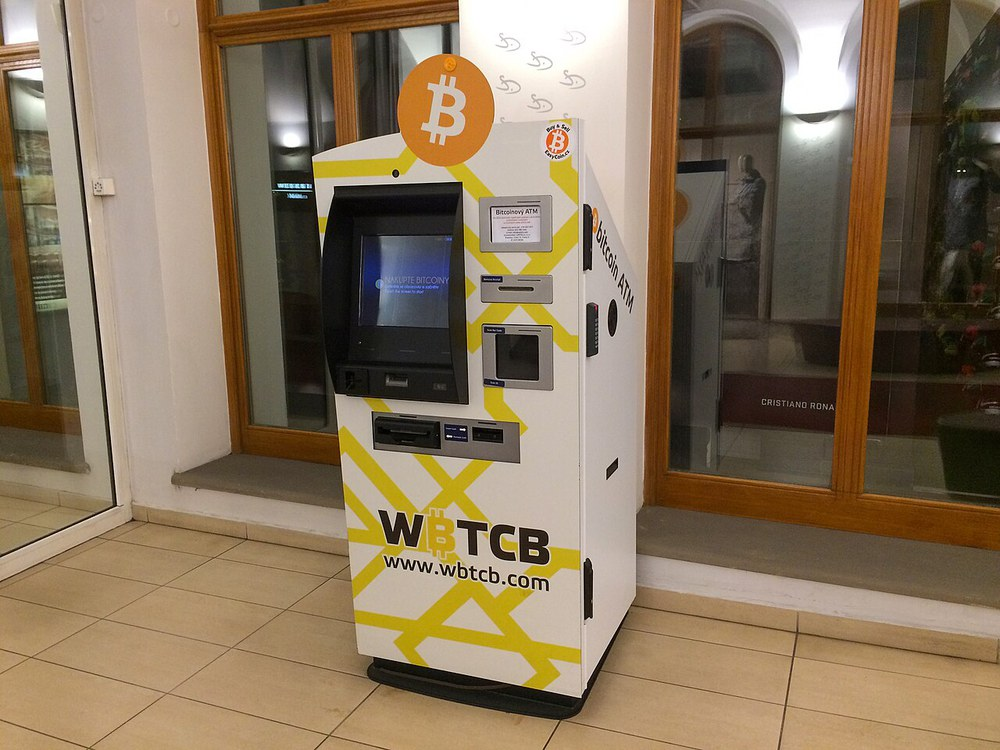
\includegraphics[height=0.40\textheight]{ch14_bitcoin_atm_2016.jpg}\\[1mm]
\imgcap{Un bancomat Bitcoin, Praga}
\imgcredit{https://commons.wikimedia.org/wiki/File:Bitcoin_ATM_Prague.jpg}{Foto: Perituss (2016); CC0; Wikimedia Commons}
\end{column}
\begin{column}{0.64\textwidth}
\begin{itemize}
    \item \textbf{10 ianuarie 2024} \refSEC
    \begin{itemize}
        \item SEC aprobă unsprezece ETP-uri (produse tranzacționate la bursă) spot pe Bitcoin; tranzacționarea începe pe 11 ianuarie
    \end{itemize}
    \item Întrebarea
    \begin{itemize}
        \item a schimbat aprobarea volatilitatea Bitcoin (cererea instituțională, arbitrajul între spot și ETF)?
    \end{itemize}
    \item Designul
    \begin{itemize}
        \item rezultatul: logaritmul varianței realizate săptămînale a Bitcoin
        \item serii de control: aceeași măsură pentru S\&P 500, Nasdaq 100, aur și EUR/USD
        \item perioada anterioară ianuarie 2023 -- 7 ianuarie 2024 (53 de săptămîni); după: 25 de săptămîni pînă în iunie 2024
    \end{itemize}
    \item Anticipare (liniile punctate)
    \begin{itemize}
        \item BlackRock a depus cererea pe 15 iunie 2023; o instanță a decis în favoarea Grayscale pe 29 august 2023
    \end{itemize}
\end{itemize}
\end{column}
\end{columns}
\end{frame}

\begin{frame}{CausalImpact pentru aprobarea ETF-urilor spot}
\itemsize{\footnotesize}
\begin{center}
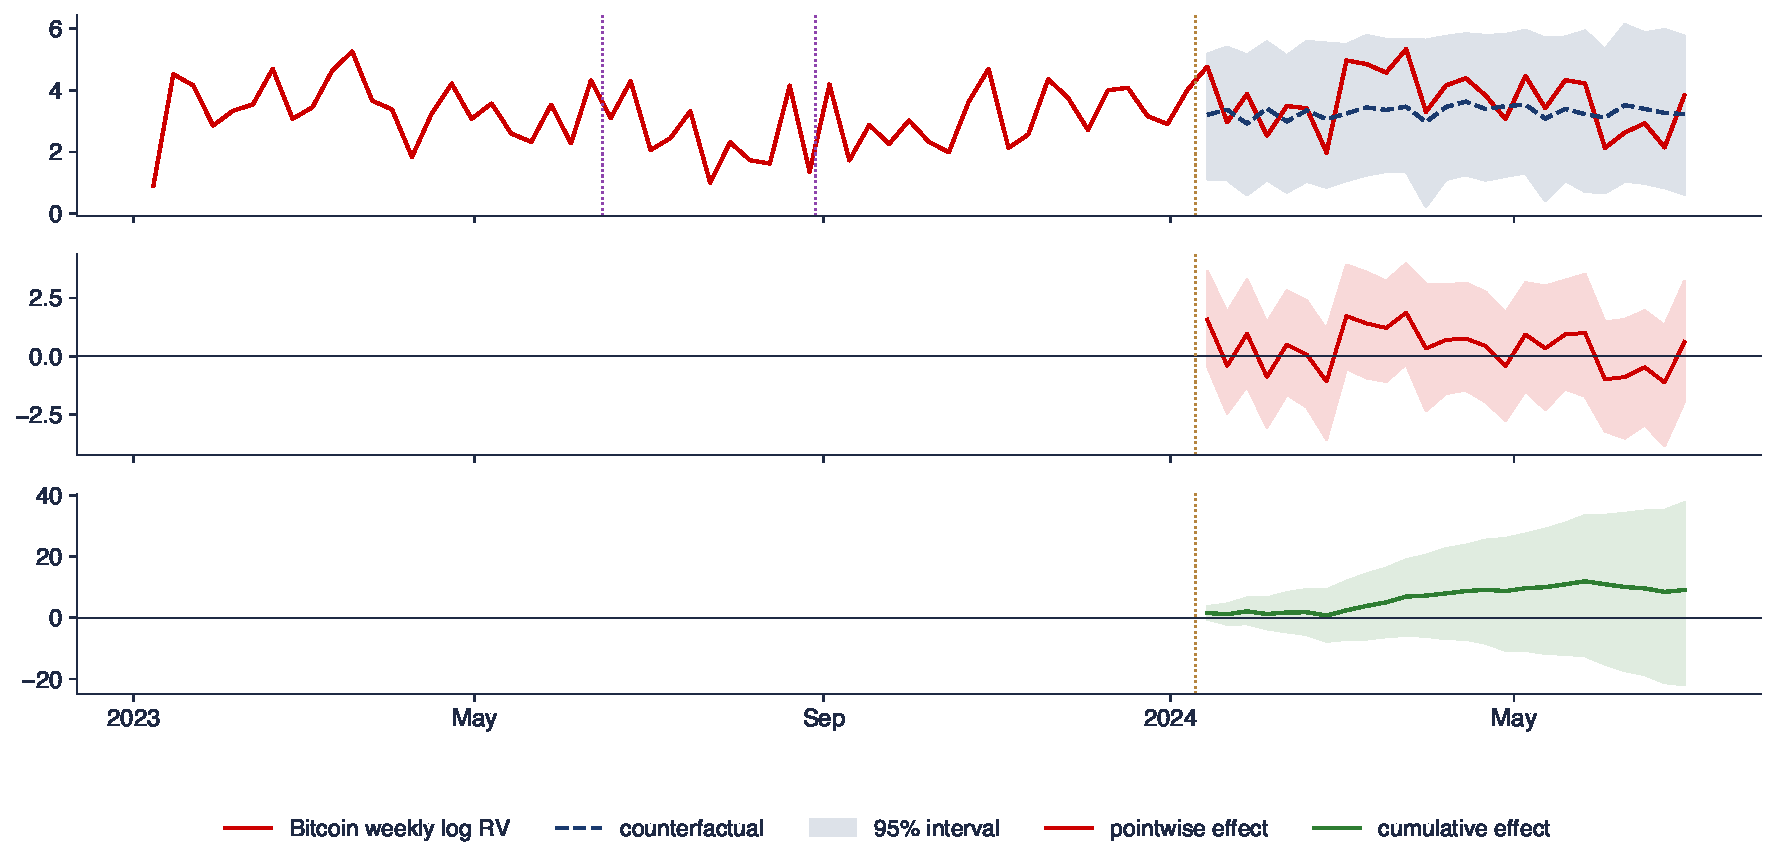
\includegraphics[width=0.97\textwidth,height=0.68\textheight,keepaspectratio]{ats_ch14_btc.pdf}
\end{center}
\vspace{-0.25cm}
\begin{itemize}
    \item Sus: log RV observat și contrafactual, cu interval de 95\%; mijloc: efectul punctual; jos: efectul cumulat
\end{itemize}
\quantlet{ATS\_ch14\_causalimpact}{\qlurl{ATS_ch14_causalimpact}}
\end{frame}

\begin{frame}{Interpretarea analizei ETF}
\itemsize{\small}
\begin{itemize}
    \item Efectul mediu asupra log RV săptămînal: 0{,}36 (interval de 95\% [\ensuremath{-}0{,}87; 1{,}50]), probabilitatea din coadă 0{,}26: nicio schimbare detectabilă
    \item Varianța nivelului este mică (0{,}011) față de cea neregulată (0{,}94): volatilitatea cripto săptămînală este în mare parte zgomot, iar seriile de control explică puțin
    \item Rezultatul este în acord cu un studiu publicat: niciun efect asupra volatilității proprii a Bitcoin \refBBG
    \item Lipsa dovezilor nu este dovada lipsei: cu acest zgomot, o modificare de 50\% a volatilității nu ar fi detectată
\end{itemize}
\end{frame}

\begin{frame}{Date placebo și alegerea seriilor de control}
\itemsize{\footnotesize}
\begin{center}
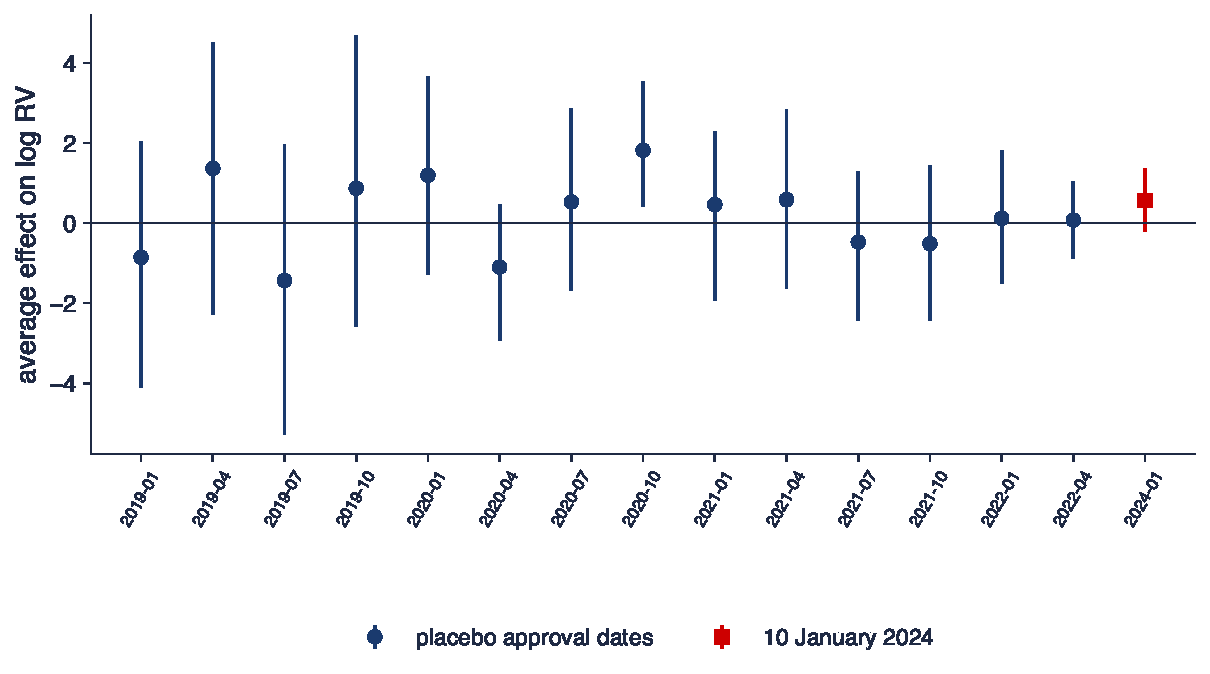
\includegraphics[width=0.97\textwidth,height=0.65\textheight,keepaspectratio]{ats_ch14_btc_placebo.pdf}
\end{center}
\vspace{-0.25cm}
\begin{itemize}
    \item Aceeași analiză cu 14 date fictive de aprobare în 2019--2022 (cîte 53 de săptămîni înainte și 25 după) și data reală cu aceleași lungimi ale ferestrelor
\end{itemize}
\quantlet{ATS\_ch14\_causalimpact}{\qlurl{ATS_ch14_causalimpact}}
\end{frame}

\begin{frame}{Interpretarea datelor placebo}
\itemsize{\small}
\begin{itemize}
    \item Doar 1 dintre cele 14 intervale placebo exclude zero; estimațiile placebo au abaterea standard 0{,}97: estimația reală se află în domeniul lor
    \item Cu Ether ca serie de control suplimentară: 0{,}18 [\ensuremath{-}0{,}47; 0{,}87]; dar Ether poate răspunde el însuși la aprobare: un control tratat deplasează efectul spre zero
    \item Mutarea lui $T_0$ la depunerea cererii BlackRock (iunie 2023): \ensuremath{-}0{,}02 [\ensuremath{-}1{,}74; 1{,}62]: tot nimic, deci anticiparea nu ascunde un efect mare
    \item Datele placebo calibrează intervalele de credibilitate: dacă multe teste placebo par „semnificative”, modelul este greșit specificat
\end{itemize}
\end{frame}

\begin{frame}{Recapitulare: BSTS și CausalImpact}
\itemsize{\small}
\begin{itemize}
    \item O prognoză în spațiul stărilor a traiectoriei netratate pe baza seriilor de control; incertitudinea vine din parametri și din stări
    \item Ipoteza esențială privește seriile de control: neafectate și într-o relație stabilă; verificați cu date placebo
    \item Aprobarea ETF-urilor spot nu a schimbat detectabil volatilitatea Bitcoin; designul nu ar fi putut vedea efecte mici
\end{itemize}
\end{frame}


%=============================================================================
\section{Double machine learning și identificarea onestă}
%=============================================================================

\begin{frame}{Double/debiased machine learning pentru serii de timp (1/2)}
\itemsize{\small}
\begin{itemize}
    \item \refDML: \textbf{modelul parțial liniar} \[ y_t = \theta d_t + g(X_t) + u_t, \qquad d_t = m(X_t) + v_t \]
    \begin{itemize}
        \item $d_t$: tratamentul; $\theta$: efectul lui; $X_t$: variabilele de control; $g$, $m$: \textbf{funcții auxiliare} necunoscute, învățate prin machine learning; $u_t, v_t$: erori
    \end{itemize}
    \item \textbf{Scorul ortogonal}: se regresează reziduul lui $y$ pe reziduul lui $d$ \[ \psi = \big(y_t - \ell(X_t) - \theta(d_t - m(X_t))\big)\big(d_t - m(X_t)\big), \qquad \ell(X) = \E[y\mid X] \]
    \begin{itemize}
        \item $\hat\theta$ rezolvă $\frac1T\sum_t\psi_t = 0$; insensibil de ordinul întîi la erorile din $\ell$ și $m$
    \end{itemize}
\end{itemize}
\end{frame}

\begin{frame}{Double/debiased machine learning pentru serii de timp (2/2)}
\itemsize{\small}
\begin{itemize}
    \item \textbf{Cross-fitting}: funcțiile auxiliare sînt estimate pe alte subeșantioane decît cel pe care se evaluează $\psi$
    \begin{itemize}
        \item pentru serii de timp se folosesc \textbf{blocuri contigue}, cu un interval de separare în jurul blocului omis
        \item eroarea standard dintr-o varianță HAC a lui $\psi$
    \end{itemize}
    \item DML elimină deplasarea din regularizare și supraajustare; nu creează identificare
    \begin{itemize}
        \item $d_t$ trebuie să fie neconfundat, dat $X_t$
    \end{itemize}
\end{itemize}
\end{frame}

\begin{frame}{DML față de o ajustare liniară}
\itemsize{\footnotesize}
\begin{center}
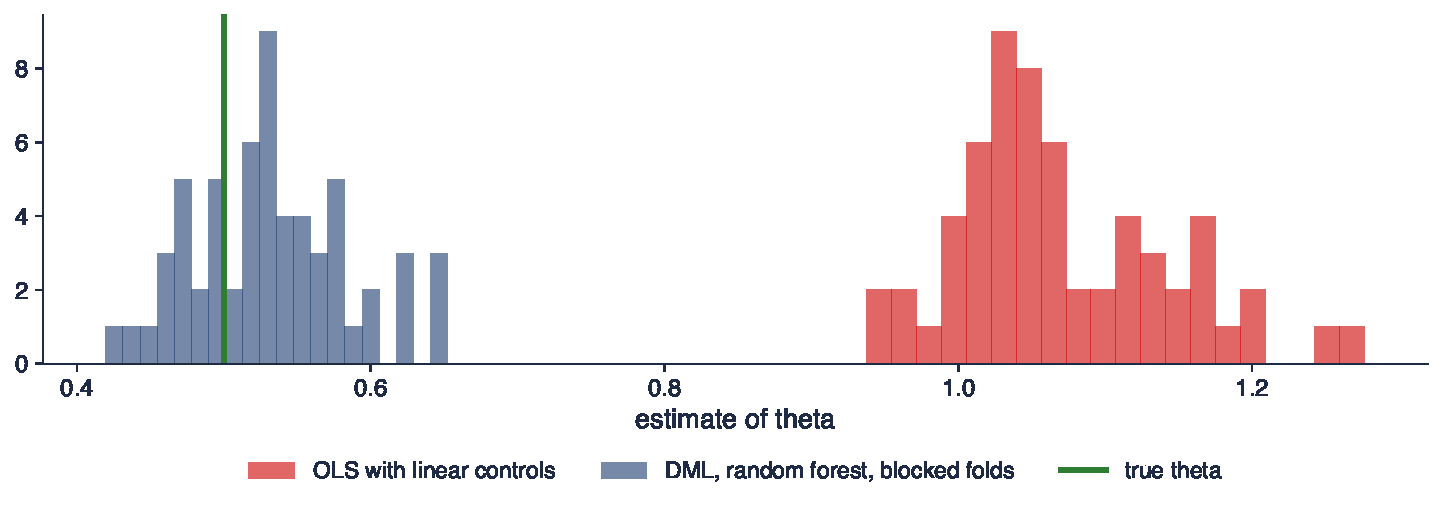
\includegraphics[width=0.97\textwidth,height=0.65\textheight,keepaspectratio]{ats_ch14_dml.pdf}
\end{center}
\vspace{-0.25cm}
\begin{itemize}
    \item Date dependente simulate: 10 covariate VAR(1), $g$ și $m$ neliniare, erori AR(1), $\theta = 0{,}5$, $T = 1\,000$, 60 de repetări; păduri aleatoare cu cinci blocuri
\end{itemize}
\quantlet{ATS\_ch14\_did\_dml}{\qlurl{ATS_ch14_did_dml}}
\end{frame}

\begin{frame}{Interpretarea experimentului DML}
\itemsize{\small}
\begin{itemize}
    \item OLS cu controale liniare: estimația medie 1{,}07, departe de 0,5: confuzia neliniară nu este eliminată
    \item DML: media 0{,}53, abaterea standard 0{,}05; intervalele HAC de 95\% acoperă valoarea reală în 88\% din repetări
    \item Deplasarea rămasă provine din erorile pădurilor pe un eșantion finit; scade cînd $T$ crește
    \item În seriile de timp macro, tratamentul este rar neconfundat, dați factorii observați: DML este un instrument pentru etapa de estimare, după ce identificarea a fost argumentată
\end{itemize}
\end{frame}

\begin{frame}{Identificarea, metodă cu metodă}
\itemsize{\small}
\begin{center}
\scriptsize
\begin{tabular}{>{\raggedright\arraybackslash}p{2.6cm}>{\raggedright\arraybackslash}p{5.4cm}>{\raggedright\arraybackslash}p{4.4cm}}
\toprule
\textbf{Metoda} & \textbf{Ipoteza esențială} & \textbf{Verificarea} \\
\midrule
Granger, PCMCI & nicio cauză comună ascunsă; momentul observării corect; fidelitate & adăugați posibili factori de confuzie; schimbați frecvența \\
ITS, studiu de eveniment & nimic altceva nu se schimbă la $T_0$; nicio anticipare & date placebo; cronologia știrilor \\
Control sintetic, SDID & model factorial; donatori neafectați; unitatea tratată în domeniul donatorilor & potrivirea anterioară, placebo, omiterea pe rînd \\
DiD (eșalonat) & trenduri paralele; nicio anticipare & trenduri anterioare cu analiză de sensibilitate \\
CausalImpact & controale neafectate; relație stabilă & date placebo; alte seturi de controale \\
SVAR, LP, DML & la fel de bun ca aleator, dat trecutul sau un instrument & dovezi narative; puterea instrumentului \\
\bottomrule
\end{tabular}
\end{center}
\end{frame}

\begin{frame}{Raportarea onestă}
\itemsize{\small}
\begin{itemize}
    \item Precizați mărimea țintă (ce efect, asupra cărei unități, pe ce orizont) înainte de a alege metoda
    \item Fixați datele tratamentului, ferestrele, donatorii și estimatorii înainte de a privi datele de după tratament; publicați preînregistrarea
    \item Raportați fiecare placebo, fiecare specificație și fiecare abatere de la designul publicat; o curbă a specificațiilor le arată împreună
    \item Separați incertitudinea statistică (intervalele) de incertitudinea identificării (ipotezele); a doua este de obicei mai mare
    \item Citiți \refAI{} și \refAba{} înainte de a scrie o evaluare de politică
\end{itemize}
\end{frame}


%=============================================================================
\section{AI în descoperirea științifică}
%=============================================================================

\begin{frame}{O întrebare deschisă}
\itemsize{\small}
\begin{itemize}
    \item Întrebarea
    \begin{itemize}
        \item cît din creșterea inflației din România în 2025--2026 a fost cauzată de încheierea plafonării electricității și de majorarea TVA?
        \item cît de robust este răspunsul la alegerea metodei?
    \end{itemize}
    \item O formă testabilă
    \begin{itemize}
        \item formal: $H_0$: diferența medie pe iulie 2025 -- iunie 2026 este zero; afirmația „între 2 și 3,5 pp” trebuie să fie valabilă pentru orice estimator preînregistrat cu potrivire anterioară bună
        \item infirmată dacă o specificație rezonabilă dă mai puțin de 2 pp sau dacă o țară placebo egalează România
    \end{itemize}
    \item Miza
    \begin{itemize}
        \item politica monetară trebuie să distingă efectele unice asupra nivelului prețurilor de inflația persistentă
        \item efectele de runda a doua determină deciziile privind dobînzile
        \item literatura de pornire: \refADHb, \refASCM, \refSDID, \refBMKW
    \end{itemize}
\end{itemize}
\end{frame}

\begin{frame}{Bucla de cercetare cu un asistent AI}
\itemsize{\footnotesize}
\begin{itemize}
    \item Un asistent AI (un LLM precum Claude, ChatGPT, Gemini sau Copilot) accelerează fiecare etapă; Semantic Scholar și Elicit ajută la literatură
    \begin{itemize}
        \item \textbf{literatura}: \aiprompt{Listează studii recenzate din 2015 încoace care estimează transmiterea TVA în prețurile de consum cu control sintetic sau DiD; dă DOI-urile și transmiterea estimată.} Apoi verificați fiecare DOI pe Crossref
        \item \textbf{designul}: \aiprompt{Scrie o preînregistrare: rezultatul, donatorii, excluderile, perioada anterioară, estimatorii, testele placebo, ce înseamnă un efect robust.}
        \item \textbf{cod și replicare}: reproduceți întîi ponderile germane (Austria 0{,}42; SUA 0{,}22; ...) înainte de a rula ceva pe România
        \item \textbf{critica}: \aiprompt{Joacă rolul unui recenzent ostil: ce țări UE au avut propriile măsuri de energie sau fiscale în 2025--2026 și cum ar deplasa fiecare estimația?}
    \end{itemize}
    \item Raportul: ce s-a cerut, ce s-a păstrat, ce s-a respins (AI\_USE.md, AI\_ERRORS.md)
\end{itemize}
\end{frame}

\begin{frame}{Verificări necesare}
\itemsize{\small}
\begin{itemize}
    \item Fiecare referință există și spune ce se afirmă (DOI-ul funcționează, titlul coincide, rezultatul se află în lucrare)
    \item Datele politicilor se iau din surse oficiale (Monitorul Oficial, Eurostat, SEC), nu din memoria asistentului
    \item Grupul donatorilor exclude țările cu propriile șocuri mari în fereastră, iar excluderile sînt scrise înainte de a vedea rezultatele
    \item Testele placebo sînt rulate cu exact același cod și aceleași setări ca estimația principală
    \item O afirmație AI de tipul „controlul sintetic dovedește că TVA a cauzat 3 pp de inflație” se reformulează ca o estimație cu ipoteze
\end{itemize}
\end{frame}

\begin{frame}{Mini studiu de caz: curba specificațiilor pentru România}
\itemsize{\footnotesize}
\begin{center}
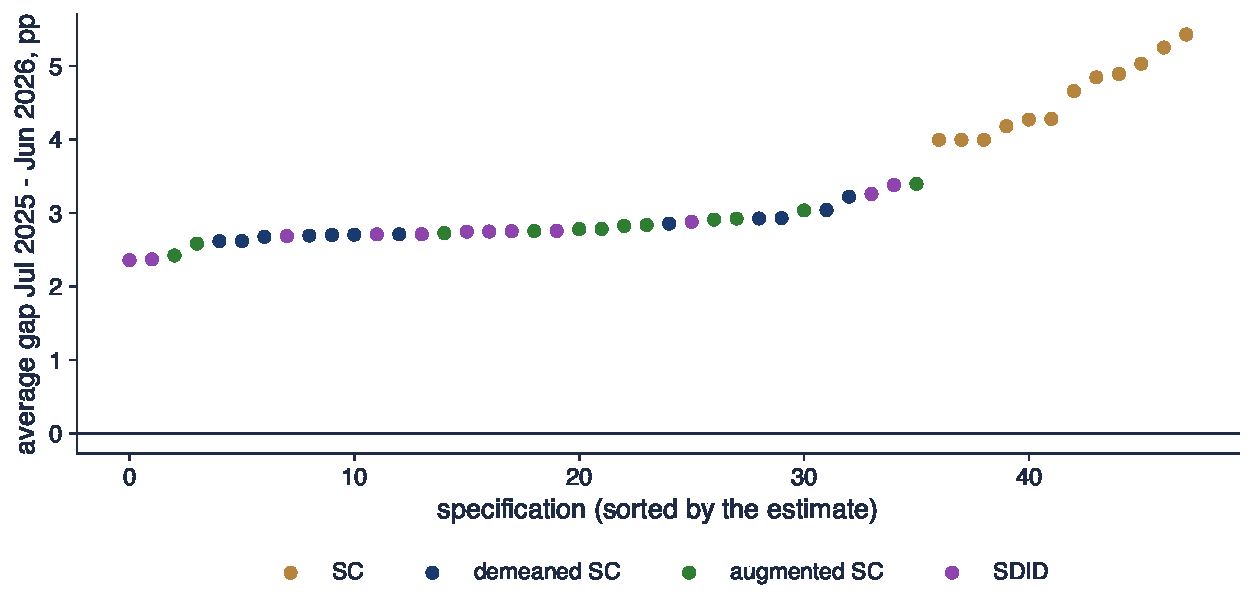
\includegraphics[width=0.97\textwidth,height=0.56\textheight,keepaspectratio]{ats_ch14_ai_case.pdf}
\end{center}
\vspace{-0.25cm}
\begin{itemize}
    \item 48 de specificații: patru estimatori $\times$ trei grupuri de donatori (UE-26, zona euro, UE din afara zonei euro) $\times$ patru perioade anterioare (din 2017, 2019, iulie 2023, 2024; valul 2021--2023 exclus)
    \item Fără SC clasic: între 2{,}36 și 3{,}40 pp, mediana 2{,}75; SC clasic: mediana 4{,}47 (potrivire anterioară slabă); 0 specificații dau un efect nepozitiv: ipoteza rezistă
\end{itemize}
\quantlet{ATS\_ch14\_ai\_case}{\qlurl{ATS_ch14_ai_case}}
\end{frame}

\begin{frame}{Idee de proiect}
\itemsize{\small}
\begin{itemize}
    \item \textbf{Transmiterea taxelor în Europa Centrală și de Est cu controale sintetice}: întîi replicare, apoi extindere
    \begin{itemize}
        \item replicați: \refADHb{} (tabelul 1, figurile 2--5) cu datele publice, apoi estimația pentru România din acest capitol
        \item extindeți: IAPC pe grupe de produse (alimente, energie, servicii) pentru a măsura transmiterea pe cote de TVA
        \item alte episoade (Ungaria 2012, adoptarea euro în Croația în 2023); intervale conformale \refCWZ
        \item preînregistrați: donatorii și excluderile, ferestrele, estimatorii, testele placebo, regula de robustețe
    \end{itemize}
    \item Livrabilele urmează regulile cursului: repository, raport, AI\_USE.md, AI\_ERRORS.md, susținere orală
\end{itemize}
\end{frame}


%=============================================================================
\section{Încheiere}
%=============================================================================

\begin{frame}{Idei de reținut}
\itemsize{\small}
\begin{itemize}
    \item Cauzalitatea Granger și metodele înrudite (TE, PCMCI, CCM) descriu structura predictivă; afirmațiile cauzale cer ipoteze despre alocarea tratamentului
    \item Seriile întrerupte și studiile de eveniment folosesc propriul trecut al unității; dependența le mărește erorile standard
    \item Controlul sintetic și succesorii lui folosesc alte unități; testele placebo sînt inferența, potrivirea pe o perioadă lungă este justificarea
    \item Replicarea arată fragilitatea: rezultatul reunificării Germaniei se menține, diferența Brexit depinde de ediția datelor
    \item România 2025: un efect robust de 2{,}7--2{,}8 pp pe douăsprezece luni, în mare parte TVA mecanic; ETF-urile Bitcoin: niciun efect detectabil asupra volatilității
\end{itemize}
\end{frame}

\begin{frame}{Autoevaluare}
\itemsize{\small}
\begin{columns}[T]
\begin{column}{0.58\textwidth}
\begin{block}{Întrebări}
\begin{itemize}
    \item De ce poate adăugarea unei variabile la mulțimea de informație să elimine o cauzalitate Granger?
    \item Ce obține condiționarea pe părinții sursei în testul MCI?
    \item De ce eșuează controlul sintetic clasic pentru inflația României?
    \item Care este cel mai mic p-value placebo cu 23 de donatori?
    \item De ce poate o estimație TWFE statică să aibă semnul greșit în cazul adoptării eșalonate?
\end{itemize}
\end{block}
\end{column}
\begin{column}{0.38\textwidth}
\begin{block}{Urmează: \atschlink{https://danpele.github.io/Advanced-Time-Series/RO/Cursuri/capitol15_recapitulare_proiecte.pdf}{Capitolul 15}}
\begin{itemize}
    \item Recapitulare și susținerea proiectelor
    \item o sinteză pentru fiecare capitol; proiectul de replicare și susținerea orală
\end{itemize}
\end{block}
\end{column}
\end{columns}
\end{frame}


%=============================================================================
\section{Anexă}
%=============================================================================

\begin{frame}{Anexă: marginea deplasării controlului sintetic}
\hypertarget{atsapp1}{}\atsappback{atssrc2}{Înapoi}
\itemsize{\small}
\begin{itemize}
    \item Modelul factorial $Y_{jt}(0) = \delta_t + \lambda_t\mu_j + \varepsilon_{jt}$ ($F$ factori); ponderi cu $\sum_jw_jY_{jt} = Y_{1t}$, $t \le T_0$
    \item Stivuim perioada anterioară: $\lambda^P(\mu_1 - \sum_jw_j\mu_j) = -(\varepsilon^P_1 - \sum_jw_j\varepsilon^P_j)$; dacă $\lambda^{P\prime}\lambda^P$ este inversabilă, obținem dezechilibrul încărcărilor
    \item Atunci $Y_{1t}(0) - \sum_jw_jY_{jt} = \lambda_t(\lambda^{P\prime}\lambda^P)^{-1}\lambda^{P\prime}\sum_jw_j\varepsilon^P_j - \dots + (\varepsilon_{1t} - \sum_jw_j\varepsilon_{jt})$
    \item Primul termen are media zero doar aproximativ (ponderile depind de $\varepsilon^P$); ADH (2010, anexa B) îl mărginesc printr-o mărime de ordinul $J^{1/p}\bar m_p^{1/p}F\,\bar\lambda^2/(\xi T_0^{1 - 1/p})$: mică atunci cînd $T_0$ este mare relativ la $J$
\end{itemize}
\end{frame}

\begin{frame}{Anexă: entropia de transfer gaussiană este jumătate din măsura Geweke}
\hypertarget{atsapp2}{}\atsappback{atssrc1}{Înapoi}
\itemsize{\small}
\begin{itemize}
    \item Pentru variabile gaussiene comune, $I(Y; X\mid Z) = \frac12\ln\dfrac{\mathrm{Var}(Y\mid Z)}{\mathrm{Var}(Y\mid X, Z)}$ (entropia unei variabile gaussiene este $\frac12\ln(2\pi e\sigma^2)$)
    \item Cu $Y = y_t$, $X = x^{(l)}_{t-1}$, $Z = y^{(k)}_{t-1}$, varianțele condiționate sînt varianțele reziduale ale regresiilor Granger restrînsă și completă
    \item Deci $TE_{x\to y} = \frac12F_{x\to y}$, iar $2T\cdot\widehat{TE} \approx T\hat F \approx W$, forma de raport de verosimilitate a testului Wald Granger \refBBS
    \item Datele negaussiene anulează egalitatea: TE detectează atunci dependențe pe care un test liniar le ratează (secțiunea 1)
\end{itemize}
\end{frame}


%=============================================================================
\section{Bibliografie}
%=============================================================================

\begin{frame}{Bibliografie (1/5)}
\itemsize{\tiny}
\begin{itemize}
    \item Abadie, A., Diamond, A., \& Hainmueller, J. (2015). Comparative politics and the synthetic control method. \textit{American Journal of Political Science}, 59(2), 495--510. \href{https://doi.org/10.1111/ajps.12116}{doi:10.1111/ajps.12116}
    \item Abadie, A., Diamond, A., \& Hainmueller, J. (2014). Replication data for: Comparative politics and the synthetic control method. Harvard Dataverse, version 2.1 (CC0); erratum and updated archive, version 3 (2026). \href{https://doi.org/10.7910/DVN/24714}{doi:10.7910/DVN/24714}
    \item Abadie, A., Diamond, A., \& Hainmueller, J. (2011). Synth: An R package for synthetic control methods in comparative case studies. \textit{Journal of Statistical Software}, 42(13), 1--17. \href{https://doi.org/10.18637/jss.v042.i13}{doi:10.18637/jss.v042.i13}
    \item Abadie, A., Diamond, A., \& Hainmueller, J. (2010). Synthetic control methods for comparative case studies: Estimating the effect of California’s tobacco control program. \textit{Journal of the American Statistical Association}, 105(490), 493--505. \href{https://doi.org/10.1198/jasa.2009.ap08746}{doi:10.1198/jasa.2009.ap08746}
    \item Abadie, A., \& Gardeazabal, J. (2003). The economic costs of conflict: A case study of the Basque Country. \textit{American Economic Review}, 93(1), 113--132. \href{https://doi.org/10.1257/000282803321455188}{doi:10.1257/000282803321455188}
    \item Abadie, A. (2021). Using synthetic controls: Feasibility, data requirements, and methodological aspects. \textit{Journal of Economic Literature}, 59(2), 391--425. \href{https://doi.org/10.1257/jel.20191450}{doi:10.1257/jel.20191450}
    \item Andrews, D. W. K. (2003). End-of-sample instability tests. \textit{Econometrica}, 71(6), 1661--1694. \href{https://doi.org/10.1111/1468-0262.00466}{doi:10.1111/1468-0262.00466}
    \item Angrist, J. D., Jordà, Ò., \& Kuersteiner, G. M. (2018). Semiparametric estimates of monetary policy effects: String theory revisited. \textit{Journal of Business \& Economic Statistics}, 36(3), 371--387. \href{https://doi.org/10.1080/07350015.2016.1204919}{doi:10.1080/07350015.2016.1204919}
    \item Arkhangelsky, D., Athey, S., Hirshberg, D. A., Imbens, G. W., \& Wager, S. (2021). Synthetic difference-in-differences. \textit{American Economic Review}, 111(12), 4088--4118. \href{https://doi.org/10.1257/aer.20190159}{doi:10.1257/aer.20190159}
    \item Athey, S., \& Imbens, G. W. (2017). The state of applied econometrics: Causality and policy evaluation. \textit{Journal of Economic Perspectives}, 31(2), 3--32. \href{https://doi.org/10.1257/jep.31.2.3}{doi:10.1257/jep.31.2.3}
    \item Babalos, V., Bouri, E., \& Gupta, R. (2025). Does the introduction of US spot Bitcoin ETFs affect spot returns and volatility of major cryptocurrencies? \textit{The Quarterly Review of Economics and Finance}, 102, 102006. \href{https://doi.org/10.1016/j.qref.2025.102006}{doi:10.1016/j.qref.2025.102006}
    \item Bai, J. (2009). Panel data models with interactive fixed effects. \textit{Econometrica}, 77(4), 1229--1279. \href{https://doi.org/10.3982/ECTA6135}{doi:10.3982/ECTA6135}
    \item Barnett, L., Barrett, A. B., \& Seth, A. K. (2009). Granger causality and transfer entropy are equivalent for Gaussian variables. \textit{Physical Review Letters}, 103(23), 238701. \href{https://doi.org/10.1103/PhysRevLett.103.238701}{doi:10.1103/PhysRevLett.103.238701}
    \item Baskerville, E. B., \& Cobey, S. (2017). Does influenza drive absolute humidity? \textit{Proceedings of the National Academy of Sciences}, 114(12), E2270--E2271. \href{https://doi.org/10.1073/pnas.1700369114}{doi:10.1073/pnas.1700369114}
\end{itemize}
\end{frame}

\begin{frame}{Bibliografie (2/5)}
\itemsize{\tiny}
\begin{itemize}
    \item Benedek, D., De Mooij, R. A., Keen, M., \& Wingender, P. (2020). Varieties of VAT pass through. \textit{International Tax and Public Finance}, 27(4), 890--930. \href{https://doi.org/10.1007/s10797-019-09566-5}{doi:10.1007/s10797-019-09566-5}
    \item Ben-Michael, E., Feller, A., \& Rothstein, J. (2021). The augmented synthetic control method. \textit{Journal of the American Statistical Association}, 116(536), 1789--1803. \href{https://doi.org/10.1080/01621459.2021.1929245}{doi:10.1080/01621459.2021.1929245}
    \item Bojinov, I., \& Shephard, N. (2019). Time series experiments and causal estimands: Exact randomization tests and trading. \textit{Journal of the American Statistical Association}, 114(528), 1665--1682. \href{https://doi.org/10.1080/01621459.2018.1527225}{doi:10.1080/01621459.2018.1527225}
    \item Born, B., Müller, G. J., Schularick, M., \& Sedláček, P. (2019). The costs of economic nationalism: Evidence from the Brexit experiment. \textit{The Economic Journal}, 129(623), 2722--2744. \href{https://doi.org/10.1093/ej/uez020}{doi:10.1093/ej/uez020}
    \item Breitung, J., \& Candelon, B. (2006). Testing for short- and long-run causality: A frequency-domain approach. \textit{Journal of Econometrics}, 132(2), 363--378. \href{https://doi.org/10.1016/j.jeconom.2005.02.004}{doi:10.1016/j.jeconom.2005.02.004}
    \item Brodersen, K. H., Gallusser, F., Koehler, J., Remy, N., \& Scott, S. L. (2015). Inferring causal impact using Bayesian structural time-series models. \textit{The Annals of Applied Statistics}, 9(1), 247--274. \href{https://doi.org/10.1214/14-AOAS788}{doi:10.1214/14-AOAS788}
    \item Callaway, B., \& Sant’Anna, P. H. C. (2021). Difference-in-differences with multiple time periods. \textit{Journal of Econometrics}, 225(2), 200--230. \href{https://doi.org/10.1016/j.jeconom.2020.12.001}{doi:10.1016/j.jeconom.2020.12.001}
    \item Chernozhukov, V., Chetverikov, D., Demirer, M., Duflo, E., Hansen, C., Newey, W., \& Robins, J. (2018). Double/debiased machine learning for treatment and structural parameters. \textit{The Econometrics Journal}, 21(1), C1--C68. \href{https://doi.org/10.1111/ectj.12097}{doi:10.1111/ectj.12097}
    \item Chernozhukov, V., Wüthrich, K., \& Zhu, Y. (2021). An exact and robust conformal inference method for counterfactual and synthetic controls. \textit{Journal of the American Statistical Association}, 116(536), 1849--1864. \href{https://doi.org/10.1080/01621459.2021.1920957}{doi:10.1080/01621459.2021.1920957}
    \item de Chaisemartin, C., \& D’Haultfœuille, X. (2020). Two-way fixed effects estimators with heterogeneous treatment effects. \textit{American Economic Review}, 110(9), 2964--2996. \href{https://doi.org/10.1257/aer.20181169}{doi:10.1257/aer.20181169}
    \item Doudchenko, N., \& Imbens, G. W. (2016). Balancing, regression, difference-in-differences and synthetic control methods: A synthesis. NBER Working Paper 22791. \href{https://doi.org/10.3386/w22791}{doi:10.3386/w22791}
    \item Durbin, J., \& Koopman, S. J. (2012). \textit{Time Series Analysis by State Space Methods} (2nd ed.). Oxford University Press. \href{https://doi.org/10.1093/acprof:oso/9780199641178.001.0001}{doi:10.1093/acprof:oso/9780199641178.001.0001}
    \item Eurostat (2026a). Harmonised index of consumer prices (HICP), ECOICOP ver. 2, indices and rates of change, monthly data (prc\_hicp\_minr). \href{https://ec.europa.eu/eurostat/databrowser/view/prc_hicp_minr/default/table}{ec.europa.eu}
    \item Eurostat (2026b). HICP at constant tax rates, monthly data (prc\_hicp\_ct). European Commission, Luxembourg. \href{https://ec.europa.eu/eurostat/databrowser/view/prc_hicp_ct/default/table}{ec.europa.eu}
\end{itemize}
\end{frame}

\begin{frame}{Bibliografie (3/5)}
\itemsize{\tiny}
\begin{itemize}
    \item Eurostat (2026c). Harmonised Index of Consumer Prices (HICP): Methodology. European Commission, Luxembourg. \href{https://ec.europa.eu/eurostat/web/hicp/methodology}{ec.europa.eu}
    \item Ferman, B., \& Pinto, C. (2021). Synthetic controls with imperfect pretreatment fit. \textit{Quantitative Economics}, 12(4), 1197--1221. \href{https://doi.org/10.3982/QE1596}{doi:10.3982/QE1596}
    \item Firpo, S., \& Possebom, V. (2018). Synthetic control method: Inference, sensitivity analysis and confidence sets. \textit{Journal of Causal Inference}, 6(2), 20160026. \href{https://doi.org/10.1515/jci-2016-0026}{doi:10.1515/jci-2016-0026}
    \item Frenzel, S., \& Pompe, B. (2007). Partial mutual information for coupling analysis of multivariate time series. \textit{Physical Review Letters}, 99(20), 204101. \href{https://doi.org/10.1103/PhysRevLett.99.204101}{doi:10.1103/PhysRevLett.99.204101}
    \item Geweke, J. (1982). Measurement of linear dependence and feedback between multiple time series. \textit{Journal of the American Statistical Association}, 77(378), 304--313. \href{https://doi.org/10.1080/01621459.1982.10477803}{doi:10.1080/01621459.1982.10477803}
    \item Goodman-Bacon, A. (2021). Difference-in-differences with variation in treatment timing. \textit{Journal of Econometrics}, 225(2), 254--277. \href{https://doi.org/10.1016/j.jeconom.2021.03.014}{doi:10.1016/j.jeconom.2021.03.014}
    \item Granger, C. W. J. (1969). Investigating causal relations by econometric models and cross-spectral methods. \textit{Econometrica}, 37(3), 424--438. \href{https://doi.org/10.2307/1912791}{doi:10.2307/1912791}
    \item Hamilton, J. D. (1994). \textit{Time Series Analysis}. Princeton University Press. \href{https://doi.org/10.1515/9780691218632}{doi:10.1515/9780691218632}
    \item Harvey, A. C. (1989). \textit{Forecasting, Structural Time Series Models and the Kalman Filter}. Cambridge University Press. \href{https://doi.org/10.1017/CBO9781107049994}{doi:10.1017/CBO9781107049994}
    \item Hsiao, C., Ching, H. S., \& Wan, S. K. (2012). A panel data approach for program evaluation: Measuring the benefits of political and economic integration of Hong Kong with mainland China. \textit{Journal of Applied Econometrics}, 27(5), 705--740. \href{https://doi.org/10.1002/jae.1230}{doi:10.1002/jae.1230}
    \item Imbens, G. W., \& Rubin, D. B. (2015). \textit{Causal Inference for Statistics, Social, and Biomedical Sciences: An Introduction}. Cambridge University Press. \href{https://doi.org/10.1017/CBO9781139025751}{doi:10.1017/CBO9781139025751}
    \item Jordà, Ò. (2005). Estimation and inference of impulse responses by local projections. \textit{American Economic Review}, 95(1), 161--182. \href{https://doi.org/10.1257/0002828053828518}{doi:10.1257/0002828053828518}
    \item Kaul, A., Klößner, S., Pfeifer, G., \& Schieler, M. (2022). Standard synthetic control methods: The case of using all preintervention outcomes together with covariates. \textit{Journal of Business \& Economic Statistics}, 40(3), 1362--1376. \href{https://doi.org/10.1080/07350015.2021.1930012}{doi:10.1080/07350015.2021.1930012}
    \item Kilian, L., \& Lütkepohl, H. (2017). \textit{Structural Vector Autoregressive Analysis}. Cambridge University Press. \href{https://doi.org/10.1017/9781108164818}{doi:10.1017/9781108164818}
\end{itemize}
\end{frame}

\begin{frame}{Bibliografie (4/5)}
\itemsize{\tiny}
\begin{itemize}
    \item Klößner, S., Kaul, A., Pfeifer, G., \& Schieler, M. (2018). Comparative politics and the synthetic control method revisited: A note on Abadie et al.\ (2015). \textit{Swiss Journal of Economics and Statistics}, 154, 11. \href{https://doi.org/10.1186/s41937-017-0004-9}{doi:10.1186/s41937-017-0004-9}
    \item Kraskov, A., Stögbauer, H., \& Grassberger, P. (2004). Estimating mutual information. \textit{Physical Review E}, 69(6), 066138. \href{https://doi.org/10.1103/PhysRevE.69.066138}{doi:10.1103/PhysRevE.69.066138}
    \item Lopez Bernal, J., Cummins, S., \& Gasparrini, A. (2017). Interrupted time series regression for the evaluation of public health interventions: A tutorial. \textit{International Journal of Epidemiology}, 46(1), 348--355. \href{https://doi.org/10.1093/ije/dyw098}{doi:10.1093/ije/dyw098}
    \item MacKinlay, A. C. (1997). Event studies in economics and finance. \textit{Journal of Economic Literature}, 35(1), 13--39. \href{https://www.jstor.org/stable/2729691}{jstor.org}
    \item Mønster, D., Fusaroli, R., Tylén, K., Roepstorff, A., \& Sherson, J. F. (2017). Causal inference from noisy time-series data: Testing the convergent cross-mapping algorithm in the presence of noise and external influence. \textit{Future Generation Computer Systems}, 73, 52--62. \href{https://doi.org/10.1016/j.future.2016.12.009}{doi:10.1016/j.future.2016.12.009}
    \item Newey, W. K., \& West, K. D. (1987). A simple, positive semi-definite, heteroskedasticity and autocorrelation consistent covariance matrix. \textit{Econometrica}, 55(3), 703--708. \href{https://doi.org/10.2307/1913610}{doi:10.2307/1913610}
    \item OECD (2026). Quarterly National Accounts: GDP, chain-linked volumes, PPP, seasonally adjusted (DSD\_NAMAIN1@DF\_QNA). OECD Data Explorer, SDMX API. \href{https://sdmx.oecd.org/public/rest/dataflow/OECD.SDD.NAD/DSD_NAMAIN1@DF_QNA/1.1}{sdmx.oecd.org}
    \item Pearl, J. (2009). \textit{Causality: Models, Reasoning, and Inference} (2nd ed.). Cambridge University Press. \href{https://doi.org/10.1017/CBO9780511803161}{doi:10.1017/CBO9780511803161}
    \item Plagborg-Møller, M., \& Wolf, C. K. (2021). Local projections and VARs estimate the same impulse responses. \textit{Econometrica}, 89(2), 955--980. \href{https://doi.org/10.3982/ECTA17813}{doi:10.3982/ECTA17813}
    \item Rambachan, A., \& Shephard, N. (2021). When do common time series estimands have nonparametric causal meaning? Working paper, arXiv:1903.01637. \href{https://arxiv.org/abs/1903.01637}{arxiv.org}
    \item Roth, J., Sant’Anna, P. H. C., Bilinski, A., \& Poe, J. (2023). What’s trending in difference-in-differences? A synthesis of the recent econometrics literature. \textit{Journal of Econometrics}, 235(2), 2218--2244. \href{https://doi.org/10.1016/j.jeconom.2023.03.008}{doi:10.1016/j.jeconom.2023.03.008}
    \item Rubin, D. B. (1974). Estimating causal effects of treatments in randomized and nonrandomized studies. \textit{Journal of Educational Psychology}, 66(5), 688--701. \href{https://doi.org/10.1037/h0037350}{doi:10.1037/h0037350}
    \item Runge, J., Bathiany, S., Bollt, E., Camps-Valls, G., Coumou, D., Deyle, E., Glymour, C., Kretschmer, M., Mahecha, M. D., Muñoz-Marí, J., et al.\ (2019b). Inferring causation from time series in Earth system sciences. \textit{Nature Communications}, 10, 2553. \href{https://doi.org/10.1038/s41467-019-10105-3}{doi:10.1038/s41467-019-10105-3}
    \item Runge, J., Nowack, P., Kretschmer, M., Flaxman, S., \& Sejdinovic, D. (2019a). Detecting and quantifying causal associations in large nonlinear time series datasets. \textit{Science Advances}, 5(11), eaau4996. \href{https://doi.org/10.1126/sciadv.aau4996}{doi:10.1126/sciadv.aau4996}
\end{itemize}
\end{frame}

\begin{frame}{Bibliografie (5/5)}
\itemsize{\tiny}
\begin{itemize}
    \item Schreiber, T. (2000). Measuring information transfer. \textit{Physical Review Letters}, 85(2), 461--464. \href{https://doi.org/10.1103/PhysRevLett.85.461}{doi:10.1103/PhysRevLett.85.461}
    \item Scott, S. L., \& Varian, H. R. (2014). Predicting the present with Bayesian structural time series. \textit{International Journal of Mathematical Modelling and Numerical Optimisation}, 5(1/2), 4--23. \href{https://doi.org/10.1504/IJMMNO.2014.059942}{doi:10.1504/IJMMNO.2014.059942}
    \item Sims, C. A. (1972). Money, income, and causality. \textit{American Economic Review}, 62(4), 540--552. \href{https://www.jstor.org/stable/1806097}{jstor.org}
    \item Spirtes, P., Glymour, C., \& Scheines, R. (2000). \textit{Causation, Prediction, and Search} (2nd ed.). MIT Press. \href{https://doi.org/10.7551/mitpress/1754.001.0001}{doi:10.7551/mitpress/1754.001.0001}
    \item Stock, J. H., \& Watson, M. W. (2018). Identification and estimation of dynamic causal effects in macroeconomics using external instruments. \textit{The Economic Journal}, 128(610), 917--948. \href{https://doi.org/10.1111/ecoj.12593}{doi:10.1111/ecoj.12593}
    \item Sugihara, G., May, R., Ye, H., Hsieh, C.-h., Deyle, E., Fogarty, M., \& Munch, S. (2012). Detecting causality in complex ecosystems. \textit{Science}, 338(6106), 496--500. \href{https://doi.org/10.1126/science.1227079}{doi:10.1126/science.1227079}
    \item Sun, L., \& Abraham, S. (2021). Estimating dynamic treatment effects in event studies with heterogeneous treatment effects. \textit{Journal of Econometrics}, 225(2), 175--199. \href{https://doi.org/10.1016/j.jeconom.2020.09.006}{doi:10.1016/j.jeconom.2020.09.006}
    \item Takens, F. (1981). Detecting strange attractors in turbulence. In D. Rand \& L.-S. Young (Eds.), \textit{Dynamical Systems and Turbulence, Warwick 1980}, Lecture Notes in Mathematics 898, 366--381. Springer. \href{https://doi.org/10.1007/BFb0091924}{doi:10.1007/BFb0091924}
    \item Toda, H. Y., \& Yamamoto, T. (1995). Statistical inference in vector autoregressions with possibly integrated processes. \textit{Journal of Econometrics}, 66(1--2), 225--250. \href{https://doi.org/10.1016/0304-4076(94)01616-8}{doi:10.1016/0304-4076(94)01616-8}
    \item U.S. Securities and Exchange Commission (2024). Order granting accelerated approval of proposed rule changes to list and trade bitcoin-based commodity-based trust shares and trust units. Release No. 34-99306, 10 January 2024. \href{https://www.sec.gov/files/rules/sro/nysearca/2024/34-99306.pdf}{sec.gov}
    \item Xu, Y. (2017). Generalized synthetic control method: Causal inference with interactive fixed effects models. \textit{Political Analysis}, 25(1), 57--76. \href{https://doi.org/10.1017/pan.2016.2}{doi:10.1017/pan.2016.2}
    \item Ye, H., Deyle, E. R., Gilarranz, L. J., \& Sugihara, G. (2015). Distinguishing time-delayed causal interactions using convergent cross mapping. \textit{Scientific Reports}, 5, 14750. \href{https://doi.org/10.1038/srep14750}{doi:10.1038/srep14750}
\end{itemize}
\end{frame}

\end{document}
